\documentclass[10pt,presentation]{beamer}
\usetheme{CambridgeUS}
\usecolortheme{dolphin}
\usecolortheme[RGB={0,120,0}]{structure}

\definecolor{light-gray}{gray}{0.93}
\definecolor{title-green}{rgb}{0,0.4,0.2}

\setbeamercolor{title}{fg=green!50!black,bg=white}
\setbeamercolor*{frametitle}{bg=light-gray,fg=title-green}
\setbeamertemplate{footline}[frame number]

%Extra 1st line tesing comments

%\usepackage{amsmath,amssymb,amsthm}
%\usepackage{stmaryrd}
\usepackage{amsmath,amssymb,amsthm}
\usepackage{enumerate}
\usepackage{stfloats}


\usepackage{graphics} % for pdf, bitmapped graphics files
\usepackage{epsfig} % for postscript graphics files
\usepackage{mathptmx} % assumes new font selection scheme installed
\usepackage[mathscr]{euscript}
\usepackage{algorithm}
\usepackage[noend]{algpseudocode}
\makeatletter
\def\BState{\State\hskip-\ALG@thistlm}
\makeatother

\usepackage{tikz}
\usetikzlibrary{arrows,shapes,chains,matrix,positioning,scopes,patterns}
\usepackage{pgfplots}
\usepgflibrary{shapes}

\newtheorem{theorem}{Theorem}
\newtheorem{lemma}[theorem]{Lemma}
\newtheorem{proposition}[theorem]{Proposition}
\newtheorem{definition}[theorem]{Definition}
\newtheorem{example}[theorem]{Example}
\newtheorem{remark}[theorem]{Remark}
\newtheorem{corollary}[theorem]{Corollary}

\renewcommand{\epsilon}{\varepsilon}

\newcommand{\h}{\texttt{h}}
\newcommand{\hbp}{\h^{\mathrm{BP}}}
\newcommand{\hmap}{\h^{\mathrm{MAP}}}
\newcommand{\hstab}{\h^{\mathrm{stab}}}
\newcommand{\harea}{\h^{A}}

\newcommand{\expt}{\mathbb{E}}
\newcommand{\indicator}[1]{\mathbbm{1}_{\left\{ {#1} \right\} }}
\newcommand{\abs}[1]{\left\lvert#1\right\rvert}

\newcommand{\mb}[1]{\mathbf{#1}}
\newcommand{\mbb}[1]{\mathbb{#1}}
\newcommand{\mr}[1]{\mathrm{#1}}
\newcommand{\mc}[1]{\mathcal{#1}}
\newcommand{\ms}[1]{\mathsf{#1}}
\newcommand{\msc}[1]{\mathscr{#1}}
\newcommand{\mf}[1]{\mathfrak{#1}}

\newcommand{\RNum}[1]{\uppercase\expandafter{\romannumeral #1\relax}}

\newcommand{\mse}{\mathsf{e}}
\newcommand{\msx}{\mathsf{x}}
\newcommand{\msxvn}{\tilde{\mathsf{x}}}
\newcommand{\msy}{\mathsf{y}}
\newcommand{\msz}{\mathsf{z}}
\newcommand{\msa}{\mathsf{a}}
\newcommand{\msb}{\mathsf{b}}
\newcommand{\msbx}{\underline{\mathsf{x}}}
\newcommand{\msby}{\underline{\mathsf{y}}}
\newcommand{\msbxvn}{\tilde{\underline{\mathsf{x}}}}
\newcommand{\msbz}{\underline{\mathsf{z}}}
\newcommand{\msba}{\underline{\mathsf{a}}}
\newcommand{\msbb}{\underline{\mathsf{b}}}
\newcommand{\msbc}{\underline{\mathsf{c}}}

%\newcommand{\bv}{\underline{\mathrm{b}}}
%\newcommand{\xv}{\underline{\mathrm{x}}}
%\newcommand{\yv}{\underline{\mathrm{y}}}
%\newcommand{\zv}{\underline{\mathrm{z}}}
%\newcommand{\rv}{\underline{\mathrm{r}}}
%\newcommand{\wv}{\underline{\mathrm{w}}}

\newcommand{\bv}{\overrightarrow{\mathrm{b}}}
\newcommand{\xv}{\overrightarrow{\mathrm{x}}}
\newcommand{\yv}{\overrightarrow{\mathrm{y}}}
\newcommand{\zv}{\underline{\mathrm{z}}}
\newcommand{\rv}{\underline{\mathrm{r}}}
\newcommand{\wv}{\underline{\mathrm{w}}}


\newcommand{\Xv}{\underline{\mathrm{X}}}
\newcommand{\Yv}{\underline{\mathrm{Y}}}
\newcommand{\Zv}{\underline{\mathrm{Z}}}
\newcommand{\Rv}{\underline{\mathrm{R}}}
\newcommand{\RXYv}{\underline{\mathrm{R}_{XY}}}

\newcommand{\wh}{\widehat}
\newcommand{\bop}{\ast}
\newcommand{\vnop}{\varoast}
\newcommand{\disth}{d_{\mathrm{H}}}
\newcommand{\cnop}{\boxast}
\newcommand{\diff}[1]{d#1}
\newcommand{\deri}[1]{\mathrm{d}_{ #1 }\hspace{0.05cm}}
\newcommand{\dderi}[1]{\mathrm{d}_{ #1 }^2\hspace{0.05cm}}
\newcommand{\bvert}[1]{\,\Big{\vert}_{ #1  }}
\newcommand{\degr}{\succ}
\newcommand{\degreq}{\succeq}
\newcommand{\upgr}{\prec}
\newcommand{\upgreq}{\preceq}
\newcommand{\extR}{\overline{\mathbb{R}}}

\newcommand{\des}{\mathsf{T}_\mathrm{s}}
\newcommand{\dec}{\mathsf{T}_\mathrm{c}}
\newcommand{\pots}{U_\mathrm{s}}
\newcommand{\potc}{U_\mathrm{c}}
\newcommand{\shft}{\mathsf{S}}

\newcommand{\vnunit}{\Delta_0}
\newcommand{\cnunit}{\Delta_\infty}

\newcommand{\ent}[1]{ \mathrm{H} \left( #1 \right) }

\newcommand{\meass}{\mathcal{M}}
\newcommand{\probs}{\mathcal{X}}
\newcommand{\dpros}{\mathcal{X}_{\mathrm{d}}}
\newcommand{\chend}{N_{w}}

\newcommand{\minf}{\mathsf{a}_{0}}
\newcommand{\minfb}{\underline{\minf}}

\DeclareMathOperator*{\argmin}{\,arg\ min}
\DeclareMathOperator*{\argmax}{\,arg\ max}

\newlength\tikzwidth
\newlength\tikzheight

\textfloatsep=0.05in

\newcommand{\coleq}{\mathrel{\mathop:}=}
\newcommand{\defeq}{\triangleq}

%%% Local Variables:
%%% mode: plain-tex
%%% TeX-master: "isit14"
%%% End:

%\def\BayStationPosition{(0,0)}
%%
%\def\SensorOnePosition{(-1.2,   -0.3)}
%\def\SensorTwoPosition{(-1.5,   0.3)}
%\def\SensorThreePosition{(-1.3, 1.1)}
%\def\SensorFourPosition{(-0.3,  1.6)}
%\def\SensorFivePosition{(0.3,   2.2)}
%\def\SensorSixPosition{(0.7,    1.7)}
%\def\SensorSevenPosition{(1.7,  1.8)}
%\def\SensorEightPosition{(1.6,  0.8)}
%\def\SensorNinePosition{(2.1,   0.3)}
%\def\SensorTenPosition{(1.8,    -0.4)}
%\def\SensorElevenPosition{(1.0, -0.7)}
%\def\SensorTwelvePosition{(1.0, -1.4)}
%\def\SensorThirteenPosition{(0.0,   -2.2)}
%\def\SensorFourteenPosition{(-0.3,  -1.4)}
%\def\SensorFifteenPosition{(-1.3,   -1.9)}





\tikzset
{
    vnodeStyle/.style =
    {
        % -- shape properties --
        circle,                                 % shape
%       rounded corners = 3mm,                  % kind of corner (and radius of the roundness)
%       minimum height  = 0.15\textwidth,       % | minimum size of the node
%       minimum width   = 0.9\textwidth,        % |
        minimum size    = 10pt,                %
        rotate          = 0,                    % angle of rotation
        scale           = 1.0,                  % scaling factor
        thick,                                  % thickness of the border
        %
        % -- colours properties --
        % filling: [ trasparent | monocolored | shaded]; decomment what you prefer
%       %                                       % transparent (all commented)
        fill            = white,             % monocolored
%       top color       = white,                % | filling of the node
%       bottom color    = red!50!black!20,      % |
        text            = black,                % colour of the fonts
        draw            = black,                % colour of the border
        %
        % -- fonts --
        font            = \scriptsize,              % shape of the font (or dimension, like \tiny)
%       text centered,                          % text alignment [text centered | text badly centered | text justified | text ragged | text badly ragged]
        inner xsep      = 0mm,                  % minimum distance between text and borders along x dimension
        inner ysep      = 0mm,                  % minimum distance between text and borders along y dimension
        text height     = 0.2cm,
        text depth      = 0.12cm,
    }
}






\tikzset
{
    cnodeStyle/.style =
    {
        % -- shape properties --
        rectangle,                                  % shape
%        rounded corners = 1mm,                  % kind of corner (and radius of the roundness)
%       minimum height  = 0.15\textwidth,       % | minimum size of the node
%       minimum width   = 0.9\textwidth,        % |
        minimum size    = 8pt,                %
        rotate          = 0,                    % angle of rotation
        scale           = 1.0,                  % scaling factor
        thick,                                  % thickness of the border
        %
        % -- colours properties --
        % filling: [ trasparent | monocolored | shaded]; decomment what you prefer
%       %                                       % transparent (all commented)
        fill            = white,             % monocolored
%       top color       = white,                % | filling of the node
%       bottom color    = red!50!black!20,      % |
        text            = black,                % colour of the fonts
        draw            = black,                % colour of the border
        %
        % -- fonts --
        font            = \scriptsize,              % shape of the font (or dimension, like \tiny)
        text centered,                          % text alignment [text centered | text badly centered | text justified | text ragged | text badly ragged]
%       text height     = 1mm,                  % ! minimum size of the text    % NOT WORKING
%       text depth      = 1mm,                  % !
        inner xsep      = 0mm,                  % minimum distance between text and borders along x dimension
        inner ysep      = 0mm                   % minimum distance between text and borders along y dimension
    }
}




\tikzset {
    WarningTextStyle/.style =
    {
        rectangle,                      % shape
        rounded corners = 0.6cm,        %
        minimum size    = 1.2cm,          %
        rotate          = 0,            % angle of rotation
        scale           = 1.0,          % scaling factor
        thick,                          % thickness of the border
        fill            = red!10,       % monocolored
        text            = red!10!black, % colour of the fonts
        draw            = red,          % colour of the border
        font            = \large,       % shape of the font (or dimension, like \tiny)
        text centered,                  % text alignment
        text width      = 10cm,         % text alignment
        inner xsep      = 0.1cm,        % minimum distance between text and borders along x dimension
        inner ysep      = 0.1cm         % minimum distance between text and borders along y dimension
    }
}



\tikzset {
    RemarkTextStyle/.style =
    {
        rectangle,                      % shape
        rounded corners = 0.6cm,        %
        minimum size    = 1.2cm,          %
        rotate          = 0,            % angle of rotation
        scale           = 1.0,          % scaling factor
        thick,                          % thickness of the border
        fill            = blue!10,       % monocolored
        text            = blue!10!black, % colour of the fonts
        draw            = blue,          % colour of the border
        font            = \large,       % shape of the font (or dimension, like \tiny)
        text centered,                  % text alignment
        text width      = 10cm,         % text alignment
        inner xsep      = 0.3cm,        % minimum distance between text and borders along x dimension
        inner ysep      = 0.3cm         % minimum distance between text and borders along y dimension
    }
}




\tikzset
{
    FittingStyle/.style =
    {
        % -- shape properties --
        shape = ellipse,                            % shape
%       rounded corners = 1mm,                  % kind of corner (and radius of the roundness)
%       minimum height  = 0.15\textwidth,       % | minimum size of the node
%       minimum width   = 0.9\textwidth,        % |
%       minimum size    = 4.5mm,                %
%       rotate          = 0,                    % angle of rotation
        scale           = 1.0,                  % scaling factor
        thick,                                  % thickness of the border
        %
        % -- colours properties --
        % filling: [ trasparent | monocolored | shaded]; decomment what you prefer
%       %                                       % transparent (all commented)
%       fill            = black!30,             % monocolored
%       top color       = white,                % | filling of the node
%       bottom color    = red!50!black!20,      % |
%       text            = black,                % colour of the fonts
        draw            = red,              % colour of the border
        %
        % -- fonts --
%       font            = \scriptsize,              % shape of the font (or dimension, like \tiny)
%       text centered,                          % text alignment [text centered | text badly centered | text justified | text ragged | text badly ragged]
%       text height     = 1mm,                  % ! minimum size of the text    % NOT WORKING
%       text depth      = 1mm,                  % !
        inner xsep      = 0mm,                  % minimum distance between text and borders along x dimension
        inner ysep      = 0mm                   % minimum distance between text and borders along y dimension
    }
}



\tikzset
{
    GenericNodeStyle/.style =
    {
        % -- shape properties --
        shape = rectangle,                          % shape
        rounded corners = 3mm,                  % kind of corner (and radius of the roundness)
        minimum height  = 1cm,                  % | minimum size of the node
        minimum width   = 2cm,                  % |
        scale           = 1.0,                  % scaling factor
        thick,                                  % thickness of the border
        %
        % -- colours properties --
        % filling: [ trasparent | monocolored | shaded]; decomment what you prefer
%       %                                       % transparent (all commented)
        fill            = green!10!white,               % monocolored
%       top color       = white,                % | filling of the node
%       bottom color    = red!50!black!20,      % |
%       text            = black,                % colour of the fonts
        draw            = green,                % colour of the border
        %
        % -- fonts --
%       font            = \scriptsize,              % shape of the font (or dimension, like \tiny)
%       text centered,                          % text alignment [text centered | text badly centered | text justified | text ragged | text badly ragged]
%       text height     = 1mm,                  % ! minimum size of the text    % NOT WORKING
%       text depth      = 1mm,                  % !
        inner xsep      = 3mm,                  % minimum distance between text and borders along x dimension
        inner ysep      = 3mm                   % minimum distance between text and borders along y dimension
    }
}




\tikzset
{
    NormalNodeStyle/.style =
    {
        shape = circle,                         % shape
        minimum size    = 20,                   %
        rotate          = 0,                    % angle of rotation
        scale           = 1.0,                  % scaling factor
        thick,                                  % thickness of the border
        text            = black,                % colour of the fonts
        draw            = black,                % colour of the border
        font            = \small,               % shape of the font (or dimension, like \tiny)
        text centered,                          % text alignment
        inner xsep      = 0,                    % minimum distance between text and borders along x dimension
        inner ysep      = 0                     % minimum distance between text and borders along y dimension
    }
}



\tikzset
{
    BridgeNodeStyle/.style =
    {
        circle,                                 % shape
        minimum size    = 20,                   %
        rotate          = 0,                    % angle of rotation
        scale           = 1.0,                  % scaling factor
        thick,                                  % thickness of the border
        fill            = black!30,             % monocolored
        text            = black,                % colour of the fonts
        draw            = black,                % colour of the border
        font            = \small,               % shape of the font (or dimension, like \tiny)
        text centered,                          % text alignment
        inner xsep      = 0,                    % minimum distance between text and borders along x dimension
        inner ysep      = 0                     % minimum distance between text and borders along y dimension
    }
}






\tikzstyle{sNormalBlockStyle} = [
    draw,
    rectangle,
    rounded corners = 0.1cm,
    fill            = blue!20,
    minimum height  = 3em,
    minimum width   = 6em,
]





\tikzstyle{sSumBlockStyle} =
[
    shape           = circle,
    draw,
    fill            = blue!20,
]




\tikzstyle{sArrowsStyle} =
[
    thick,
    color   = black,
    -latex
]




\tikzstyle{sLinesStyle} =
[
    thick,
    color   = black,
    -
]




\tikzstyle{sTextBlockStyle} =
[
    draw,
    rectangle,
    drop shadow,
    rounded corners = 0.1cm,
    fill            = blue!10,
    thick,
    inner xsep      = 0.2cm,        % minimum distance between text and borders along x dimension
    inner ysep      = 0.2cm         % minimum distance between text and borders along y dimension
]



\tikzfading % DO NOT CHANGE THE ORDER OF THE COLORS otherwise it will not work
[
    name            = middle,
    top color       = transparent!100,
    bottom color    = transparent!100,
    middle color    = transparent!00,
]



\tikzstyle{sCoalFiredPlant} =
[
    shape           = rectangle,
    minimum height  = 0.5cm,
    minimum width   = 0.5cm,
    rounded corners = 0.1cm,
    fill            = black!20,
    draw            = black,
    line width      = 0.1cm,
    inner xsep      = 0.2cm,
    inner ysep      = 0.2cm
]

\newlength\figureheight 
\newlength\figurewidth

\newcommand{\mc}[1]{\mathcal{#1}}
\newcommand{\ms}[1]{\mathscr{#1}}
\newcommand{\mbb}[1]{\mathbb{#1}}
\newcommand{\mbf}[1]{\mathbf{#1}}
\newcommand{\tit}[1]{\textit{#1}}
\newcommand{\tbf}[1]{\textbf{#1}}
\newcommand{\tsc}[1]{\textsc{#1}}

\newcommand{\defeq}{\triangleq}
\newcommand{\coleq}{\mathrel{\mathop:}=}
\newcommand{\Pp}{\mathbb{P}}
\newcommand{\E}{\mathbb{E}}
\newcommand{\N}{\mathbb{N}}
\newcommand{\Z}{\mathbb{Z}}
\newcommand{\Zp}{\mathbb{Z}_{+}}
\newcommand{\R}{\mathbb{R}}
\newcommand{\Rp}{\R_{+}}
\newcommand{\g}{\mathbf{g}_}
\newcommand{\cp}{\times}
\newcommand{\Lmb}{\Lambda}
\newcommand{\lmb}{\lambda}
\newcommand{\tx}[1]{\text{#1}}

\newcommand{\expt}{\mathbb{E}}
\newcommand{\Q}{\mathbb{Q}}
\newcommand{\F}{\mathbb{F}}
\newcommand{\Zw}{\mathbb{Z}[\omega]}
\newcommand{\Zi}{\mathbb{Z}[i]}
\newcommand{\C}{\mathcal{C}}

\newcommand{\abs}[1]{\lvert{#1}\rvert}
\newcommand{\card}[1]{\abs{#1}}
\newcommand{\norm}[1]{\lVert{#1}\rVert}
\newcommand{\iid}{i.\@i.\@d.\ }
\newcommand{\indicator}[1]{\mathbbm{1}_{\left\{ {#1} \right\} }}

\newcommand{\ceil}[1]{\lceil{#1}\rceil}
\newcommand{\floor}[1]{\lfloor{#1}\rfloor}

\DeclareMathOperator*{\argmax}{arg\,max}
\DeclareMathOperator*{\argmin}{arg\,min}


\newcommand{\ind}{{\rm 1\hspace*{-0.4ex}\rule{0.1ex}{1.52ex}\hspace*{0.2ex}}}
\newcommand{\dbar}[1]{\bar{\bar{#1}}}
\newcommand{\T}{\msf{T}}
\newcommand{\dotleq}{\mathrel{\dot{\leq}}}
\newcommand{\dotgeq}{\mathrel{\dot{\geq}}}
\newcommand{\dotl}{\mathrel{\dot{<}}}
\newcommand{\dotg}{\mathrel{\dot{>}}}
\newcommand{\from}{\colon}

\DeclareMathOperator{\rank}{rank}
\DeclareMathOperator{\tr}{tr}
\DeclareMathOperator{\cl}{cl}
\DeclareMathOperator{\diag}{diag}
\DeclareMathOperator{\conv}{conv}
\DeclareMathOperator{\Bernoulli}{Bernoulli}
\DeclareMathOperator{\Ei}{Ei}
\DeclareMathOperator{\OR}{OR}
\DeclareMathOperator{\Geom}{Geom}
\DeclareMathOperator{\var}{var}

\def\patha{../SCLDPC-lattices}
\def\side_information_path{../compound-codes/isit14/slides/Figures}
\def\WOM_path{../compound-codes/WOM/slides/Figures}
\graphicspath{{./Figures/}{../SCLDPC-lattices/figures/}{../SCLDPC-lattices/ISIT_Talk/Figures/}}

\AtBeginSection[]
{
  \begin{frame}<beamer>{Outline}
    \tableofcontents[currentsection %currentsubsection,hideothersubsections, sectionstyle=show/hide, 	subsectionstyle=show/shaded
    ]
  \end{frame}
}

\begin{document}
\title{\bf Applications of Spatial Coupling}
\author{\textbf{Avinash Vem}\\ \small Advisor: Dr.Krishna Narayanan} 
\vspace{10pt}
\institute{Department of Electrical and Computer Engineering \\ Texas A\&M University}
\date{Dec 02, 2016} % if no date wanted, keep it blank

\titlegraphic{

\includegraphics[width=0.5in]{TAMULogoBox.pdf}
}	

\frame{\titlepage}
\frame{{Outline}\tableofcontents}
%%%%%%%%%%%%----------------------------------------------------------------------------------%%%%%%%%%%%%%%%
\section{Spatial Coupling(SC)}
\subsection{SC-LDPC Ensemble}
\begin{frame}\frametitle{An $(\ell,r)$ LDPC Code}
\begin{columns}
\column{0.45\textwidth}
\begin{defn}{Parity-Check Matrix}
\centering
\begin{align*}
H=
\begin{pmatrix}
1 & 1 & 0 & 0 & 1 & 0\\
0 & 0 & 1 & 1 & 1 & 0\\
1 & 0 & 1 & 0 & 0 & 1\\
0 & 1 & 0 & 1 & 0 & 1  
\end{pmatrix}
\end{align*}
\begin{align*}
  \ell&=2 & r&=3
\end{align*}
\begin{align*}
\text{LDPC Code } \mc{C}=\{x: H\odot x=0 \}
\end{align*}
\end{defn}
\column{0.45\textwidth}
\begin{defn}{Tanner Graph}
\centering
\vspace{0.6cm}
\scalebox{0.65}{\begin{tikzpicture}
  [
  node distance = 12mm, draw=black, thick, >=stealth',
  bitnode/.style={circle, inner sep = 0pt, minimum size = 5.5mm, draw=black},
  checknode/.style={rectangle, inner sep = 0pt, minimum size = 4mm, draw=black},
  ]
  
  \foreach \x in {1,2,...,6} {
    \node[bitnode] (b\x) at (1.2*\x-4.2,0) {$x_{\x}$};
  }

  \foreach \x in {1,...,4} {
    \node[checknode] (cc\x) at (5*\x/3-2.5-5/3,-2) {};
  }

  \draw[thin] (cc1) -- (b2);
  \draw[thin] (cc1) -- (b1);
  \draw[thin] (cc1) -- (b5);
  \draw[thin] (cc2) -- (b5);
  \draw[thin] (cc2) -- (b3);
  \draw[thin] (cc2) -- (b4);
  \draw[thin] (cc3) -- (b1);
  \draw[thin] (cc3) -- (b3);
  \draw[thin] (cc3) -- (b6);
  \draw[thin] (cc4) -- (b2);
  \draw[thin] (cc4) -- (b6);
  \draw[thin] (cc4) -- (b4);

  \draw[<->] (2.5,-0.1) to [bend right=30] (3.25,-0.5) node [right] {\Large $\ell$};
  \draw[<->] (2,-2) to [bend left=25] (3,-1.5) node [right] {\Large $r$};


\end{tikzpicture}

%%% Local Variables: 
%%% mode: latex
%%% TeX-master: "../main"
%%% End: 
}
\end{defn}
\vspace{0.3cm}
\begin{defn}{Compressed Representation}
\centering
\vspace{0.3cm}
\scalebox{0.65}{\pgfdeclarelayer{background layer}

\pgfdeclarelayer{foreground layer}

\pgfdeclarelayer{b-m layer}

\pgfsetlayers{background layer,b-m layer,main,foreground layer}


\begin{tikzpicture}[xscale=0.35,yscale=1]
  \def \offset {0.75}
  \def \eCtrl  {0.3}

  \foreach \i/\text in {14/0} {
    \foreach \j in {-1,1}{
      \draw [thick] (\i+\offset*\j, 4) +(0,0) -- +(255:0.8);
      \draw [thick] (\i+\offset*\j, 4) +(0,0) -- +(270:0.8);
      \draw [thick] (\i+\offset*\j, 4) +(0,0) -- +(285:0.8);
      \draw [thick] (\i+\offset*\j, 0) +(0,0) -- +(112:0.8);
      \draw [thick] (\i+\offset*\j, 0) +(0,0) -- +(97:0.8);
      \draw [thick] (\i+\offset*\j, 0) +(0,0) -- +(82:0.8);
      \draw [thick] (\i+\offset*\j, 0) +(0,0) -- +(67:0.8);

      \node[vnodeStyle] (v\i\j) at (\i+\offset*\j, 4) {};
      \node[cnodeStyle] (c\i\j) at (\i+\offset*\j, 0) {};
    }

    \foreach \j in {0.4,3.5} {
      \node (kk) at (\i,\j) {\scriptsize{$...$}};
    }

    \node[draw,rectangle,minimum width=22pt,minimum height=16pt, fill=white] (p1_node\i) at (\i,3) {\footnotesize{$\pi\phantom{'}$}};
    \node[draw,rectangle,minimum width=22pt,minimum height=16pt, fill=white] (p2_node\i) at (\i,1) {\footnotesize{$\pi'$}};

    \foreach \i/\text in {14/0} {
      \draw[ultra thick,gray] (p2_node\i) -- (p1_node\i);
      \draw[ultra thick,gray] (p2_node\i) .. controls (\i-\eCtrl,2) .. (p1_node\i);
      \draw[ultra thick,gray] (p2_node\i) .. controls (\i+\eCtrl,2) .. (p1_node\i);
    }

  }
\end{tikzpicture}

%%% Local Variables: 
%%% mode: latex
%%% TeX-master: "../main"
%%% End: 
}  
\end{defn}
\end{columns}
\end{frame}
%%%%%%%%%%%%----------------------------------------------------------------------------------%%%%%%%%%%%%%%%

\begin{frame}\frametitle{Belief Propagation(BP) Decoder}
\begin{figure}
\begin{center}
\scalebox{0.5}{\begin{tikzpicture}
\def \recW{1in}; %Encoder Length
\def \recH{0.5in}; %Encoder Width

\def \R{0.06in}; %Larger circle radius

\def \Gblks{0.25in}; %Gaps between blocks
\def \ext{1.05in}; %Extensions towards left and right of the figure
\def \extB{0.25in}; %Extensions towards top of the figure

\def \fsizes{\normalsize}; %Defining a generic font size to be adjusted depending on the scaling
\def \fsize{\Large}; %Defining a generic font size to be adjusted depending on the scaling

\tikzstyle{rect}   = [ rectangle, draw, text centered, thick,
                        minimum height=\recH, minimum width=\recW ]

\node [rect](enc) at (0,0) {\fsizes{LDPC Encoder}} ;
\node[rect, right = \ext of enc] (chan){channel \LARGE{($\mathtt{h}$)} };
\node (dec)[rect,right=\ext of chan] {\fsizes Decoder} ;

\draw[<-,thick](enc)-- +(-1.6*\ext,0) node[midway,above]{\fsize $m_1,\ldots,m_k$};
\draw[->,thick](enc)--(chan)node[midway,above]{\fsize $x_1,\ldots,x_n$}node[midway,below]{\fsize $x_i\in \{0,1\}$};
\draw[->,thick](chan)--(dec)node[midway,above]{\fsize $r_1,\ldots,r_n$};

\draw[->,thick](dec)--+(1.6*\ext,0)node[midway,above]{\fsize  $\hat{m}_1,\ldots,\hat{m}_k$};

\end{tikzpicture}}
\end{center}
\end{figure}

\begin{itemize}
\item For BEC($\epsilon$), $\mathtt{h}=\epsilon$. For general BMS channel, $\text{C}^{\mathrm{Sh}}=1-\mathtt{h}$
\end{itemize}

\hspace*{10pt}
\onslide<2->
\begin{columns}
\column{0.4\textwidth}
\vspace{-3cm}
\begin{defn}{Belief Propagation (BP)}
\begin{itemize}
\item Non-optimal
\item Popular, low-complexity
\item Threshold: $\hbp$
\end{itemize}
\end{defn}

\column{0.6\textwidth}
\vspace{-7mm}
\begin{figure}
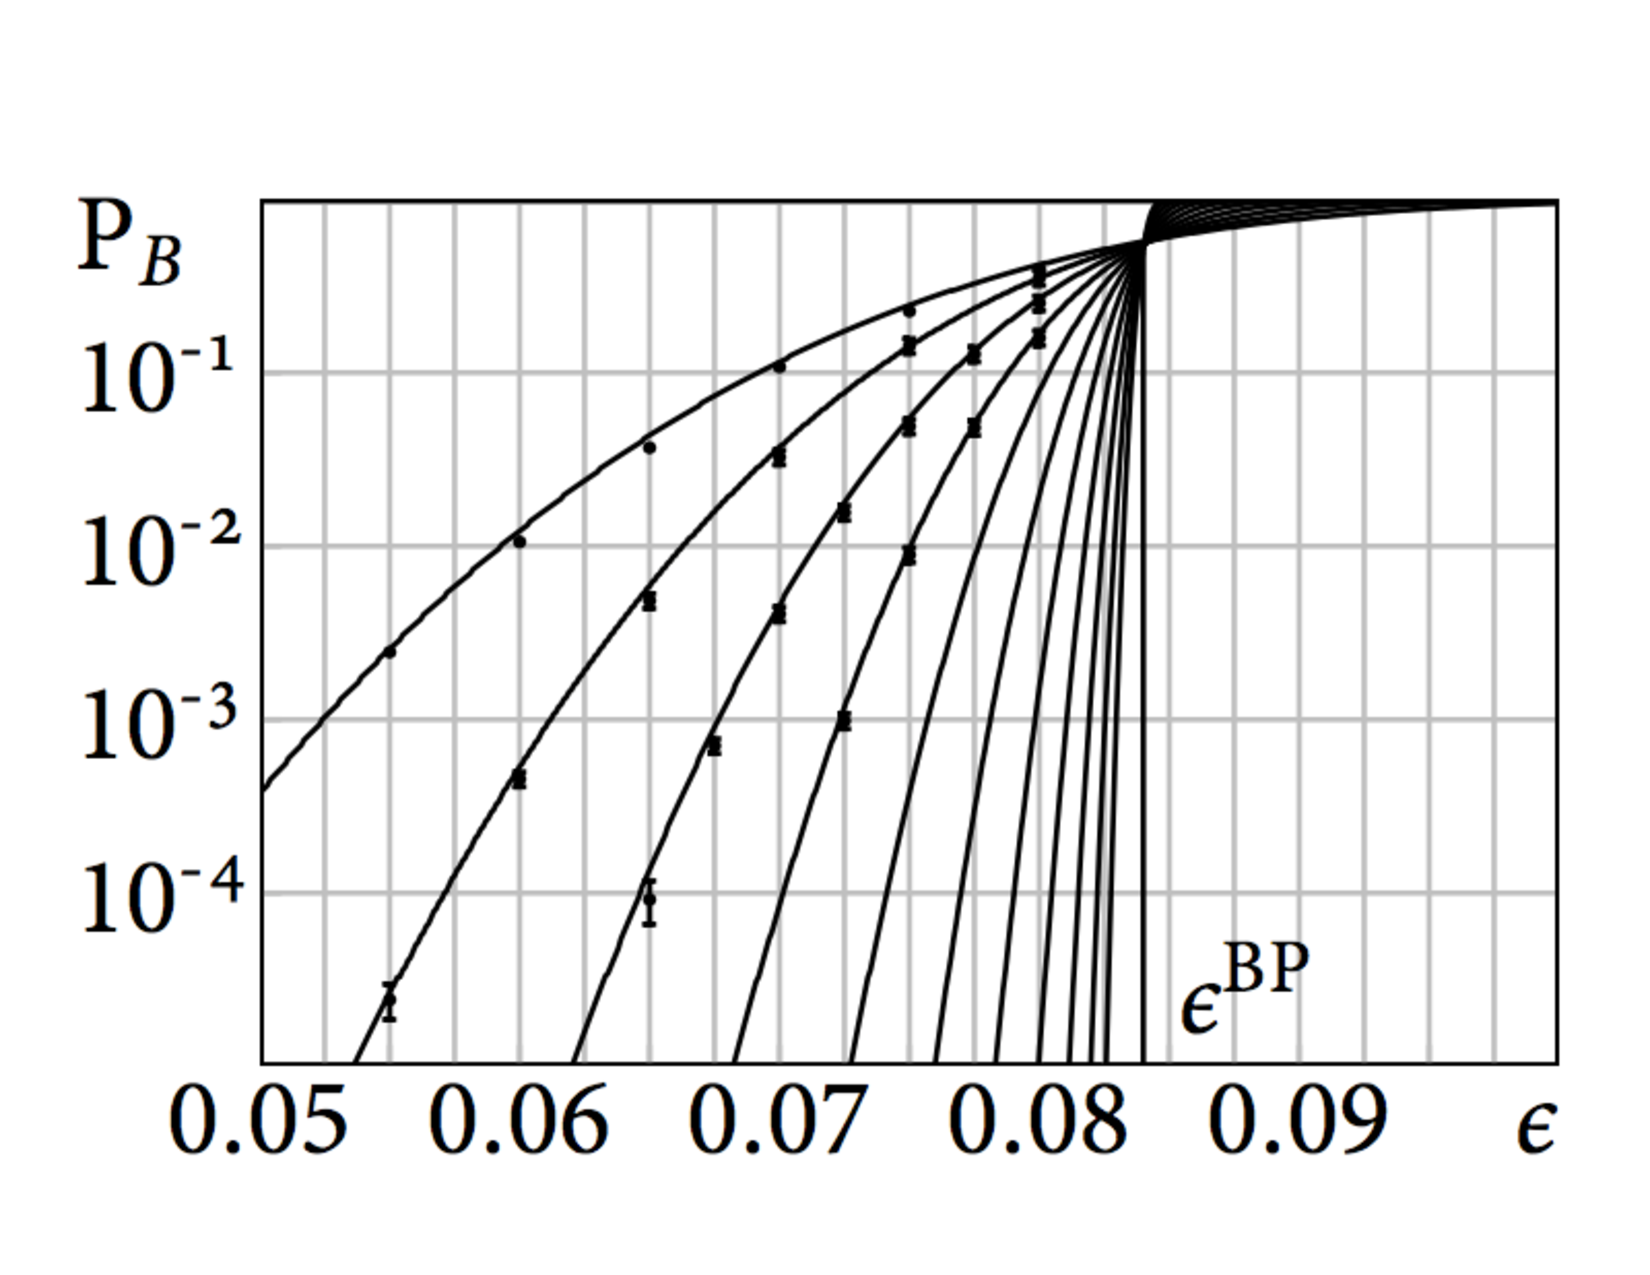
\includegraphics[width=0.6\columnwidth]{./Figures/BP_threshold_BSC.pdf}
\caption{$(3,6), P_{\text{B}}$ vs BSC($\epsilon$) for $n=2^{i}.$}
\end{figure}
\centering
$\varepsilon^{\mathrm{BP}}=0.084$, equivalent $\hbp=0.4160$\\
whereas for rate 1/2 code $\text{h}^{\mathrm{Sh}}=0.5$ 
\end{columns}
\end{frame}

\begin{frame}\frametitle{BP vs MAP}
\vspace{-5mm}
\begin{figure}
\begin{center}
\scalebox{0.5}{\begin{tikzpicture}
\def \recW{1in}; %Encoder Length
\def \recH{0.5in}; %Encoder Width

\def \R{0.06in}; %Larger circle radius

\def \Gblks{0.25in}; %Gaps between blocks
\def \ext{1.05in}; %Extensions towards left and right of the figure
\def \extB{0.25in}; %Extensions towards top of the figure

\def \fsizes{\normalsize}; %Defining a generic font size to be adjusted depending on the scaling
\def \fsize{\Large}; %Defining a generic font size to be adjusted depending on the scaling

\tikzstyle{rect}   = [ rectangle, draw, text centered, thick,
                        minimum height=\recH, minimum width=\recW ]

\node [rect](enc) at (0,0) {\fsizes{LDPC Encoder}} ;
\node[rect, right = \ext of enc] (chan){channel \LARGE{($\mathtt{h}$)} };
\node (dec)[rect,right=\ext of chan] {\fsizes Decoder} ;

\draw[<-,thick](enc)-- +(-1.6*\ext,0) node[midway,above]{\fsize $m_1,\ldots,m_k$};
\draw[->,thick](enc)--(chan)node[midway,above]{\fsize $x_1,\ldots,x_n$}node[midway,below]{\fsize $x_i\in \{0,1\}$};
\draw[->,thick](chan)--(dec)node[midway,above]{\fsize $r_1,\ldots,r_n$};

\draw[->,thick](dec)--+(1.6*\ext,0)node[midway,above]{\fsize  $\hat{m}_1,\ldots,\hat{m}_k$};

\end{tikzpicture}}
\end{center}
\end{figure}
\begin{itemize}
\item For BEC($\epsilon$), $\mathtt{h}=\epsilon$. For general BMS channel, $\text{C}^{\mathrm{Sh}}=1-\mathtt{h}$
\end{itemize}
\vspace{-5mm}
\hspace*{10pt}
\begin{columns}
\column{0.5\textwidth}
\begin{defn}{Belief Propagation (BP)}
\begin{itemize}
\item Non-optimal
\item Popular, low-complexity
\item Threshold: $\hbp$
\end{itemize}
\end{defn}
\column{0.5\textwidth}
\begin{defn}{Maximum a Posteriori (MAP)}
\begin{itemize}
\item Optimal decoder
\item \alert{Not realizable}
\item Threshold: $\hmap$
\end{itemize}
\end{defn}
\end{columns}
\centering
\onslide<2->
\begin{tabular}{|c|c|c|c|c|c|}
  \hline
  LDPC & Shannon & \multicolumn{2}{|c|}{\textcolor{blue}{AWGN}} & \multicolumn{2}{|c|}{\textcolor{blue}{BSC}} \\
  \cline{3-6}
  $(\ell,r)$ & $\texttt{h}^{\mathrm{Sh}}$ & $\hbp$ & $\hmap$ & $\hbp$ & $\hmap$ \\
  \hline
  $(3,6)$ & $0.5000$ & $0.4293$ & $0.4794$ & $0.4160$ & $0.4681$ \\
  $(4,6)$ & $0.6667$ & $0.5211$ & $0.6645$ & $0.5203$ & $0.6633$ \\
%  $(5,6)$ & $0.8333$ & $0.5731$ & $0.8333$ & $0.5773$ & $0.8333$ \\
  \hline
\end{tabular}\\
\onslide<3->
\alert{Spatial-Coupling aids in bridging this gap}
\end{frame}

%\begin{frame}{Threshold Comparison}
%\centering
%\begin{tabular}{|c|c|c|c|c|c|}
%  \hline
%  LDPC & Shannon & \multicolumn{2}{|c|}{\textcolor{blue}{AWGN}} & \multicolumn{2}{|c|}{\textcolor{blue}{BSC}} \\
%  \cline{3-6}
%  $(\ell,r)$ & $\texttt{h}^{\mathrm{Sh}}$ & $\hbp$ & $\hmap$ & $\hbp$ & $\hmap$ \\
%  \hline
%  $(3,6)$ & $0.5000$ & $0.4293$ & $0.4794$ & $0.4160$ & $0.4681$ \\
%  $(4,6)$ & $0.6667$ & $0.5211$ & $0.6645$ & $0.5203$ & $0.6633$ \\
%  $(5,6)$ & $0.8333$ & $0.5731$ & $0.8333$ & $0.5773$ & $0.8333$ \\
%  \hline
%\end{tabular}
%\\
%\onslide<2->
%\vspace{5mm}
%\alert{Spatial-Coupling aids in bridging this gap}
%\end{frame}

\begin{frame}{$(\ell,r,N,w)$ Spatially-Coupled Ensemble}
  \scalebox{0.9}{\pgfdeclarelayer{background layer}

\pgfdeclarelayer{foreground layer}

\pgfdeclarelayer{b-m layer}

\pgfsetlayers{background layer,b-m layer,main,foreground layer}


\begin{tikzpicture}[xscale=0.35,yscale=1]
  \def \offset {0.75}
  \def \eCtrl  {0.3}

  % \clip (2.5,-0.5) rectangle (25.5,5.5);

  \uncover<1> {
    \foreach \i/\text in {14/0} {
      \foreach \j in {-1,1}{
        \draw [thick] (\i+\offset*\j, 4) +(0,0) -- +(255:0.8);
        \draw [thick] (\i+\offset*\j, 4) +(0,0) -- +(270:0.8);
        \draw [thick] (\i+\offset*\j, 4) +(0,0) -- +(285:0.8);
        \draw [thick] (\i+\offset*\j, 0) +(0,0) -- +(112:0.8);
        \draw [thick] (\i+\offset*\j, 0) +(0,0) -- +(97:0.8);
        \draw [thick] (\i+\offset*\j, 0) +(0,0) -- +(82:0.8);
        \draw [thick] (\i+\offset*\j, 0) +(0,0) -- +(67:0.8);

        \node[vnodeStyle] (v\i\j) at (\i+\offset*\j, 4) {};
        \node[cnodeStyle] (c\i\j) at (\i+\offset*\j, 0) {};
      }

      \foreach \j in {0.4,3.5} {
        \node (kk) at (\i,\j) {\scriptsize{$...$}};
      }

      \node[draw,rectangle,minimum width=22pt,minimum height=16pt, fill=white] (p1_node\i) at (\i,3) {\footnotesize{$\pi\phantom{'}$}};
      \node[draw,rectangle,minimum width=22pt,minimum height=16pt, fill=white] (p2_node\i) at (\i,1) {\footnotesize{$\pi'$}};

    }

    \foreach \i/\text in {4/-N,8/-2,11/-1,14/0,17/1,20/2,24/N} {
      \node[white] at (\i,4.5) {\footnotesize{$\text$}};
    }

    \foreach \i in {6,22} {
      \node[white] (kk) at (\i,4.5) {\scriptsize{$...$}};
    }


    \foreach \i/\text in {14/0} {
      \draw[ultra thick,gray] (p2_node\i) -- (p1_node\i);
      \draw[ultra thick,gray] (p2_node\i) .. controls (\i-\eCtrl,2) .. (p1_node\i);
      \draw[ultra thick,gray] (p2_node\i) .. controls (\i+\eCtrl,2) .. (p1_node\i);
    }
  }

  \uncover<2-> {
    \foreach \i/\text in {4/-N,8/-2,11/-1,14/0,17/1,20/2,24/N} {
      \foreach \j in {-1,1}{
        \draw [thick] (\i+\offset*\j, 4) +(0,0) -- +(255:0.8);
        \draw [thick] (\i+\offset*\j, 4) +(0,0) -- +(270:0.8);
        \draw [thick] (\i+\offset*\j, 4) +(0,0) -- +(285:0.8);
        \draw [thick] (\i+\offset*\j, 0) +(0,0) -- +(112:0.8);
        \draw [thick] (\i+\offset*\j, 0) +(0,0) -- +(97:0.8);
        \draw [thick] (\i+\offset*\j, 0) +(0,0) -- +(82:0.8);
        \draw [thick] (\i+\offset*\j, 0) +(0,0) -- +(67:0.8);

        \node[vnodeStyle] (v\i\j) at (\i+\offset*\j, 4) {};
        \node[cnodeStyle] (c\i\j) at (\i+\offset*\j, 0) {};
      }

      \foreach \j in {0.4,3.5} {
        \node (kk) at (\i,\j) {\scriptsize{$...$}};
      }

      \node[draw,rectangle,minimum width=22pt,minimum height=16pt, fill=white] (p1_node\i) at (\i,3) {\footnotesize{$\pi_{\text}\phantom{'}$}};
      \node[draw,rectangle,minimum width=22pt,minimum height=16pt, fill=white] (p2_node\i) at (\i,1) {\footnotesize{$\pi_{\text}'$}};
    }

    \foreach \x in {6,22} {
      \foreach \y in {3,1} {
        \node (blu) at (\x,\y) {\footnotesize{$...$}};
      }
    }

    \foreach \i/\text in {4/-N,8/-2,11/-1,14/0,17/1,20/2,24/N} {
      \node at (\i,4.5) {\footnotesize{$\text$}};
    }

    \foreach \i in {6,22} {
      \node (kk) at (\i,4.5) {\scriptsize{$...$}};
    }
  }

  \uncover<2> {
    \foreach \i/\text in {4/-N,8/-2,11/-1,14/0,17/1,20/2,24/N} {
      \draw[ultra thick,gray] (p2_node\i) -- (p1_node\i);
      \draw[ultra thick,gray] (p2_node\i) .. controls (\i-\eCtrl,2) .. (p1_node\i);
      \draw[ultra thick,gray] (p2_node\i) .. controls (\i+\eCtrl,2) .. (p1_node\i);
    }
  }

  \uncover<3> {
    \def \midx {0.5}

    \foreach \i/\text in {-2/-\!N\!\!-\!\!2,1/-\!N\!\!-\!\!1,27/N\!+\!1,30/N\!+\!2} {
      \node at (\i,4.5) {{\color{blue} \footnotesize{$\!\text\!\!$}}};
    }

    \foreach \i/\text in {-2/-\!N\!-\!2,1/-\!N\!-\!1} {
      \foreach \j in {-1,1}{
        \draw [thick, color=blue!70] (\i+\offset*\j, 4) +(0,0) -- +(255:0.8);
        \draw [thick, color=blue!70] (\i+\offset*\j, 4) +(0,0) -- +(270:0.8);
        \draw [thick, color=blue!70] (\i+\offset*\j, 4) +(0,0) -- +(285:0.8);

        \node[vnodeStyle, fill=blue!20, draw=blue!70] (v\i\j) at (\i+\offset*\j, 4) {};
      }

      \node[draw,rectangle,minimum width=22pt,minimum height=16pt, fill=blue!20, draw=blue!70] (p1_node\i) at (\i,3) {\footnotesize{$\!\pi_{\text}\phantom{'}\!\!$}};

      \foreach \j in {3.5} {
        \node (kk) at (\i,\j) {\scriptsize{$...$}};
      }
    }

    \foreach \i/\j in {-2/4, 1/4} {
      \draw[color=blue!50] (p1_node\i) -- (p2_node\j);
      \draw[color=blue!50] (p1_node\i) .. controls (\i*\midx+\j*\midx-0.2,2) .. (p2_node\j);
      \draw[color=blue!50] (p1_node\i) .. controls (\i*\midx+\j*\midx+0.2,2) .. (p2_node\j);
    }
    \foreach \i in {1} {
      \draw[color=blue!50] (p1_node\i) -- (9*0.35, 2.2);
      \draw[color=blue!50] (p1_node\i) -- (9*0.35-0.2, 2.2);
      \draw[color=blue!50] (p1_node\i) -- (9*0.35+0.2, 2.2);
    }


    \foreach \i/\text in {27/N+1,30/N+2} {
      \foreach \j in {-1,1}{
        \draw [thick, color=blue!70] (\i+\offset*\j, 4) +(0,0) -- +(255:0.8);
        \draw [thick, color=blue!70] (\i+\offset*\j, 4) +(0,0) -- +(270:0.8);
        \draw [thick, color=blue!70] (\i+\offset*\j, 4) +(0,0) -- +(285:0.8);

        \node[vnodeStyle, fill=blue!20, draw=blue!70] (v\i\j) at (\i+\offset*\j, 4) {};
      }

      \node[draw,rectangle,minimum width=22pt,minimum height=16pt, fill=blue!20, draw=blue!70] (p1_node\i) at (\i,3) {\footnotesize{$\!\pi_{\text}\phantom{'}\!\!$}};

      \foreach \j in {3.5} {
        \node (kk) at (\i,\j) {\scriptsize{$...$}};
      }
    }

  }

  \uncover<3> {

    \foreach \i/\text in {27/N+1,30/N+2} {
      \foreach \j in {-1,1}{
        \draw [thick] (\i+\offset*\j, 0) +(0,0) -- +(112:0.8);
        \draw [thick] (\i+\offset*\j, 0) +(0,0) -- +(97:0.8);
        \draw [thick] (\i+\offset*\j, 0) +(0,0) -- +(82:0.8);
        \draw [thick] (\i+\offset*\j, 0) +(0,0) -- +(67:0.8);

        \node[cnodeStyle] (c\i\j) at (\i+\offset*\j, 0) {};
      }
      \node[draw,rectangle,minimum width=22pt,minimum height=16pt, fill=white] (p2_node\i) at (\i,1) {\footnotesize{$\!\pi_{\text}'\!\!$}};

      \foreach \j in {0.4} {
        \node (kk) at (\i,\j) {\scriptsize{$...$}};
      }
    }
  }

  \uncover<3> {
    \foreach \i/\j in {27/27, 27/30, 30/30} {
      \draw[color=blue!50] (p1_node\i) -- (p2_node\j);
      \draw[color=blue!50] (p1_node\i) .. controls (\i*\midx+\j*\midx-0.2,2) .. (p2_node\j);
      \draw[color=blue!50] (p1_node\i) .. controls (\i*\midx+\j*\midx+0.2,2) .. (p2_node\j);
    }
  }


  \uncover<3> {
    \draw[gray] (p1_node4) -- (p2_node4);
    \draw[gray] (p1_node4) .. controls (8*\midx-0.2,2) .. (p2_node4);
    \draw[gray] (p1_node4) .. controls (8*\midx+0.2,2) .. (p2_node4);
    \foreach \i/\j in {4/8,4/11} {
      \draw[gray] (p1_node\i) -- node[fill=white, minimum size=10pt]  {} (p2_node\j);
      \draw[gray] (p1_node\i) .. controls (\i*\midx+\j*\midx-0.2,2) .. node[fill=white, minimum size=10pt]{} (p2_node\j);
      \draw[gray] (p1_node\i) .. controls (\i*\midx+\j*\midx+0.2,2) .. node[fill=white, minimum size=10pt]{} (p2_node\j);
    }

    \draw (8,1) +(131:1.2) node (tt0) {};
    \draw (8,1) +(136:1.3) node (tt1) {};
    \draw (8,1) +(141:1.4) node (tt2) {};
    \draw[gray] (p2_node8) -- (tt0);
    \draw[gray] (p2_node8) -- (tt1);
    \draw[gray] (p2_node8) -- (tt2);
    \foreach \i/\j in {8/8,8/11,8/14} {
      \draw[gray] (p1_node\i) -- (p2_node\j);
      \draw[gray] (p1_node\i) .. controls (\i*\midx+\j*\midx-0.2,2) .. (p2_node\j);
      \draw[gray] (p1_node\i) .. controls (\i*\midx+\j*\midx+0.2,2) .. (p2_node\j);
    }

    \foreach \i/\j in {11/11,11/14,11/17} {
      \draw[gray] (p1_node\i) -- (p2_node\j);
      \draw[gray] (p1_node\i) .. controls (\i*\midx+\j*\midx-0.2,2) .. (p2_node\j);
      \draw[gray] (p1_node\i) .. controls (\i*\midx+\j*\midx+0.2,2) .. (p2_node\j);
    }

    \foreach \i/\j in {14/14,14/17,14/20} {
      \draw[gray] (p1_node\i) -- (p2_node\j);
      \draw[gray] (p1_node\i) .. controls (\i*\midx+\j*\midx-0.2,2) .. (p2_node\j);
      \draw[gray] (p1_node\i) .. controls (\i*\midx+\j*\midx+0.2,2) .. (p2_node\j);
    }

    \foreach \i/\j in {17/17,17/20} {
      \draw[gray] (p1_node\i) -- (p2_node\j);
      \draw[gray] (p1_node\i) .. controls (\i*\midx+\j*\midx-0.2,2) .. (p2_node\j);
      \draw[gray] (p1_node\i) .. controls (\i*\midx+\j*\midx+0.2,2) .. (p2_node\j);
    }
    \draw[gray] (p1_node17) -- node[fill=white, minimum size=10pt] {}
    (p2_node24);
    \draw[gray] (p1_node17) .. controls (41*\midx-0.2,2) .. node[fill=white, minimum size=10pt]{} (p2_node24);
    \draw[gray] (p1_node17) .. controls (41*\midx+0.2,2) .. node[fill=white, minimum size=10pt]{} (p2_node24);
    \draw[gray] (p1_node20) -- (p2_node20);
    \draw[gray] (p1_node20) .. controls (40*\midx-0.2,2) .. (p2_node20);
    \draw[gray] (p1_node20) .. controls (40*\midx+0.2,2) .. (p2_node20);
    \foreach \i/\j in {20/24,20/27} {
      \draw[gray] (p1_node\i) -- node[fill=white, minimum size=10pt] {}
      (p2_node\j);
      \draw[gray] (p1_node\i) .. controls (\i*\midx+\j*\midx-0.2,2) .. node[fill=white, minimum size=10pt]{} (p2_node\j);
      \draw[gray] (p1_node\i) .. controls (\i*\midx+\j*\midx+0.2,2) .. node[fill=white, minimum size=10pt]{} (p2_node\j);
    }

    \foreach \i/\j in {24/24,24/27,24/30} {
      \draw[gray] (p1_node\i) -- (p2_node\j);
      \draw[gray] (p1_node\i) .. controls (\i*\midx+\j*\midx-0.2,2) .. (p2_node\j);
      \draw[gray] (p1_node\i) .. controls (\i*\midx+\j*\midx+0.2,2) .. (p2_node\j);
    }

  }
\end{tikzpicture}


%%% Local Variables: 
%%% mode: latex
%%% TeX-master: "../ita2016"
%%% End: 
}
  \begin{itemize}
  \item<1> An LDPC code of left-degree $\ell=3$ and right-degree $r=4$
  \item<3-> Shown for $\ell = 3$, $r = 4$, and $w=3$
  \item<3-> Check-nodes at Section $\{i\}$ are connected to variable-nodes in Sections $\{i-(w-1),\dots,i\}$
  \item<3-> Shown to have {\blue near optimal BP thresholds}
  \end{itemize}
\end{frame}

\subsection{Threshold Saturation Phenomenon}
\begin{frame}{Threshold Saturation via Spatial Coupling (1)}
\begin{center}
\scalebox{0.5}{
\begin{tikzpicture}
  [node distance=1cm,draw=black,thick, >=stealth']
  \draw[<->,line width=2pt] (-7,0) -- (9,0) ;
  \node[circle,draw=red,minimum size=4mm,fill=red] (hbp) at (-1,0) {};
  \node[circle,draw=red,minimum size=4mm,fill=red] (hmap) at (5,0) {};
  \node[circle,draw=green!30!black!70,minimum size=4mm,fill=green!30!black!70] (h) at (-5,0) {};
  \node at (-1,1.3) {\huge{$\h^{\mathrm{BP}}$}}
     edge[->] (hbp);
  \node at (5,1.3) {\huge{$\h^{\mathrm{MAP}}$}}
     edge[->] (hmap);
  \node at (-5,1.3) {\huge{$\h$}}
     edge[->] (h);
\end{tikzpicture}
}
\end{center}
\begin{columns}
  \column{0.45\textwidth}
  \begin{center}
    \setlength\tikzheight{3cm} 
    \setlength\tikzwidth{3.5cm} 
    % This file was created by matlab2tikz v0.1.2.
% Copyright (c) 2008--2011, Nico Schlömer <nico.schloemer@gmail.com>
% All rights reserved.
% 
% The latest updates can be retrieved from
%   http://www.mathworks.com/matlabcentral/fileexchange/22022-matlab2tikz
% where you can also make suggestions and rate matlab2tikz.
% 
\begin{tikzpicture}

\begin{axis}[%
scale only axis,
width=\tikzwidth,
height=\tikzheight,
xmin=0, xmax=20,
ymin=0, ymax=0.35,
xlabel={Check-node Group Index},
ylabel={Message Error},
title={Uncoupled},
axis on top]

\only<1>{
\addplot [thick,ycomb,color=blue,solid,mark=o,mark options={solid}]
coordinates{
 (1,0.35)(2,0.35)(3,0.35)(4,0.35)(5,0.35)(6,0.35)(7,0.35)(8,0.35)(9,0.35)(10,0.35)(11,0.35)(12,0.35)(13,0.35)(14,0.35)(15,0.35)(16,0.35)(17,0.35)(18,0.35)(19,0.35) 
};
}

\only<2>{
\addplot [thick,ycomb,color=blue,solid,mark=o,mark options={solid}]
coordinates{
 (1,0.273492)(2,0.273492)(3,0.273492)(4,0.273492)(5,0.273492)(6,0.273492)(7,0.273492)(8,0.273492)(9,0.273492)(10,0.273492)(11,0.273492)(12,0.273492)(13,0.273492)(14,0.273492)(15,0.273492)(16,0.273492)(17,0.273492)(18,0.273492)(19,0.273492) 
};
}

\only<3>{
\addplot [thick,ycomb,color=blue,solid,mark=o,mark options={solid}]
coordinates{
 (1,0.22266)(2,0.22266)(3,0.22266)(4,0.22266)(5,0.22266)(6,0.22266)(7,0.22266)(8,0.22266)(9,0.22266)(10,0.22266)(11,0.22266)(12,0.22266)(13,0.22266)(14,0.22266)(15,0.22266)(16,0.22266)(17,0.22266)(18,0.22266)(19,0.22266) 
};
}

\only<4>{
\addplot [thick,ycomb,color=blue,solid,mark=o,mark options={solid}]
coordinates{
 (1,0.179516)(2,0.179516)(3,0.179516)(4,0.179516)(5,0.179516)(6,0.179516)(7,0.179516)(8,0.179516)(9,0.179516)(10,0.179516)(11,0.179516)(12,0.179516)(13,0.179516)(14,0.179516)(15,0.179516)(16,0.179516)(17,0.179516)(18,0.179516)(19,0.179516) 
};
}

\only<5>{
\addplot [thick,ycomb,color=blue,solid,mark=o,mark options={solid}]
coordinates{
 (1,0.138107)(2,0.138107)(3,0.138107)(4,0.138107)(5,0.138107)(6,0.138107)(7,0.138107)(8,0.138107)(9,0.138107)(10,0.138107)(11,0.138107)(12,0.138107)(13,0.138107)(14,0.138107)(15,0.138107)(16,0.138107)(17,0.138107)(18,0.138107)(19,0.138107) 
};
}

\only<6>{
\addplot [thick,ycomb,color=blue,solid,mark=o,mark options={solid}]
coordinates{
 (1,0.096238)(2,0.096238)(3,0.096238)(4,0.096238)(5,0.096238)(6,0.096238)(7,0.096238)(8,0.096238)(9,0.096238)(10,0.096238)(11,0.096238)(12,0.096238)(13,0.096238)(14,0.096238)(15,0.096238)(16,0.096238)(17,0.096238)(18,0.096238)(19,0.096238) 
};
}

\only<7>{
\addplot [thick,ycomb,color=blue,solid,mark=o,mark options={solid}]
coordinates{
 (1,0.0551812)(2,0.0551812)(3,0.0551812)(4,0.0551812)(5,0.0551812)(6,0.0551812)(7,0.0551812)(8,0.0551812)(9,0.0551812)(10,0.0551812)(11,0.0551812)(12,0.0551812)(13,0.0551812)(14,0.0551812)(15,0.0551812)(16,0.0551812)(17,0.0551812)(18,0.0551812)(19,0.0551812) 
};
}

\only<8>{
\addplot [thick,ycomb,color=blue,solid,mark=o,mark options={solid}]
coordinates{
 (1,0.0213689)(2,0.0213689)(3,0.0213689)(4,0.0213689)(5,0.0213689)(6,0.0213689)(7,0.0213689)(8,0.0213689)(9,0.0213689)(10,0.0213689)(11,0.0213689)(12,0.0213689)(13,0.0213689)(14,0.0213689)(15,0.0213689)(16,0.0213689)(17,0.0213689)(18,0.0213689)(19,0.0213689) 
};
}

\only<9>{
\addplot [thick,ycomb,color=blue,solid,mark=o,mark options={solid}]
coordinates{
 (1,0.0036682)(2,0.0036682)(3,0.0036682)(4,0.0036682)(5,0.0036682)(6,0.0036682)(7,0.0036682)(8,0.0036682)(9,0.0036682)(10,0.0036682)(11,0.0036682)(12,0.0036682)(13,0.0036682)(14,0.0036682)(15,0.0036682)(16,0.0036682)(17,0.0036682)(18,0.0036682)(19,0.0036682) 
};
}

\end{axis}
\end{tikzpicture}

  \end{center}
  \column{0.45\textwidth}
  \begin{center}
    \setlength\tikzheight{3cm} 
    \setlength\tikzwidth{3.5cm} 
    % This file was created by matlab2tikz v0.1.2.
% Copyright (c) 2008--2011, Nico Schlömer <nico.schloemer@gmail.com>
% All rights reserved.
% 
% The latest updates can be retrieved from
%   http://www.mathworks.com/matlabcentral/fileexchange/22022-matlab2tikz
% where you can also make suggestions and rate matlab2tikz.
% 
\begin{tikzpicture}

% defining custom colors

\begin{axis}[%
scale only axis,
width=\tikzwidth,
height=\tikzheight,
xmin=0, xmax=20,
ymin=0, ymax=0.35,
xlabel={Check-node Group Index},
title={Spatially Coupled},
ylabel={Message Error},
axis on top]

\only<1>{
\addplot [thick,ycomb,color=blue,solid,mark=o,mark options={solid}]
coordinates{
 (1,0.116667)(2,0.233333)(3,0.35)(4,0.35)(5,0.35)(6,0.35)(7,0.35)(8,0.35)(9,0.35)(10,0.35)(11,0.35)(12,0.35)(13,0.35)(14,0.35)(15,0.35)(16,0.35)(17,0.35)(18,0.233333)(19,0.116667) 
};
}

\only<2>{
\addplot [thick,ycomb,color=blue,solid,mark=o,mark options={solid}]
coordinates{
 (1,0.056153)(2,0.137371)(3,0.228535)(4,0.263545)(5,0.273492)(6,0.273492)(7,0.273492)(8,0.273492)(9,0.273492)(10,0.273492)(11,0.273492)(12,0.273492)(13,0.273492)(14,0.273492)(15,0.273492)(16,0.263545)(17,0.228535)(18,0.137371)(19,0.056153) 
};
}

\only<3>{
\addplot [thick,ycomb,color=blue,solid,mark=o,mark options={solid}]
coordinates{
 (1,0.0291678)(2,0.0827153)(3,0.151749)(4,0.195921)(5,0.216593)(6,0.221779)(7,0.22266)(8,0.22266)(9,0.22266)(10,0.22266)(11,0.22266)(12,0.22266)(13,0.22266)(14,0.221779)(15,0.216593)(16,0.195921)(17,0.151749)(18,0.0827153)(19,0.0291678) 
};
}

\only<4>{
\addplot [thick,ycomb,color=blue,solid,mark=o,mark options={solid}]
coordinates{
 (1,0.0142646)(2,0.0464335)(3,0.0947015)(4,0.136701)(5,0.163657)(6,0.175138)(7,0.178712)(8,0.179426)(9,0.179516)(10,0.179516)(11,0.179516)(12,0.179426)(13,0.178712)(14,0.175138)(15,0.163657)(16,0.136701)(17,0.0947015)(18,0.0464335)(19,0.0142646) 
};
}

\only<5>{
\addplot [thick,ycomb,color=blue,solid,mark=o,mark options={solid}]
coordinates{
 (1,0.00586824)(2,0.022245)(3,0.0515369)(4,0.08444)(5,0.111726)(6,0.127883)(7,0.135048)(8,0.137411)(9,0.137998)(10,0.138087)(11,0.137998)(12,0.137411)(13,0.135048)(14,0.127883)(15,0.111726)(16,0.08444)(17,0.0515369)(18,0.022245)(19,0.00586824) 
};
}

\only<6>{
\addplot [thick,ycomb,color=blue,solid,mark=o,mark options={solid}]
coordinates{
 (1,0.00175399)(2,0.00802468)(3,0.0219409)(4,0.0420654)(5,0.063364)(6,0.0799438)(7,0.0897087)(8,0.0941259)(9,0.0956824)(10,0.0960254)(11,0.0956824)(12,0.0941259)(13,0.0897087)(14,0.0799438)(15,0.063364)(16,0.0420654)(17,0.0219409)(18,0.00802468)(19,0.00175399) 
};
}

\only<7>{
\addplot [thick,ycomb,color=blue,solid,mark=o,mark options={solid}]
coordinates{
 (1,0.000304318)(2,0.00178386)(3,0.00610694)(4,0.0143752)(5,0.0257247)(6,0.037249)(7,0.0461243)(8,0.0513925)(9,0.0538026)(10,0.0544518)(11,0.0538026)(12,0.0513925)(13,0.0461243)(14,0.037249)(15,0.0257247)(16,0.0143752)(17,0.00610694)(18,0.00178386)(19,0.000304318) 
};
}

\only<8>{
\addplot [thick,ycomb,color=blue,solid,mark=o,mark options={solid}]
coordinates{
 (1,2.13384e-05)(2,0.000175043)(3,0.000814929)(4,0.00251955)(5,0.0056764)(6,0.00994033)(7,0.0142749)(8,0.0176403)(9,0.0195943)(10,0.0202096)(11,0.0195943)(12,0.0176403)(13,0.0142749)(14,0.00994033)(15,0.0056764)(16,0.00251955)(17,0.000814929)(18,0.000175043)(19,2.13384e-05) 
};
}

\only<9>{
\addplot [thick,ycomb,color=blue,solid,mark=o,mark options={solid}]
coordinates{
 (1,3.30536e-07)(2,4.29016e-06)(3,3.01497e-05)(4,0.000133237)(5,0.000406167)(6,0.000915727)(7,0.0016142)(8,0.00232761)(9,0.0028485)(10,0.00303691)(11,0.0028485)(12,0.00232761)(13,0.0016142)(14,0.000915727)(15,0.000406167)(16,0.000133237)(17,3.01497e-05)(18,4.29016e-06)(19,3.30536e-07) 
};
}

\end{axis}
\end{tikzpicture}

  \end{center}
\end{columns}
\end{frame}

\begin{frame}
\frametitle{Threshold Saturation via Spatial Coupling (2)}
\begin{center}
\scalebox{0.5}{
\begin{tikzpicture}
  [node distance=1cm,draw=black,thick, >=stealth']
  \draw[<->,line width=2pt] (-7,0) -- (9,0) ;
  \node[circle,draw=red,minimum size=4mm,fill=red] (hbp) at (-1,0) {};
  \node[circle,draw=red,minimum size=4mm,fill=red] (hmap) at (5,0) {};
  \node[circle,draw=green!30!black!70,minimum size=4mm,fill=green!30!black!70] (h) at (3,0) {};
  \node at (-1,1.3) {\huge{$\h^{\mathrm{BP}}$}}
     edge[->] (hbp);
  \node at (5,1.3) {\huge{$\h^{\mathrm{MAP}}$}}
     edge[->] (hmap);
  \node at (3,1.3) {\huge{$\h$}}
     edge[->] (h);
\end{tikzpicture}
}
\end{center}
\begin{columns}
  \column{0.45\textwidth}
  \begin{center}
    \setlength\tikzheight{3cm} 
    \setlength\tikzwidth{3.5cm} 
    % This file was created by matlab2tikz v0.1.2.
% Copyright (c) 2008--2011, Nico Schlömer <nico.schloemer@gmail.com>
% All rights reserved.
% 
% The latest updates can be retrieved from
%   http://www.mathworks.com/matlabcentral/fileexchange/22022-matlab2tikz
% where you can also make suggestions and rate matlab2tikz.
% 
\begin{tikzpicture}

\begin{axis}[
scale only axis,
width=\tikzwidth,
height=\tikzheight,
xmin=0, xmax=20,
ymin=0, ymax=0.5,
xlabel={Check-node Group Index},
ylabel={Message Error},
title={Uncoupled},
axis on top]

\only<1>{
\addplot [thick,ycomb,color=blue,solid,mark=o,mark options={solid}]
coordinates{
 (1,0.45)(2,0.45)(3,0.45)(4,0.45)(5,0.45)(6,0.45)(7,0.45)(8,0.45)(9,0.45)(10,0.45)(11,0.45)(12,0.45)(13,0.45)(14,0.45)(15,0.45)(16,0.45)(17,0.45)(18,0.45)(19,0.45) 
};
}

\only<2>{
\addplot [thick,ycomb,color=blue,solid,mark=o,mark options={solid}]
coordinates{
 (1,0.385826)(2,0.385826)(3,0.385826)(4,0.385826)(5,0.385826)(6,0.385826)(7,0.385826)(8,0.385826)(9,0.385826)(10,0.385826)(11,0.385826)(12,0.385826)(13,0.385826)(14,0.385826)(15,0.385826)(16,0.385826)(17,0.385826)(18,0.385826)(19,0.385826) 
};
}

\only<3>{
\addplot [thick,ycomb,color=blue,solid,mark=o,mark options={solid}]
coordinates{
 (1,0.368129)(2,0.368129)(3,0.368129)(4,0.368129)(5,0.368129)(6,0.368129)(7,0.368129)(8,0.368129)(9,0.368129)(10,0.368129)(11,0.368129)(12,0.368129)(13,0.368129)(14,0.368129)(15,0.368129)(16,0.368129)(17,0.368129)(18,0.368129)(19,0.368129) 
};
}

\only<4>{
\addplot [thick,ycomb,color=blue,solid,mark=o,mark options={solid}]
coordinates{
 (1,0.361161)(2,0.361161)(3,0.361161)(4,0.361161)(5,0.361161)(6,0.361161)(7,0.361161)(8,0.361161)(9,0.361161)(10,0.361161)(11,0.361161)(12,0.361161)(13,0.361161)(14,0.361161)(15,0.361161)(16,0.361161)(17,0.361161)(18,0.361161)(19,0.361161) 
};
}

\only<5>{
\addplot [thick,ycomb,color=blue,solid,mark=o,mark options={solid}]
coordinates{
 (1,0.3581)(2,0.3581)(3,0.3581)(4,0.3581)(5,0.3581)(6,0.3581)(7,0.3581)(8,0.3581)(9,0.3581)(10,0.3581)(11,0.3581)(12,0.3581)(13,0.3581)(14,0.3581)(15,0.3581)(16,0.3581)(17,0.3581)(18,0.3581)(19,0.3581) 
};
}

\only<6>{
\addplot [thick,ycomb,color=blue,solid,mark=o,mark options={solid}]
coordinates{
 (1,0.356694)(2,0.356694)(3,0.356694)(4,0.356694)(5,0.356694)(6,0.356694)(7,0.356694)(8,0.356694)(9,0.356694)(10,0.356694)(11,0.356694)(12,0.356694)(13,0.356694)(14,0.356694)(15,0.356694)(16,0.356694)(17,0.356694)(18,0.356694)(19,0.356694) 
};
}

\only<7>{
\addplot [thick,ycomb,color=blue,solid,mark=o,mark options={solid}]
coordinates{
 (1,0.356036)(2,0.356036)(3,0.356036)(4,0.356036)(5,0.356036)(6,0.356036)(7,0.356036)(8,0.356036)(9,0.356036)(10,0.356036)(11,0.356036)(12,0.356036)(13,0.356036)(14,0.356036)(15,0.356036)(16,0.356036)(17,0.356036)(18,0.356036)(19,0.356036) 
};
}

\only<8->{
\addplot [thick,ycomb,color=blue,solid,mark=o,mark options={solid}]
coordinates{
 (1,0.355725)(2,0.355725)(3,0.355725)(4,0.355725)(5,0.355725)(6,0.355725)(7,0.355725)(8,0.355725)(9,0.355725)(10,0.355725)(11,0.355725)(12,0.355725)(13,0.355725)(14,0.355725)(15,0.355725)(16,0.355725)(17,0.355725)(18,0.355725)(19,0.355725) 
};
}

\end{axis}
\end{tikzpicture}

  \end{center}
  \column{0.45\textwidth}
  \begin{center}
    \setlength\tikzheight{3cm}
    \setlength\tikzwidth{3.5cm}
    % This file was created by matlab2tikz v0.1.2.
% Copyright (c) 2008--2011, Nico Schlömer <nico.schloemer@gmail.com>
% All rights reserved.
% 
% The latest updates can be retrieved from
%   http://www.mathworks.com/matlabcentral/fileexchange/22022-matlab2tikz
% where you can also make suggestions and rate matlab2tikz.
% 
\begin{tikzpicture}

\begin{axis}[
scale only axis,
width=\tikzwidth,
height=\tikzheight,
xmin=0, xmax=20,
ymin=0, ymax=0.5,
xlabel={Check-node Group Index},
ylabel={Message Error},
title={Spatially Coupled},
axis on top]

\only<1>{
\addplot [thick,ycomb,color=blue,solid,mark=o,mark options={solid}]
coordinates{
 (1,0.15)(2,0.3)(3,0.45)(4,0.45)(5,0.45)(6,0.45)(7,0.45)(8,0.45)(9,0.45)(10,0.45)(11,0.45)(12,0.45)(13,0.45)(14,0.45)(15,0.45)(16,0.45)(17,0.45)(18,0.3)(19,0.15) 
};
}

\only<2>{
\addplot [thick,ycomb,color=blue,solid,mark=o,mark options={solid}]
coordinates{
 (1,0.0644873)(2,0.169171)(3,0.293334)(4,0.356801)(5,0.380726)(6,0.385171)(7,0.385826)(8,0.385826)(9,0.385826)(10,0.385826)(11,0.385826)(12,0.385826)(13,0.385826)(14,0.385171)(15,0.380726)(16,0.356801)(17,0.293334)(18,0.169171)(19,0.0644873) 
};
}

\only<3>{
\addplot [thick,ycomb,color=blue,solid,mark=o,mark options={solid}]
coordinates{
 (1,0.0381925)(2,0.115522)(3,0.221613)(4,0.30116)(5,0.345369)(6,0.361756)(7,0.366695)(8,0.367863)(9,0.368094)(10,0.368123)(11,0.368094)(12,0.367863)(13,0.366695)(14,0.361756)(15,0.345369)(16,0.30116)(17,0.221613)(18,0.115522)(19,0.0381925) 
};
}

\only<4>{
\addplot [thick,ycomb,color=blue,solid,mark=o,mark options={solid}]
coordinates{
 (1,0.0242946)(2,0.0825159)(3,0.173261)(4,0.25791)(5,0.316331)(6,0.344869)(7,0.356023)(8,0.359699)(9,0.360777)(10,0.360997)(11,0.360777)(12,0.359699)(13,0.356023)(14,0.344869)(15,0.316331)(16,0.25791)(17,0.173261)(18,0.0825159)(19,0.0242946) 
};
}

\only<5>{
\addplot [thick,ycomb,color=blue,solid,mark=o,mark options={solid}]
coordinates{
 (1,0.0154232)(2,0.0587633)(3,0.13537)(4,0.220047)(5,0.288691)(6,0.328879)(7,0.34731)(8,0.354424)(9,0.356856)(10,0.357422)(11,0.356856)(12,0.354424)(13,0.34731)(14,0.328879)(15,0.288691)(16,0.220047)(17,0.13537)(18,0.0587633)(19,0.0154232) 
};
}

\only<6>{
\addplot [thick,ycomb,color=blue,solid,mark=o,mark options={solid}]
coordinates{
 (1,0.00938825)(2,0.0405862)(3,0.103635)(4,0.184829)(5,0.260484)(6,0.311715)(7,0.338358)(8,0.349778)(9,0.354025)(10,0.355074)(11,0.354025)(12,0.349778)(13,0.338358)(14,0.311715)(15,0.260484)(16,0.184829)(17,0.103635)(18,0.0405862)(19,0.00938825) 
};
}

\only<7>{
\addplot [thick,ycomb,color=blue,solid,mark=o,mark options={solid}]
coordinates{
 (1,0.00531349)(2,0.0266129)(3,0.0765848)(4,0.151337)(5,0.230827)(6,0.292194)(7,0.327964)(8,0.3447)(9,0.351308)(10,0.352997)(11,0.351308)(12,0.3447)(13,0.327964)(14,0.292194)(15,0.230827)(16,0.151337)(17,0.0765848)(18,0.0266129)(19,0.00531349) 
};
}

\only<8>{
\addplot [thick,ycomb,color=blue,solid,mark=o,mark options={solid}]
coordinates{
 (1,0.0027223)(2,0.0162662)(3,0.0539349)(4,0.119714)(5,0.199592)(6,0.269563)(7,0.315197)(8,0.338455)(9,0.348145)(10,0.350688)(11,0.348145)(12,0.338455)(13,0.315197)(14,0.269563)(15,0.199592)(16,0.119714)(17,0.0539349)(18,0.0162662)(19,0.0027223) 
};
}

\only<9>{
\addplot [thick,ycomb,color=blue,solid,mark=o,mark options={solid}]
coordinates{
 (1,0.00123406)(2,0.00912365)(3,0.0357976)(4,0.0907383)(5,0.167346)(6,0.243516)(7,0.299242)(8,0.330341)(9,0.344056)(10,0.347751)(11,0.344056)(12,0.330341)(13,0.299242)(14,0.243516)(15,0.167346)(16,0.0907383)(17,0.0357976)(18,0.00912365)(19,0.00123406) 
};
}

\only<10>{
\addplot [thick,ycomb,color=blue,solid,mark=o,mark options={solid}]
coordinates{
 (1,0.000486018)(2,0.00463517)(3,0.0221733)(4,0.0654017)(5,0.135229)(6,0.214305)(7,0.279461)(8,0.319602)(9,0.338502)(10,0.343751)(11,0.338502)(12,0.319602)(13,0.279461)(14,0.214305)(15,0.135229)(16,0.0654017)(17,0.0221733)(18,0.00463517)(19,0.000486018) 
};
}

\only<11>{
\addplot [thick,ycomb,color=blue,solid,mark=o,mark options={solid}]
coordinates{
 (1,0.000163825)(2,0.00210784)(3,0.0126959)(4,0.0444965)(5,0.104693)(6,0.182779)(7,0.255545)(8,0.305446)(9,0.330806)(10,0.338117)(11,0.330806)(12,0.305446)(13,0.255545)(14,0.182779)(15,0.104693)(16,0.0444965)(17,0.0126959)(18,0.00210784)(19,0.000163825) 
};
}

\only<12>{
\addplot [thick,ycomb,color=blue,solid,mark=o,mark options={solid}]
coordinates{
 (1,4.65515e-05)(2,0.000847044)(3,0.00664797)(4,0.0283438)(5,0.0771533)(6,0.150255)(7,0.22764)(8,0.287113)(9,0.320099)(10,0.330055)(11,0.320099)(12,0.287113)(13,0.22764)(14,0.150255)(15,0.0771533)(16,0.0283438)(17,0.00664797)(18,0.000847044)(19,4.65515e-05) 
};
}

\only<13>{
\addplot [thick,ycomb,color=blue,solid,mark=o,mark options={solid}]
coordinates{
 (1,1.09359e-05)(2,0.000295967)(3,0.00314042)(4,0.0167312)(5,0.0536961)(6,0.118281)(7,0.196367)(8,0.263972)(9,0.305275)(10,0.318442)(11,0.305275)(12,0.263972)(13,0.196367)(14,0.118281)(15,0.0536961)(16,0.0167312)(17,0.00314042)(18,0.000295967)(19,1.09359e-05) 
};
}

\only<14>{
\addplot [thick,ycomb,color=blue,solid,mark=o,mark options={solid}]
coordinates{
 (1,2.06538e-06)(2,8.7932e-05)(3,0.00131355)(4,0.00902068)(5,0.0349007)(6,0.088359)(7,0.162722)(8,0.235566)(9,0.284916)(10,0.301654)(11,0.284916)(12,0.235566)(13,0.162722)(14,0.088359)(15,0.0349007)(16,0.00902068)(17,0.00131355)(18,8.7932e-05)(19,2.06538e-06) 
};
}

\only<15>{
\addplot [thick,ycomb,color=blue,solid,mark=o,mark options={solid}]
coordinates{
 (1,0)(2,0)(3,0)(4,0)(5,0)(6,0)(7,0)(8,0)(9,0)(10,0)(11,0)(12,0)(13,0)(14,0)(15,0)(16,0)(17,0)(18,0)(19,0)
};
}

\end{axis}
\end{tikzpicture}

  \end{center}
\end{columns}
\end{frame}

\begin{frame}
\frametitle{Threshold Saturation via Spatial Coupling (3)}
\begin{center}
\scalebox{0.5}{
\begin{tikzpicture}
  [node distance=1cm,draw=black,thick, >=stealth']
  \draw[<->,line width=2pt] (-7,0) -- (9,0) ;
  \node[circle,draw=red,minimum size=4mm,fill=red] (hbp) at (-1,0) {};
  \node[circle,draw=red,minimum size=4mm,fill=red] (hmap) at (5,0) {};
  \node[circle,draw=green!30!black!70,minimum size=4mm,fill=green!30!black!70] (h) at (7,0) {};
  \node at (-1,1.3) {\huge{$\h^{\mathrm{BP}}$}}
     edge[->] (hbp);
  \node at (5,1.3) {\huge{$\h^{\mathrm{MAP}}$}}
     edge[->] (hmap);
  \node at (7,1.3) {\huge{$\h$}}
     edge[->] (h);
\end{tikzpicture}
}
\end{center}
\begin{columns}
  \column{0.45\textwidth}
  \begin{center}
    \setlength\tikzheight{3cm} 
    \setlength\tikzwidth{3.5cm} 
    % This file was created by matlab2tikz v0.1.2.
% Copyright (c) 2008--2011, Nico Schlömer <nico.schloemer@gmail.com>
% All rights reserved.
% 
% The latest updates can be retrieved from
%   http://www.mathworks.com/matlabcentral/fileexchange/22022-matlab2tikz
% where you can also make suggestions and rate matlab2tikz.
% 
\begin{tikzpicture}

\begin{axis}[%
scale only axis,
width=\tikzwidth,
height=\tikzheight,
xmin=0, xmax=20,
ymin=0, ymax=0.5,
xlabel={Check-node Group Index},
ylabel={Message Error},
title={Uncoupled},
axis on top]

\only<1>{
\addplot [thick,ycomb,color=blue,solid,mark=o,mark options={solid}]
coordinates{
 (1,0.5)(2,0.5)(3,0.5)(4,0.5)(5,0.5)(6,0.5)(7,0.5)(8,0.5)(9,0.5)(10,0.5)(11,0.5)(12,0.5)(13,0.5)(14,0.5)(15,0.5)(16,0.5)(17,0.5)(18,0.5)(19,0.5)
};
}

\only<2>{
\addplot [thick,ycomb,color=blue,solid,mark=o,mark options={solid}]
coordinates{
 (1,0.469238)(2,0.469238)(3,0.469238)(4,0.469238)(5,0.469238)(6,0.469238)(7,0.469238)(8,0.469238)(9,0.469238)(10,0.469238)(11,0.469238)(12,0.469238)(13,0.469238)(14,0.469238)(15,0.469238)(16,0.469238)(17,0.469238)(18,0.469238)(19,0.469238) 
};
}

\only<3>{
\addplot [thick,ycomb,color=blue,solid,mark=o,mark options={solid}]
coordinates{
 (1,0.458766)(2,0.458766)(3,0.458766)(4,0.458766)(5,0.458766)(6,0.458766)(7,0.458766)(8,0.458766)(9,0.458766)(10,0.458766)(11,0.458766)(12,0.458766)(13,0.458766)(14,0.458766)(15,0.458766)(16,0.458766)(17,0.458766)(18,0.458766)(19,0.458766) 
};
}

\only<4>{
\addplot [thick,ycomb,color=blue,solid,mark=o,mark options={solid}]
coordinates{
 (1,0.454635)(2,0.454635)(3,0.454635)(4,0.454635)(5,0.454635)(6,0.454635)(7,0.454635)(8,0.454635)(9,0.454635)(10,0.454635)(11,0.454635)(12,0.454635)(13,0.454635)(14,0.454635)(15,0.454635)(16,0.454635)(17,0.454635)(18,0.454635)(19,0.454635) 
};
}

\only<5>{
\addplot [thick,ycomb,color=blue,solid,mark=o,mark options={solid}]
coordinates{
 (1,0.45292)(2,0.45292)(3,0.45292)(4,0.45292)(5,0.45292)(6,0.45292)(7,0.45292)(8,0.45292)(9,0.45292)(10,0.45292)(11,0.45292)(12,0.45292)(13,0.45292)(14,0.45292)(15,0.45292)(16,0.45292)(17,0.45292)(18,0.45292)(19,0.45292) 
};
}

\only<6>{
\addplot [thick,ycomb,color=blue,solid,mark=o,mark options={solid}]
coordinates{
 (1,0.452194)(2,0.452194)(3,0.452194)(4,0.452194)(5,0.452194)(6,0.452194)(7,0.452194)(8,0.452194)(9,0.452194)(10,0.452194)(11,0.452194)(12,0.452194)(13,0.452194)(14,0.452194)(15,0.452194)(16,0.452194)(17,0.452194)(18,0.452194)(19,0.452194) 
};
}

\only<7>{
\addplot [thick,ycomb,color=blue,solid,mark=o,mark options={solid}]
coordinates{
 (1,0.451884)(2,0.451884)(3,0.451884)(4,0.451884)(5,0.451884)(6,0.451884)(7,0.451884)(8,0.451884)(9,0.451884)(10,0.451884)(11,0.451884)(12,0.451884)(13,0.451884)(14,0.451884)(15,0.451884)(16,0.451884)(17,0.451884)(18,0.451884)(19,0.451884) 
};
}

\only<8>{
\addplot [thick,ycomb,color=blue,solid,mark=o,mark options={solid}]
coordinates{
 (1,0.451752)(2,0.451752)(3,0.451752)(4,0.451752)(5,0.451752)(6,0.451752)(7,0.451752)(8,0.451752)(9,0.451752)(10,0.451752)(11,0.451752)(12,0.451752)(13,0.451752)(14,0.451752)(15,0.451752)(16,0.451752)(17,0.451752)(18,0.451752)(19,0.451752) 
};
}

\end{axis}
\end{tikzpicture}

  \end{center}
  \column{0.45\textwidth}
  \begin{center}
    \setlength\tikzheight{3cm} 
    \setlength\tikzwidth{3.5cm} 
    % This file was created by matlab2tikz v0.1.2.
% Copyright (c) 2008--2011, Nico Schlömer <nico.schloemer@gmail.com>
% All rights reserved.
% 
% The latest updates can be retrieved from
%   http://www.mathworks.com/matlabcentral/fileexchange/22022-matlab2tikz
% where you can also make suggestions and rate matlab2tikz.
% 
\begin{tikzpicture}

\begin{axis}[%
scale only axis,
width=\tikzwidth,
height=\tikzheight,
xmin=0, xmax=20,
ymin=0, ymax=0.5,
xlabel={Check-node Group Index},
ylabel={Message Error},
title={Spatially Coupled},
axis on top]

\only<1>{
\addplot [thick,ycomb,color=blue,solid,mark=o,mark options={solid}]
coordinates{
 (1,0.166667)(2,0.333333)(3,0.5)(4,0.5)(5,0.5)(6,0.5)(7,0.5)(8,0.5)(9,0.5)(10,0.5)(11,0.5)(12,0.5)(13,0.5)(14,0.5)(15,0.5)(16,0.5)(17,0.5)(18,0.333333)(19,0.166667)
};
}

\only<2>{
\addplot [thick,ycomb,color=blue,solid,mark=o,mark options={solid}]
coordinates{
 (1,0.109817)(2,0.255606)(3,0.412019)(4,0.458614)(5,0.469238)(6,0.469238)(7,0.469238)(8,0.469238)(9,0.469238)(10,0.469238)(11,0.469238)(12,0.469238)(13,0.469238)(14,0.469238)(15,0.469238)(16,0.458614)(17,0.412019)(18,0.255606)(19,0.109817) 
};
}

\only<3>{
\addplot [thick,ycomb,color=blue,solid,mark=o,mark options={solid}]
coordinates{
 (1,0.0849799)(2,0.215483)(3,0.36496)(4,0.432436)(5,0.454855)(6,0.4583)(7,0.458766)(8,0.458766)(9,0.458766)(10,0.458766)(11,0.458766)(12,0.458766)(13,0.458766)(14,0.4583)(15,0.454855)(16,0.432436)(17,0.36496)(18,0.215483)(19,0.0849799) 
};
}

\only<4>{
\addplot [thick,ycomb,color=blue,solid,mark=o,mark options={solid}]
coordinates{
 (1,0.0710037)(2,0.190539)(3,0.334656)(4,0.413681)(5,0.445489)(6,0.452895)(7,0.454412)(8,0.454614)(9,0.454635)(10,0.454635)(11,0.454635)(12,0.454614)(13,0.454412)(14,0.452895)(15,0.445489)(16,0.413681)(17,0.334656)(18,0.190539)(19,0.0710037) 
};
}

\only<5>{
\addplot [thick,ycomb,color=blue,solid,mark=o,mark options={solid}]
coordinates{
 (1,0.062027)(2,0.173439)(3,0.313271)(4,0.39948)(5,0.438507)(6,0.449555)(7,0.452282)(8,0.452815)(9,0.452908)(10,0.452919)(11,0.452908)(12,0.452815)(13,0.452282)(14,0.449555)(15,0.438507)(16,0.39948)(17,0.313271)(18,0.173439)(19,0.062027) 
};
}

\only<6>{
\addplot [thick,ycomb,color=blue,solid,mark=o,mark options={solid}]
coordinates{
 (1,0.0557728)(2,0.160966)(3,0.297305)(4,0.388335)(5,0.432965)(6,0.447161)(7,0.451053)(8,0.451956)(9,0.452152)(10,0.452182)(11,0.452152)(12,0.451956)(13,0.451053)(14,0.447161)(15,0.432965)(16,0.388335)(17,0.297305)(18,0.160966)(19,0.0557728) 
};
}

\only<7>{
\addplot [thick,ycomb,color=blue,solid,mark=o,mark options={solid}]
coordinates{
 (1,0.0511712)(2,0.151468)(3,0.284916)(4,0.379357)(5,0.428412)(6,0.445283)(7,0.45023)(8,0.451493)(9,0.451798)(10,0.451852)(11,0.451798)(12,0.451493)(13,0.45023)(14,0.445283)(15,0.428412)(16,0.379357)(17,0.284916)(18,0.151468)(19,0.0511712) 
};
}

\only<8>{
\addplot [thick,ycomb,color=blue,solid,mark=o,mark options={solid}]
coordinates{
 (1,0.0476515)(2,0.144007)(3,0.275029)(4,0.37198)(5,0.424592)(6,0.443734)(7,0.449613)(8,0.451205)(9,0.451615)(10,0.451693)(11,0.451615)(12,0.451205)(13,0.449613)(14,0.443734)(15,0.424592)(16,0.37198)(17,0.275029)(18,0.144007)(19,0.0476515) 
};
}

\end{axis}
\end{tikzpicture}

  \end{center}
\end{columns}
\end{frame}

\begin{frame}{Threshold Saturation Result}
\centering
\alert{MAP Performance with a BP Decoder!}
{ \Large
\begin{align*}
  \text{For large } N, w \quad  \hbp_{\mathrm{c}}= \hmap 
\end{align*}
}
\onslide<2->
\begin{tabular}{|c|c|c|c|}
  \hline
  SC-LDPC & Shannon & \textcolor{blue}{AWGN} & \textcolor{blue}{BSC} \\
  $(\ell,r)$ & $\texttt{h}^{\mathrm{Sh}}$ & $\hbp_{\mathrm{c}}$ & $\hbp_{\mathrm{c}}$  \\
  \hline
  $(3,6)$ & $0.5000$ & $0.4794$ & $0.4681$ \\
  $(4,6)$ & $0.6667$ & $0.6645$ & $0.6633$ \\
  $(5,6)$ & $0.8333$ & $0.8333$ & $0.8333$ \\
  \hline
\end{tabular}

\end{frame}

\begin{frame}
  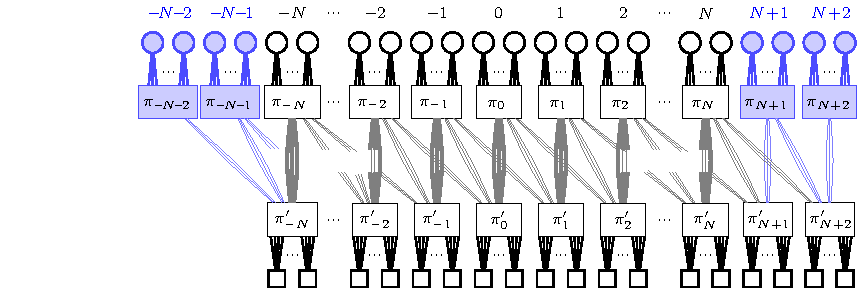
\includegraphics[width=0.9\textwidth]{./Figures/SC/spatially-coupled-ensemble.pdf}
\begin{center}
  The video link comes here
  \end{center}
\end{frame}

\begin{frame}{Rate loss for finite $N$ and $w$}
\centering
\begin{tabular}{|c|c|c|c|}
  \hline
  SC-LDPC & Shannon & \textcolor{blue}{AWGN} & \textcolor{blue}{BSC} \\
  $(\ell,r,N,w)$ & $\texttt{h}^{\mathrm{Sh}}$  & $\hbp_{\mathrm{c}}$ & $\hbp_{\mathrm{c}}$  \\
  \hline
  $(3,6,10,3)$ & $0.5434$ & $0.4794$ & $0.4681$ \\
  $(3,6,20,3)$ & $0.5222$ & $0.4794$ & $0.4681$ \\
  $(3,6,30,3)$ & $0.5149$ & $0.4794$ & $0.4681$ \\
  \hline
  $(4,6,10,3)$ & $0.7245$ & $0.6645$ & $0.6633$ \\
  $(4,6,20,3)$ & $0.6963$ & $0.6645$ & $0.6633$ \\
  $(4,6,30,3)$ & $0.6866$ & $0.6645$ & $0.6633$ \\
  \hline
  $(5,6,10,3)$ & $0.9056$ & $0.8333$ & $0.8333$ \\
  $(5,6,20,3)$ & $0.8704$ & $0.8333$ & $0.8333$ \\
  $(5,6,30,3)$ & $0.8582$ & $0.8333$ & $0.8333$ \\
  \hline
\end{tabular}
\end{frame}
%%%%%---------------------------------------------------------------------------------------------------------------%%%%%%%%%%%%%%%

\begin{frame}{Pros \& Cons}
\begin{defn}{Pros}
\begin{itemize}
\item Significant improvment in thresholds
\vspace{0.25cm}
\item Achieves capacity under {\blue simple BP decoding} [KRU'11,KYMP'14]
\vspace{0.25cm}
\item {\blue Universality} - works for all channels models! 
\vspace{0.25cm}
\end{itemize}
\end{defn}

\begin{defn}{Cons}
\begin{itemize}
\item Need \textcolor{red}{large} blocklengths to leverage the gains
\end{itemize}
\end{defn}
\end{frame}
%%%%%---------------------------------------------------------------------------------------------------------------%%%%%%%%%%%%%%%

\section{SC-LDPC Lattices}
\subsection{Introduction to Lattices}

\begin{frame}\frametitle{Lattice}
\begin{defn}{Lattice}
Let $\mathbf{G}\in\mathbb{R}^{n\times k}$. An $n$-dimensional real lattice $\Lambda$ can be defined as
$$
\Lambda=\{\mbf{G}\mbf{z}, \mbf{z}\in\mbb{Z}^{k}\}
$$
\end{defn}
\onslide<2->
\begin{columns}
\column{0.45\textwidth}
Example:\[
\mathbf{G}= \left[ \begin{array}{cc}
1 & -1/2 \\
0 & \sqrt{3}/2 \end{array} \right]\]
\column{0.55\textwidth}
\centering
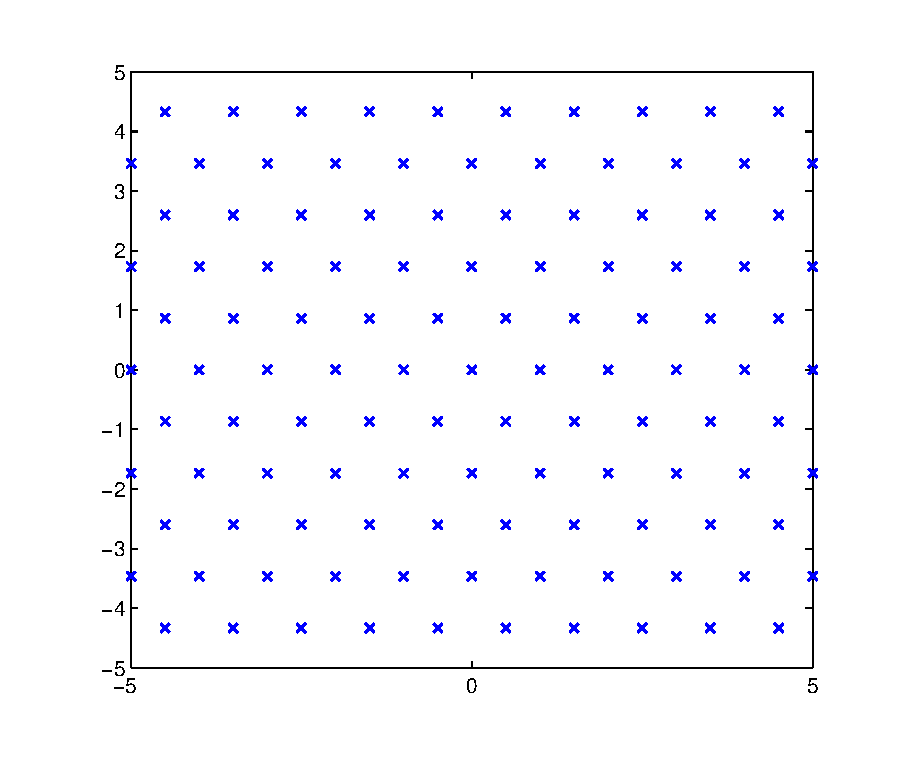
\includegraphics[width=2.4in]{./Figures/lattice.eps}
\end{columns}
\end{frame}

\begin{frame}\frametitle{Lattices and Lattice Codes}
\begin{defn}{Lattice}
Let $\mathbf{G}\in\mathbb{R}^{n\times k}$. An $n$-dimensional real lattice $\Lambda$ can be defined as
$$
\Lambda=\{\mbf{G}\mbf{z}, \mbf{z}\in\mbb{Z}^{k}\}
$$
\end{defn}
\vspace{-10pt}
\begin{itemize}
	\item Efficient structures for
	\begin{itemize}
	 		 \item {\blue Mathematics}: sphere packing and sphere covering problems
	   		 \item{\blue Information Theory}: channel coding \& quantization
    \end{itemize}
    \item Single user Gaussian channel - Erez and Zamir
	\item Coding with side information - Wyner-Ziv and Costa, Zamir, Erez and Shamai
	\item Secrecy - He and Yener
	\item Dirty multiple access channel - Philosof, Khisti, Erez and Zamir
\end{itemize}
\vspace{5pt}
	
``Lattices are everywhere" by Ram Zamir
\end{frame}

\begin{frame}\frametitle{Prior Work}
New perspectives for dealing with interference:
      \begin{itemize}
     		\item<1-> Interference alignment - Sridharan, Jafarian, Vishwanath and Jafar
			\item<2-> Compute-and-forward - Nazer \& Gastpar
			\item<2-> Physical layer network coding - Wilson et al, Nam et al
      \end{itemize}
			\vspace{2.5em}
			
	\begin{figure}
		\centering
		\only<1->{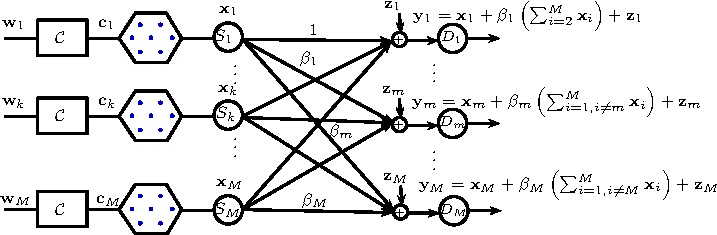
\includegraphics[width=4in]{IC_model_ISIT.pdf}}
	\end{figure}
\onslide<3->
\begin{itemize}
	\item Above schemes are all based on lattices {\blue good} for channel coding
\end{itemize}
\end{frame}

\begin{frame}\frametitle{Background on lattices}
\begin{defn}{Voronoi region}
The \textit{fundamental Voronoi region} $\mathcal{V}$ of a lattice, is the set of all points in $\mathbb{R}^n$ that are closest to the zero vector.
\vspace{-2mm}
\begin{align*}
\mc{V}\coleq \{\mbf{x}:\norm{\mbf{x-0}}\leq \norm{\mbf{x-c}} \quad\forall \mbf{c}\in\Lambda\}
\end{align*}
\end{defn}
\onslide<2->
\vspace{-3mm}
\centering
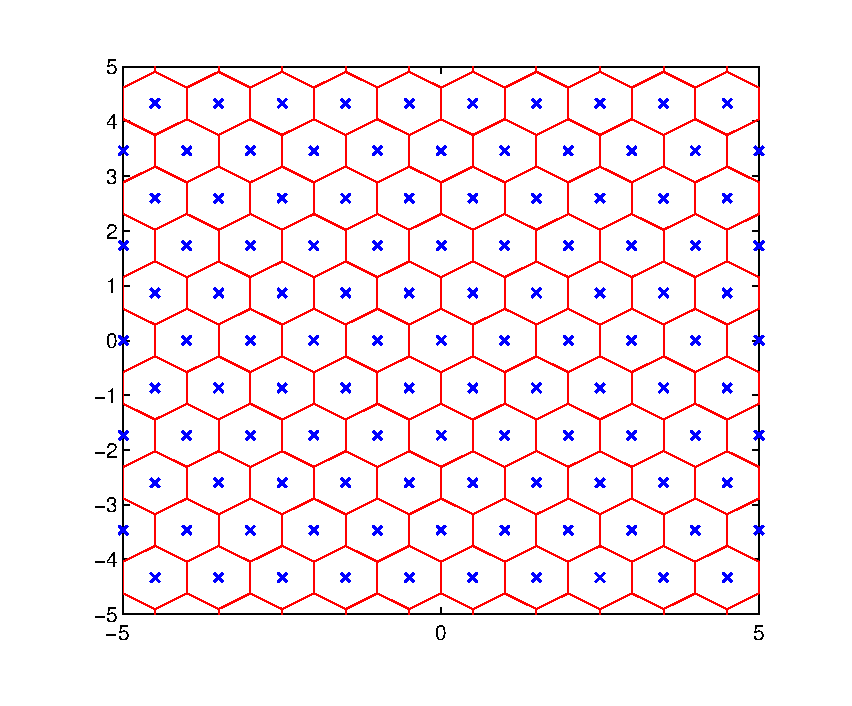
\includegraphics[width=0.5\textwidth]{./Figures/lattice_voronoi.eps}
\vspace{-3mm}
\onslide<3->
\begin{itemize}
\item Fundamental volume of $\Lambda$, $V(\Lambda)$: Vol($\mc{V}$)
\end{itemize}
\end{frame}

\begin{frame}\frametitle{Goodness of Lattices for Channel Coding}
\begin{itemize}
\item Let a lattice point $\lambda\in\Lambda$ is transmitted via AWGN channel of variance $\sigma^2$
\item Volume-to-noise ratio(VNR) of $\Lambda$:
\begin{align*}
\tx{VNR}\coleq\frac{V(\Lambda)^{2/n}}{2\pi e\sigma^2}
\end{align*}
\item $P(\Lambda,\sigma^2)\coleq \text{Pr}(d(\lambda,\lambda+\mbf{z})\geq d(\lambda',\lambda'+\mbf{z})) \tx{ for some } \mbf{\lambda'}\in\Lambda\ $
\end{itemize}
\onslide<2->
\begin{block}{Poltyrev Goodness for Channel Coding}
For any VNR$>1$ $\exists \{\Lambda_n\}$ such that $P(\Lambda_n,\sigma^2)\rightarrow 0$ as $n\rightarrow \infty$.
\end{block}
\begin{itemize}
	\item	{\blue \textit{Poltyrev-}good} lattices are at the core of such lattice coding schemes
\end{itemize}
\end{frame}  

\begin{frame}\frametitle{Objective}
\begin{defn}{Motivating questions}
	\begin{itemize}
		\item All the existing results were based on Construction-A.
		\begin{itemize}
				\item Linear codes over \alert{increasing field sizes} and their ML decoding 
		\end{itemize}
		\item<2-> Is this construction fundamental to good lattices?
		\item<2-> Can we work with just {\blue binary codes} under {\blue practical decoding} schemes?
	\end{itemize}
\end{defn}
\onslide<3->
\begin{defn}{Main Result}
\begin{itemize}
     \item Codes over \alert{$\mathbb{F}_{2}$ and BP decoding} suffice
	 \item<4-> We show existence of sequence of lattices that are \textit{Poltyrev}-good under BP
     \item<4-> Apply proposed lattices to {\blue Symmetric Interference Channel}
     \item<4-> Can be applied to other problems which adopt Construction-A lattices
\end{itemize}			
\end{defn}
\end{frame}

\begin{frame}\frametitle{Construction D with $L$ levels}
\begin{itemize}
    \item Barnes and Sloane '83, Forney, Chung and Trott '00, Yan, Ling, Wu ' 13
				 \vspace{0.5em}
	 \item Choose  $G_{1}\subseteq \ldots \subseteq G_{L}$ where $G_{l}$ is a gen matrix of code $\mc{C}_{l}$ over $\mathbb{F}_{2}$.
				 \vspace{.5em}
	\item<2->  $  \underline{\lambda} = \underline{w}_1 \mathbf{G}_1 + 2 \underline{w}_2 \mathbf{G}_2 \ldots +2^{L-1} \underline{w}_{L-1} \mathbf{G}_{L-1} +2^{L}\mathbb{Z}^{N} \in \Lambda$
\end{itemize}
				\vspace{0.2in}
    \begin{columns}[t]      
 	      \begin{column}{0.6\textwidth}
			\onslide<2->	{
            \begin{figure}
			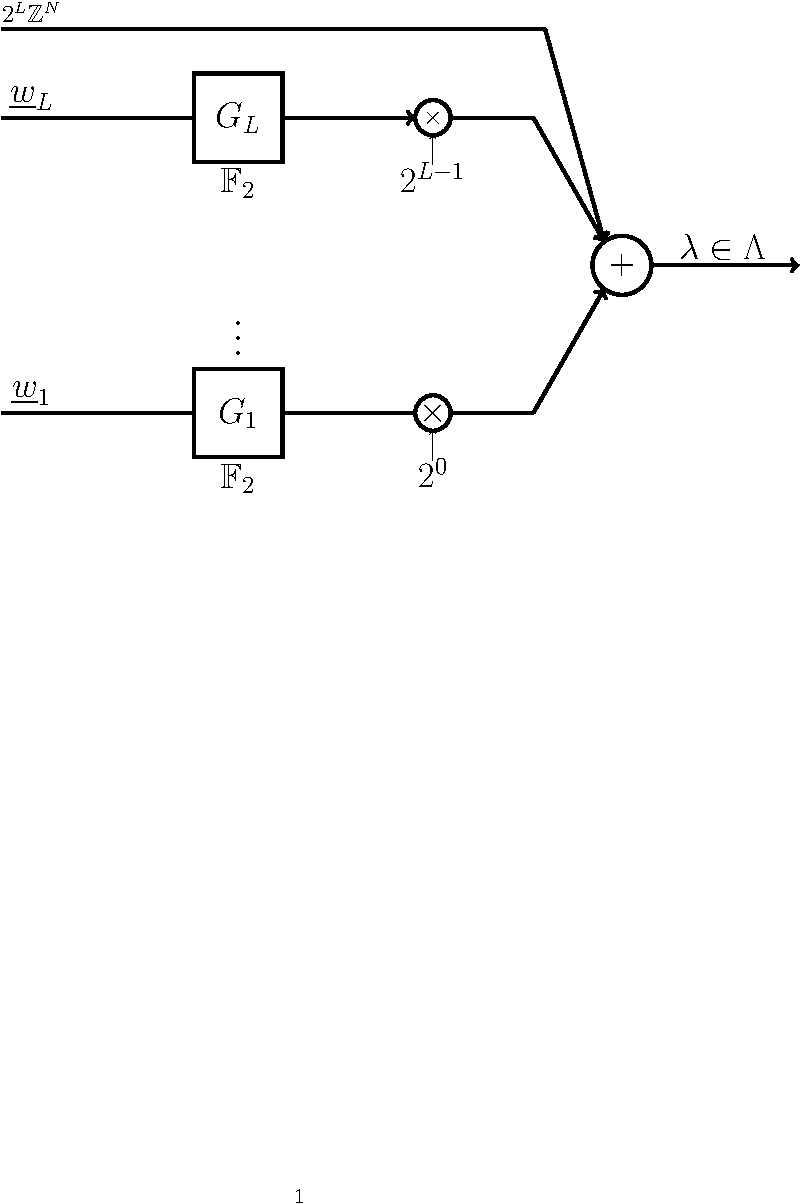
\includegraphics[width=2.5in]{lattice_Constr_D1.pdf}
            \end{figure}
            			}
        \end{column}

\begin{column}{0.39\textwidth}
	\begin{figure}
\only<1->{\resizebox{\columnwidth}{!}{
\begin{centering}
%\documentclass{article}
%\usepackage{graphicx,psfrag,epsfig,epsf,latexsym,hhline,amsmath,amssymb,multirow}
%\usepackage[usenames,dvipsnames]{pstricks}
%\usepackage{pst-plot}
%\usepackage{pstricks-add}
%\usepackage{color}
%\usepackage{stmaryrd}
%\usepackage{makecell}
%
%\interdisplaylinepenalty=2500
%\usepackage{graphicx}
%\usepackage{amsthm}
%\usepackage{footnote}
%\usepackage{blindtext}
%\usepackage{etoolbox}
%
%\usepackage{tikz}
%\usepackage{pgfplots}
%\usepgflibrary{shapes}
%\usetikzlibrary{matrix,positioning}
%\usetikzlibrary{decorations.pathreplacing}
%\usetikzlibrary{arrows,shapes,chains,matrix,positioning,scopes,patterns	}
%\pgfplotsset{compat=newest}
%\pgfplotsset{plot coordinates/math parser=false}
%
%\begin{document}

\begin{tikzpicture}
\def \offs{0.2in};

\matrix(mymatrix)[matrix of math nodes, left delimiter={[},right delimiter={]}]
	{
              \cdots & g_{L} & \cdots \\
              \cdots & \vdots & \cdots \\
%						\hline
              \cdots & g_{k_2} & \cdots \\
              \cdots & \vdots & \cdots \\
%						\hline
              \cdots & g_{k_1} & \cdots \\
              \cdots & \vdots & \cdots \\
              \cdots & g_2 & \cdots \\
              \cdots & g_1 & \cdots \\
	};        
\coordinate (la) at (mymatrix-1-1.north west);	
\coordinate (ra) at (mymatrix-1-3.north east);	

\coordinate (lb) at (mymatrix-2-1.south west);	
\coordinate (rb) at (mymatrix-2-3.south east);	

\coordinate (lc) at (mymatrix-4-1.south west);	
\coordinate (rc) at (mymatrix-4-3.south east);	

\coordinate (ld) at (mymatrix-8-1.south west);	
\coordinate (rd) at (mymatrix-8-3.south east);	


  \node (la_left)  [left = \offs of la]    {};    %Left coordinate outside the matrix for the 1st extended hline
  \node (ra_right)  [right = \offs of ra]    {};    %Right coordinate outside the matrix for the 1st extended hline
  \node (lb_left)  [left = \offs of lb]    {};    %Left coordinate outside the matrix for the 1st extended hline
  \node (rb_right)  [right = \offs of rb]    {};    %Right coordinate outside the matrix for the 1st extended hline
  \node (lc_left)  [left = \offs of lc]    {};    %Left coordinate outside the matrix for the 1st extended hline
  \node (rc_right)  [right = \offs of rc]    {};    %Right coordinate outside the matrix for the 1st extended hline
  \node (ld_left)  [left = \offs of ld]    {};    %Left coordinate outside the matrix for the 1st extended hline
  \node (rd_right)  [right = \offs of rd]    {};    %Right coordinate outside the matrix for the 1st extended hline

  \node (la_left_left)  [left = \offs of la_left]    {};    %Left coordinate outside the matrix for the 1st extended hline
  \node (ra_right_right)  [right = \offs of ra_right]    {};    %Right coordinate outside the matrix for the 1st extended hline
   \node (rd_right_right)  [right = \offs of rd_right]    {};    %Right coordinate outside the matrix for the 1st extended hline

%The two hlines in the Matrix
\draw[black,thick] (lb_left) -- (rb_right);
\draw[black,thick] (lc_left) -- (rc_right);


\draw [decorate,thick,decoration={brace,amplitude=4pt,mirror},xshift=5pt,yshift=0pt]
([xshift=-20pt]lc_left) -- ([xshift=-20pt]ld_left) node [black,midway,xshift=-10pt]{\small $\text{G}_{1}$};

\draw [decorate,thick,decoration={brace,amplitude=4pt},xshift=-10pt,yshift=0pt](rb_right) -- (rd_right) node [black,midway,xshift=15pt]{\small $\text{G}_{2}$};

\node [right= 0.5ex of rc_right] {$\cdots$};

\draw [decorate,thick,decoration={brace,amplitude=4pt},xshift=-10pt,yshift=0pt](ra_right_right) -- (rd_right_right) node [black,midway,xshift=15pt]{\small $\text{G}_{L}$};

%\draw [decorate,thick,decoration={brace,amplitude=4pt,mirror},xshift=-0.5in,yshift=0pt]
%(lb_left) -- (ld_left) node [black,midway,xshift=-19pt]{\small $\text{G}_{2}$};

 \end{tikzpicture}
%\end{document}
\end{centering}
}
}
	\end{figure}
\end{column}
    \end{columns}    
\end{frame}


\begin{frame}\frametitle{Multi-Level Decoding(Successive Cancellation) }
      \begin{itemize}
        \item $\underline{y} = \boxed{\underline{w}_1 \mathbf{G}_1 + 2 \underline{w}_2 \mathbf{G}_2 \ldots +2^{L-1} \underline{w}_{L-1} \mathbf{G}_{L-1} +2^{L}\mathbb{Z}^{N}} + \underline{n}$
         \vspace{0.05in}	
         \onslide<2->
         \item $\underline{y}$ mod 2 = $ \left[\,\underline{w}_1 \mathbf{G}_1 + \underline{n}\,\right] $ mod 2 = $\underline{w}_1 \odot \mathbf{G}            _1 + \boxed{\underline{n} \mod 2}$
         \vspace{0.05in}
		\item Decode $\underline{w}_1$, reconstruct $\underline{w}_1 \mathbf{G}_1$ and subtract from $\underline{y}$
         \vspace{0.2in}
    \end{itemize}
            \begin{figure}
					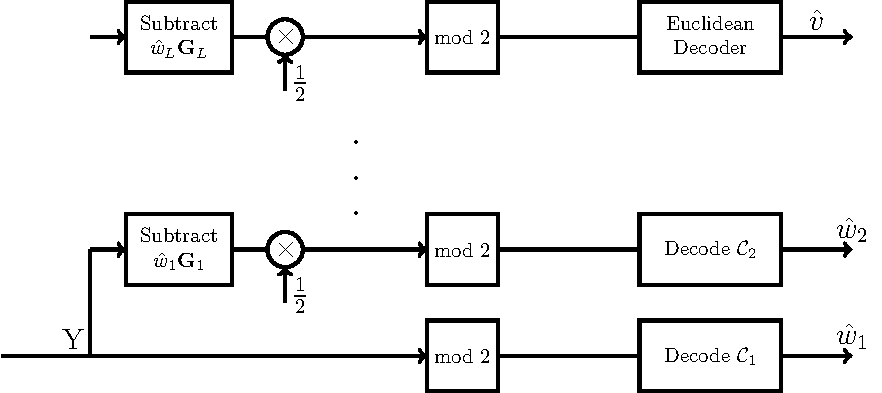
\includegraphics[width=0.7\textwidth]{multi_stage_decode.pdf}
            \end{figure}
	\end{frame}


\begin{frame}
%        \begin{theorem}[Forney, Trott \& Chung]
%            For an AWGN channel with noise variance $\sigma^{2}$ per dimension, there exists a Construction D lattice based on binary linear codes $\mc{C}_{1}\subseteq \mc{C}_{2}\ldots \subseteq \mc{C}_{r}$ such that the Volume-to-Noise(VNR) ratio is arbitrarily close to $1$ and the probability of error is arbitrarily small.
%       \end{theorem}
        \begin{theorem}[Forney, Trott \& Chung]
There exists a sequence of Construction D lattices based on $\mc{C}_{1}\subseteq \mc{C}_{2}\ldots \subseteq \mc{C}_{L}$ such that the VNR $\rightarrow 1$ and the $Pr(\lambda,\sigma^{2})\rightarrow 0$.
       \end{theorem}

\begin{itemize}
\item Take $L$ large enough.
\item It's sufficient that $\mc{C}_{i}$ at each level is capacity achieving for the mod-2 AWGN channel.
\end{itemize}
\pause
\vspace{0.4in}
Objective:
\begin{itemize}
\item Capacity achieving nested code constructions, preferably under BP decoding.
\end{itemize}
\end{frame}

\subsection{Proposed Lattice Construction}
\begin{frame}\frametitle{Proposed Nested Spatially-Coupled LDPC Ensemble}
    \begin{enumerate}
        \item<1-> Begin with a $(d_v^1,d_c)$ SC LDPC code. For ex, $(d_v^1=3,d_c=6,L=3,w=2)$. 
        \item<1-> Group check nodes into type $\mathcal{T}_k$, $k\in\{1,\ldots,d_v^1\}$
         \vspace{2pt}
        \item<2-> Remove all check nodes of type $\mathcal{T}_1,\ldots,\mathcal{T}_{d_v^1-d_v^2}$. Ex: $(d_{v}^{2}=2,6)$ sup-code.
                 \vspace{2pt}
        \item<3-> Results in a super-code that is a $(d_v^2,d_c)$ SC LDPC code.
    \end{enumerate}
    \vspace{0.15in}
    \begin{figure}
        \begin{center}
 	        \only<1>{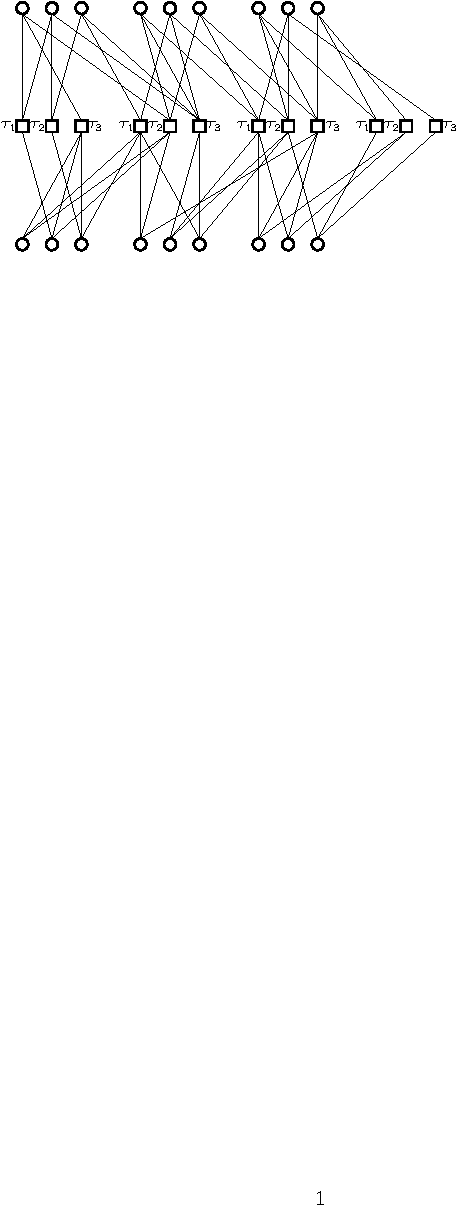
\includegraphics[width=3.2in]{Basegraph_ISIT1.pdf}}
         \only<2>{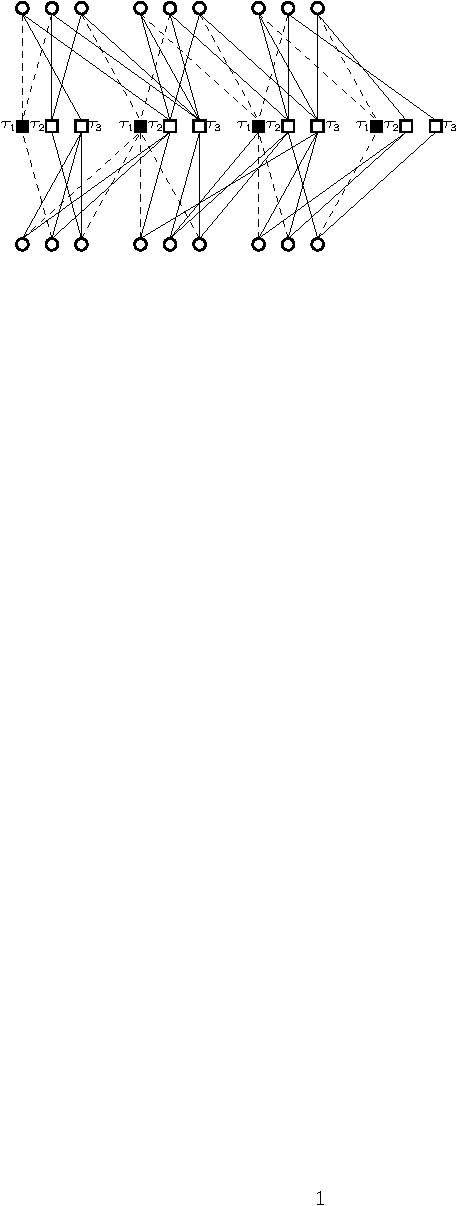
\includegraphics[width=3.2in]{Basegraph_ISIT2.pdf}}
         \only<3>{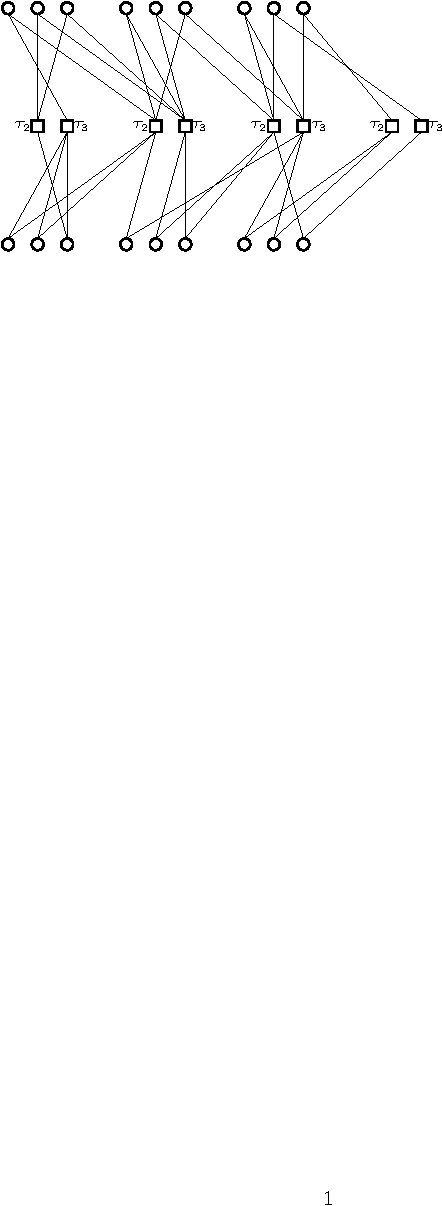
\includegraphics[width=3.1in]{Basegraph_ISIT3.pdf}}
        \end{center}
    \end{figure}
\end{frame}
         
\begin{frame}\frametitle{Lattice Design based on the proposed Nested SC LDPC ensemble}
\begin{enumerate}
\item For a given $\sigma$, compute the capacity of the mod-2 AWGN channel at each level:
		$$
         \underline{y_{i}}= \underline{w}_i \mathbf{G}_i +\frac{1}{2^{i-1}} \underline{n}\mod 2=\underline{w}_i \odot \mathbf{G}_i + \boxed{\frac{1}{2^{i-1}}\underline{n} \mod 2}
         $$
         \vspace{0.08in}

\item Fix check node degree $d_{c}$. Choose $d_{v}^{1},\ldots ,d_{v}^{r}$ such that the rate of the code at each level is arbitrarily close to the capacity at the respective level.
\end{enumerate}
\pause
\begin{lemma}\label{lemma:nested_G}
    Given nested binary linear codes $\mc{C}_{1}\subseteq \mc{C}_{2}\subseteq\ldots \subseteq\mc{C}_{r}$ there exists nested generator matrices for these codes.
\end{lemma}
\end{frame}

\subsection{Poltyrev Goodness}
\begin{frame}\frametitle{Proposed Ensemble is Capacity achieving}
\begin{theorem}
Each code ensemble in the proposed nested Spatially-Coupled LDPC ensemble is capacity achieving. 
\end{theorem}    
\begin{proof}
\begin{itemize}
        \item Each derived protograph has the same spatially coupled structure.
        \item Show that the mod 2 AWGN channel is BMS.
        \item The proof follows from [KRU'12] \& [KYMP'13]'s  results.
    \end{itemize}
\end{proof}
\end{frame}

\begin{frame}\frametitle{Proposed Lattices are Poltyrev-Good}
\begin{theorem}
There exists a sequence of SC LDPC lattices with VNR$(\Lambda,\sigma^{2})\rightarrow 1$ for which, under multistage BP decoding, $\mbb{E}\left[P(\lambda,\sigma^{2})\right]\rightarrow 0$ as $w,L,M  \rightarrow \infty$.
\end{theorem}    
\begin{proof}
\begin{itemize}
\item The proposed nested ensemble achieve capacity.
\item Follows from Forney's result.
\end{itemize}

\end{proof}
\vspace{0.3in}
\pause
\begin{itemize}
        \item {\blue Binary codes} and more importantly {\blue practical BP decoding} suffices. 
        \item Practically we observe that {\blue two levels} of coding gets you lattices very close to Poltyrev limit.
    \end{itemize}
\end{frame}
	
\begin{frame}\frametitle{Design Example of Poltyrev-Good Lattice}
Target error probability $P(2^L\Z^n,\sigma_{L}^2)=10^{-4}$ in the uncoded level $\implies\sigma_{L}=0.08$
\onslide<2->
\begin{enumerate}
\item  Capacities for the mod 2 AWGN  channel for respective levels: 
\vspace{0.1in}
\begin{center}
\begin{tabular}{| c | c | c | c | }
\hline
 & Level L-1   &  Level L-2  & Level L-3 \\
\hline 
$\sigma_{\text{eff}}$ & 0.16   &  0.32  & 0.64 \\ \hline
 Cap                           &  0.99 & 0.57 & 0.02 \\   \hline
 (14,30) (3,30)         &  0.9 & 0.533 & 0 \\   \hline
\end{tabular}
\end{center}
\onslide<3->
\vspace{0.1in}
\item Fix L=3 and use $(3,30)$, $(14,30)$ nested SC-LDPC codes.
\begin{itemize}
\item Note $P(4\Z^n,\sigma^2)\approx nP(4\Z,\sigma^2)$
\item We fix $n=2\times 10^5$
\end{itemize}
\vspace{0.07in}
\begin{center}
\begin{tabular}{c c c c c c c}
\hline  \hline
$(d_{c},d_{v}^{1},d_{v}^{2})$ &(L,w)& $P(4\Z,\sigma^{2})$ & $\sigma_{\text{max}}$ &$\text{VNR}$ &$\text{VNR}_{\text{rate-loss}}$\\
\hline
(30,14,3) & (32,4) & $5 \times 10^{-10}$ & 0.3184 & 1.02dB & 1.347dB \\
\onslide<4->
(60, 26, 3)& (72, 12)& $5 \times 10^{-10}$ & 0.3200 &0.482dB & 0.927dB\\
(60, 27, 3)& (64, 9)& $5 \times 10^{-10}$  &  0.3203 & 0.57dB & 0.951dB\\
%(60, 42, 3)& (80, 16)& $1 \times 10^{-6}$ & 0.4020 & 0.106dB &0.952dB\\
\end{tabular}
\end{center}
\end{enumerate}
\end{frame}

\begin{frame}\frametitle{Alternate Nested SC LDPC ensemble}
\begin{itemize}
		\item<1-> Derive a lower rate code by ``splitting the checks"
					\vspace{2pt}
		\item<1-> Consider a $(3,8)$ code
					\vspace{2pt}
		\item<2-> Split each check into ``two" checks to derive a $(3,4)$ sub-code
					\vspace{2pt}
		\item<2-> Easy to prove that resulting code is from the $(3,4)$ SC LDPC ensemble
\end{itemize}
\vspace{0.3in}
    \begin{figure}
        \begin{center}
         \only<1>{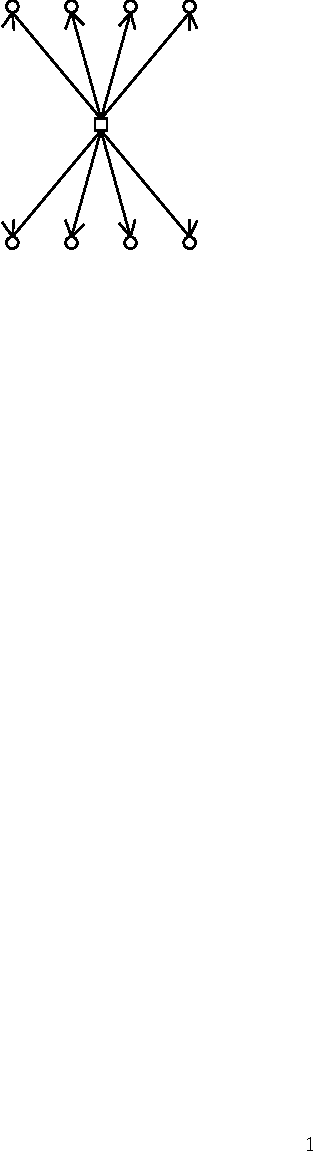
\includegraphics[width=2in]{Constr1_graph1.pdf}}
           \only<2>{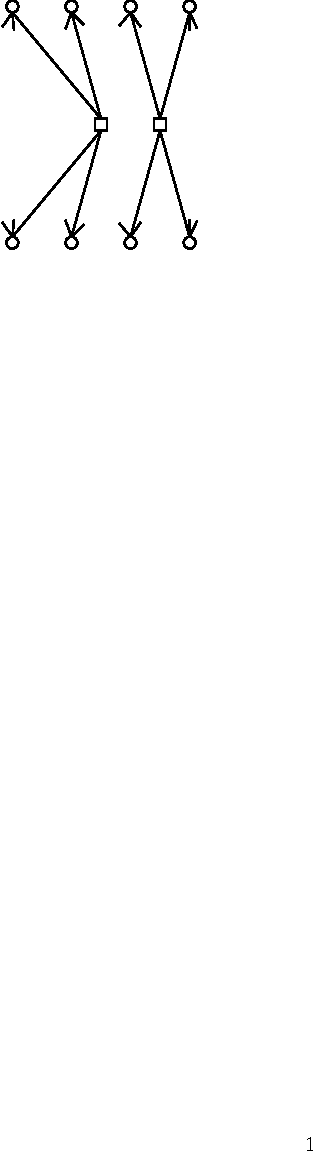
\includegraphics[width=2in]{Constr1_graph2.pdf}}
        \end{center}
    \end{figure}
\end{frame}

\begin{frame}\frametitle{Simulation Results}
\begin{figure}
\begin{center}
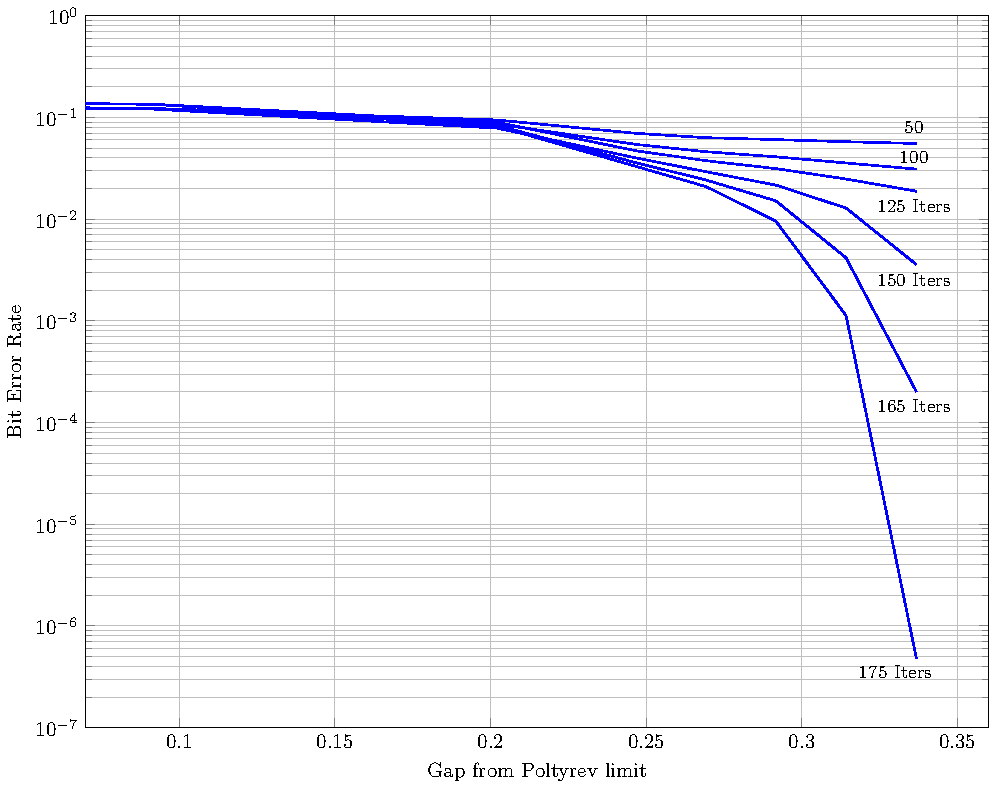
\includegraphics[width=0.6\textwidth]{BER_iters_4_72_9.pdf}
\end{center}
\end{figure}
\onslide<2->{Note that the Block Error Probability is $10^{-4}$ at uncoded level.}
\end{frame}

\subsection{Symmetric Interference Channel}
\begin{frame}\frametitle{3-User Symmetric Interference Channel}
	\begin{figure}
	\centering
    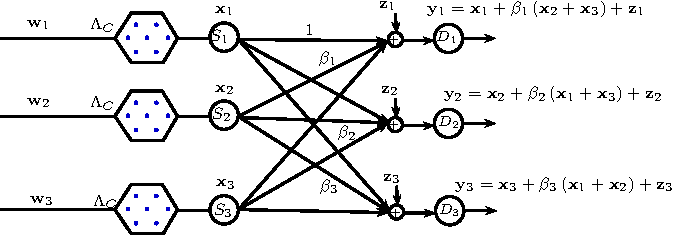
\includegraphics[width=4in]{IC_model_ISIT_3user.pdf}
	\end{figure}
\pause
\begin{itemize}
\item $\mathbf{x}_{i}\in \Lambda_{C}\defeq \Lambda \cap \mathbb{Z}_{4}^{N}$ is transmitted.
\vspace{0.2in}
\end{itemize}
\end{frame}


\begin{frame}\frametitle{Symmetric Interference Channel - Decoding Sums }
 Interference at Destination 1:
\begin{align*}
 \mathbf{x}_{2}+\mathbf{x}_{3}&= (\underline{w}_2^1+\underline{w}_3^1) \mathbf{G}_1 + 2 (\underline{w}_2^2+\underline{w}_3^2) \mathbf{G}_2 + 4\mathbf{k}_{23}\\
& = (\underline{w}_2^1 \oplus \underline{w}_3^1) \mathbf{G}_1 + 2 (\underline{c}_{23}^{1} \oplus \underline{w}_2^2 \oplus \underline{w}_3^2) \mathbf{G}_2 + 4(\underline{c}_{23}^{2} +\mathbf{k}_{23})\mathbf{Z}_{}
\end{align*}

where the carry overs are

\begin{align*}
& \underline{c}_{23}^{1}=0.5\left(\underline{w}_{1}^{1}+\underline{w}_{1}^{2}-\underline{w}_{1}^{1}\oplus\underline{w}_{1}^{2}\right), \\
& \underline{c}_{23}^{2}=0.5\left(\underline{c}_{23}^{1}+\underline{w}_{2}^{1}+\underline{w}_{2}^{2}-\underline{c}_{23}^{1}\oplus\underline{w}_{2}^{1} \oplus \underline{w}_{2}^{2}\right)
\end{align*}
%are carryovers from first and second levels respectively.
%and $\mathbf{k}_{23}=\mathbf{k}_{2}+\mathbf{k}_{3}+\sum_{1}^{k_{2}}c_{2i}\mathbf{g}_{i}\in\Z^{n}$. 
\begin{columns}
        \begin{column}{0.47\textwidth}
            \begin{figure}
               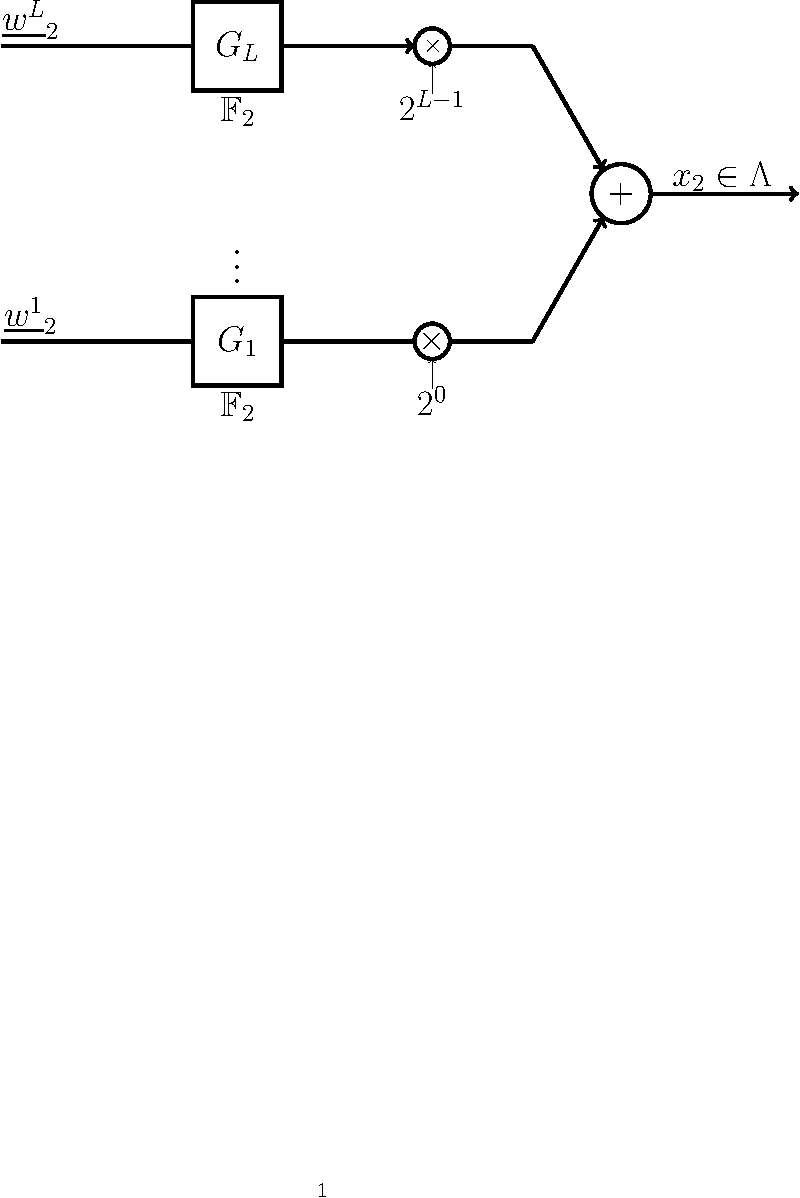
\includegraphics[width=2in]{lattice_Constr_D1_user1.pdf}
            \end{figure}
        \end{column}
        \begin{column}{0.47\textwidth}
            \begin{figure}
                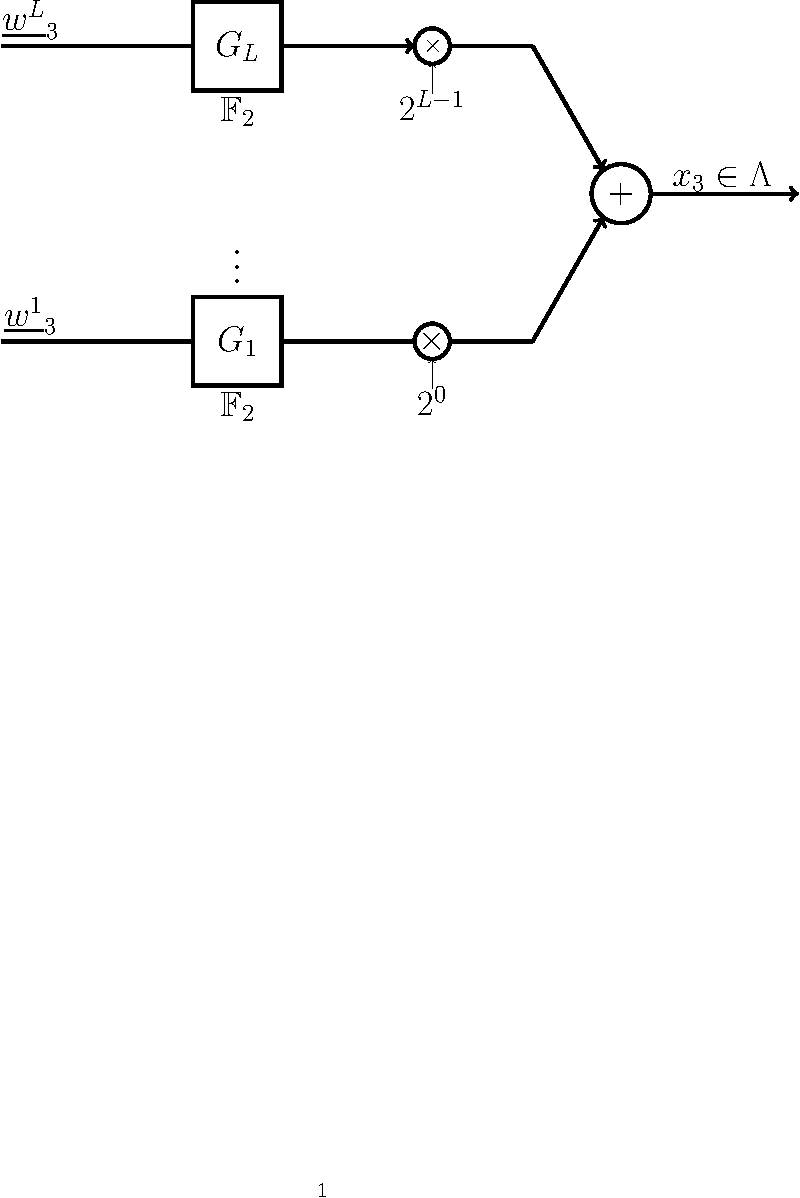
\includegraphics[width=2in]{lattice_Constr_D1_user2.pdf}
            \end{figure}
        \end{column}
\end{columns}
\end{frame}


\begin{frame}\frametitle{Achievable Information Rates}
    \begin{figure}
        \begin{center}
            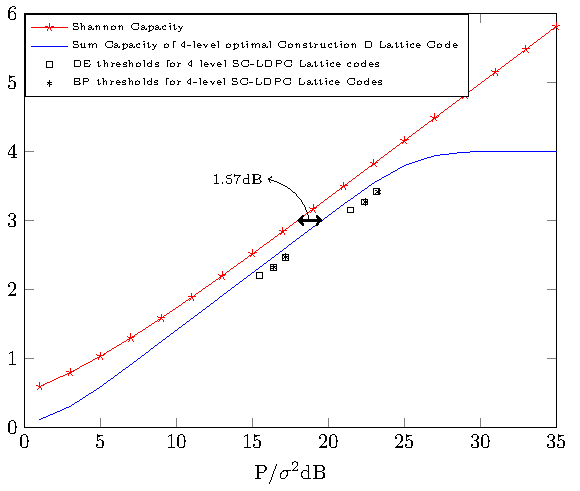
\includegraphics[width=3.5in]{ShapingLoss_Final_CTW.pdf}
        \end{center}
    \end{figure}
\end{frame}

\begin{frame}\frametitle{Concluding Remarks}
    \begin{itemize}
        \item Multilevel constructions - efficient ways to decode integer combinations
               \vspace{5pt}
        \item Need capacity achieving nested codes
                \vspace{5pt}
        \item Multilevel construction is provably good under message passing decoding
               \vspace{5pt}
               \pause
        \item Coding schemes based on \alert{binary codes and iterative decoding} suffice
    \end{itemize}
\end{frame}

\section{Side-Information Problems}
\subsection{Gelfand-Pinsker \& Wyner-Ziv}
\begin{frame}{Lossy Source Coding Problem}
  \centering{$X^n=(X_1,\cdots,X_n)$, $X_i \sim \mathsf{Bernoulli}(\frac{1}{2})$ \\ 
  \vspace{0.3cm}
	Binary code $\mathcal{C}=(n,k)$, rate $R=k/n$}
  \begin{block}{Lossy Source Coding}<2->
    \begin{columns}
      \column{0.55\textwidth}
      \begin{itemize}
      \item<2-> Compress $X^n$ to $\hat{X}^n \in \mathcal{C}$
      \item<2-> \textcolor{blue}{Min.~Hamming distortion}
        \begin{align*}
          D=\frac{1}{n} \sum_{i=1}^n \expt \abs{X_i-\hat{X}_i}
        \end{align*}
   \vspace{-4mm}
      \item<3-> Rate-Distortion theory: \vspace{-0.15cm}
        \begin{align*}
          R > 1 - h(D)
        \end{align*}
        \vspace{-7mm}
      \item<3-> $h(\cdot)$ is binary entropy function
        \small{
          \begin{align*}
            h(D)\!=\!-D \log_2 D \!-\! (1\!-\!D) \log_2 (1-D)
          \end{align*}
        }
      \end{itemize}
      \column{0.45\textwidth}<3->
      \setlength\tikzheight{3cm} 
      \setlength\tikzwidth{3.5cm} 
      \centering{\begin{tikzpicture}
  \begin{axis}[%
    font=\small,
    scale only axis,
    width=\tikzwidth,
    height=\tikzheight,
    xmin=0, xmax=0.5,
    ymin=0, ymax=1,
    xlabel={Distortion $D$},
    ylabel={Rate $R$},
    xmajorgrids,
    ymajorgrids]

    \filldraw[fill=black!30,draw=black]
    (axis description cs:0.0000,1.0000) -- 
    (axis description cs:0.0200,0.9192) -- 
    (axis description cs:0.0400,0.8586) -- 
    (axis description cs:0.0600,0.8056) -- 
    (axis description cs:0.0800,0.7577) -- 
    (axis description cs:0.1000,0.7136) -- 
    (axis description cs:0.1200,0.6726) -- 
    (axis description cs:0.1400,0.6341) -- 
    (axis description cs:0.1600,0.5978) -- 
    (axis description cs:0.1800,0.5635) -- 
    (axis description cs:0.2000,0.5310) -- 
    (axis description cs:0.2200,0.5001) -- 
    (axis description cs:0.2400,0.4706) -- 
    (axis description cs:0.2600,0.4426) -- 
    (axis description cs:0.2800,0.4158) -- 
    (axis description cs:0.3000,0.3902) -- 
    (axis description cs:0.3200,0.3657) -- 
    (axis description cs:0.3400,0.3423) -- 
    (axis description cs:0.3600,0.3199) -- 
    (axis description cs:0.3800,0.2985) -- 
    (axis description cs:0.4000,0.2781) -- 
    (axis description cs:0.4200,0.2585) -- 
    (axis description cs:0.4400,0.2398) -- 
    (axis description cs:0.4600,0.2220) -- 
    (axis description cs:0.4800,0.2050) -- 
    (axis description cs:0.5000,0.1887) -- 
    (axis description cs:0.5200,0.1733) -- 
    (axis description cs:0.5400,0.1585) -- 
    (axis description cs:0.5600,0.1445) -- 
    (axis description cs:0.5800,0.1313) -- 
    (axis description cs:0.6000,0.1187) -- 
    (axis description cs:0.6200,0.1068) -- 
    (axis description cs:0.6400,0.0956) -- 
    (axis description cs:0.6600,0.0851) -- 
    (axis description cs:0.6800,0.0752) -- 
    (axis description cs:0.7000,0.0659) -- 
    (axis description cs:0.7200,0.0573) -- 
    (axis description cs:0.7400,0.0493) -- 
    (axis description cs:0.7600,0.0420) -- 
    (axis description cs:0.7800,0.0352) -- 
    (axis description cs:0.8000,0.0290) -- 
    (axis description cs:0.8200,0.0235) -- 
    (axis description cs:0.8400,0.0185) -- 
    (axis description cs:0.8600,0.0142) -- 
    (axis description cs:0.8800,0.0104) -- 
    (axis description cs:0.9000,0.0072) -- 
    (axis description cs:0.9200,0.0046) -- 
    (axis description cs:0.9400,0.0026) -- 
    (axis description cs:0.9600,0.0012) -- 
    (axis description cs:0.9800,0.0003) -- 
    (axis description cs:1.0000,0.0000) -- 
    (axis description cs:1.0000,1.0000) -- cycle;
    
    \node at (axis description cs:0.6000,0.5000) {$R>1-h(D)$};
  \end{axis}
\end{tikzpicture}}
    \end{columns}
  \end{block}

\end{frame}

\begin{frame}{Side-Information Problems: Wyner-Ziv}
  \begin{center}
    \scalebox{0.5}{\begin{tikzpicture}
  [node distance=1cm,draw=black,thick, >=stealth']

  \def \reclen {3}
  \def \linelen {2}
  \def \recwid {0.75}

  \draw[->] (0,0) -- (0+\linelen,0);
  \draw (0+\linelen,\recwid) rectangle (0+\linelen+\reclen,-\recwid);
  \draw[->] (0+\linelen+\reclen,0) -- (0+\linelen+\reclen+\linelen,0);
  \draw (0+\linelen+\reclen+\linelen,\recwid) rectangle (0+\linelen+\reclen+\linelen+\reclen,-\recwid);
  \draw[->] (0+\linelen+\reclen+\linelen+\reclen,0) -- (0+\linelen+\reclen+\linelen+\reclen+\linelen,0);
  \draw (0+\linelen+\reclen+\linelen+\reclen+\linelen,\recwid) rectangle (0+\linelen+\reclen+\linelen+\reclen+\linelen+\reclen,-\recwid);

  \draw[->] (0.5*\linelen,0) -- (0.5*\linelen,-2) -- (1.5*\linelen+\reclen,-2);
  \draw (1.5*\linelen+\reclen,-2+\recwid) rectangle (2.5*\linelen+2*\reclen,-2-\recwid);
  \draw[->] (2.5*\linelen+2*\reclen,-2) -- (2*\linelen+2*\reclen+\linelen+0.5*\reclen,-2) -- (2*\linelen+2*\reclen+\linelen+0.5*\reclen,-\recwid);

  \node at (\linelen+0.5*\reclen,0.5*\recwid) {\Large{Encoder}};
  \node at (\linelen+0.5*\reclen,-0.5*\recwid) {\Large{$\mathcal{C}$}};

  \node at (2*\linelen+1.5*\reclen,0.5*\recwid) {\Large{Channel}};
  \node at (2*\linelen+1.5*\reclen,-0.5*\recwid) {\Large{Rate $R$}};

  \node at (3*\linelen+2.5*\reclen,0.5*\recwid) {\Large{Decoder}};
  \node at (3*\linelen+2.5*\reclen,-0.5*\recwid) {\Large{$(Y,Z^n)$}};

  \node at (2*\linelen+1.5*\reclen,-2+0.5*\recwid) {\Large{Side-Information}};
  \node at (2*\linelen+1.5*\reclen,-2-0.5*\recwid) {\Large{$Z_i=X_i\oplus \mathsf{Ber}(\delta)$}};

  \node at (0.5*\linelen,0.5*\recwid) {\Large{$X^n$}};
  \node at (1.5*\linelen+\reclen,0.5*\recwid) {\Large{$f(\hat{X}^n)$}};
  \node at (2.5*\linelen+2*\reclen,0.5*\recwid) {\Large{$Y$}};
  \node at (3*\linelen+2.25*\reclen,-2+0.5*\recwid) {\Large{$Z^n$}};

\end{tikzpicture}

%%% Local Variables: 
%%% mode: latex
%%% TeX-master: "../talk"
%%% End: 
}
  \end{center}
  \begin{block}{Wyner-Ziv Formulation}<1->
    \begin{columns}
      \column{0.55\textwidth}
      \vspace{-3mm}
      \begin{itemize}
      \item<1-> \textcolor{red}{Side-information} $Z^n$ about $X^n$
      \item<1-> Decoder \textcolor{blue}{additionally} has $Z^n$
      \item<1-> Say $Z_i = X_i \oplus \mathsf{Ber}(\delta)$
      \item<2-> Wyner-Ziv theory:
        \begin{align*}
          R > l.c.e\{h(D*\delta)-h(D), (\delta,0)\}
        \end{align*}
      \item<2-> $D*\delta=D(1-\delta)+\delta(1-D)$
      \end{itemize}
      \column{0.45\textwidth}<2->
      \setlength\tikzheight{3cm} 
      \setlength\tikzwidth{3.5cm} 
      \centering{\begin{tikzpicture}

  \begin{axis}[%
    font=\small,
    scale only axis,
    width=\tikzwidth,
    height=\tikzheight,
    xmin=0, xmax=0.5,
    ymin=0, ymax=1,
    xlabel={Distortion $D$},
    ylabel={Rate $R$},
    xmajorgrids,
    ymajorgrids]

    \filldraw[fill=black!30,draw=black]
    (axis description cs:0.0000,0.8113) -- 
    (axis description cs:0.0200,0.7383) -- 
    (axis description cs:0.0400,0.6853) -- 
    (axis description cs:0.0600,0.6398) -- 
    (axis description cs:0.0800,0.5992) -- 
    (axis description cs:0.1000,0.5622) -- 
    (axis description cs:0.1200,0.5280) -- 
    (axis description cs:0.1400,0.4963) -- 
    (axis description cs:0.1600,0.4665) -- 
    (axis description cs:0.1800,0.4386) -- 
    (axis description cs:0.2000,0.4123) -- 
    (axis description cs:0.2200,0.3874) -- 
    (axis description cs:0.2400,0.3638) -- 
    (axis description cs:0.2600,0.3414) -- 
    (axis description cs:0.2800,0.3201) -- 
    (axis description cs:0.3000,0.2999) -- 
    (axis description cs:0.3200,0.2806) -- 
    (axis description cs:0.3400,0.2622) -- 
    (axis description cs:0.3600,0.2447) -- 
    (axis description cs:0.3800,0.2281) -- 
    (axis description cs:0.4000,0.2121) -- 
    (axis description cs:0.4200,0.1970) -- 
    (axis description cs:0.4400,0.1825) -- 
    (axis description cs:0.4600,0.1687) -- 
    (axis description cs:0.4800,0.1556) -- 
    (axis description cs:0.5000,0.1432) -- 
    (axis description cs:0.5200,0.1313) -- 
    (axis description cs:0.5400,0.1200) -- 
    (axis description cs:0.5600,0.1093) -- 
    (axis description cs:0.5800,0.0992) -- 
    (axis description cs:0.6000,0.0897) -- 
    (axis description cs:0.6200,0.0806) -- 
    (axis description cs:0.6400,0.0721) -- 
    (axis description cs:0.6600,0.0641) -- 
    (axis description cs:0.6800,0.0566) -- 
    (axis description cs:0.7000,0.0496) -- 
    (axis description cs:0.7200,0.0431) -- 
    (axis description cs:0.7400,0.0371) -- 
    (axis description cs:0.7600,0.0315) -- 
    (axis description cs:0.7800,0.0265) -- 
    (axis description cs:0.8000,0.0218) -- 
    (axis description cs:0.8200,0.0176) -- 
    (axis description cs:0.8400,0.0139) -- 
    (axis description cs:0.8600,0.0106) -- 
    (axis description cs:0.8800,0.0078) -- 
    (axis description cs:0.9000,0.0054) -- 
    (axis description cs:0.9200,0.0035) -- 
    (axis description cs:0.9400,0.0019) -- 
    (axis description cs:0.9600,0.0009) -- 
    (axis description cs:0.9800,0.0002) -- 
    (axis description cs:1.0000,0.0000) -- 
    (axis description cs:1.0000,1.0000) -- 
    (axis description cs:0.0000,1.0000) -- 
    cycle;

    \filldraw[fill=black!30,draw=black]
    (axis description cs:0.2000,0.4123) -- 
    (axis description cs:0.2200,0.3874) -- 
    (axis description cs:0.2400,0.3638) -- 
    (axis description cs:0.2600,0.3414) -- 
    (axis description cs:0.2800,0.3201) -- 
    (axis description cs:0.3000,0.2999) -- 
    (axis description cs:0.3200,0.2806) -- 
    (axis description cs:0.3400,0.2622) -- 
    (axis description cs:0.3600,0.2447) -- 
    (axis description cs:0.3800,0.2281) -- 
    (axis description cs:0.4000,0.2121) -- 
    (axis description cs:0.4200,0.1970) -- 
    (axis description cs:0.4400,0.1825) -- 
    (axis description cs:0.4600,0.1687) -- 
    (axis description cs:0.4800,0.1556) -- 
    (axis description cs:0.5000,0.1432) -- 
    (axis description cs:0.5200,0.1313) -- 
    (axis description cs:0.5400,0.1200) -- 
    (axis description cs:0.5600,0.1093) -- 
    (axis description cs:0.5800,0.0992) -- 
    (axis description cs:0.6000,0.0897) -- 
    (axis description cs:0.6200,0.0806) -- 
    (axis description cs:0.6400,0.0721) -- 
    (axis description cs:0.6600,0.0641) -- 
    (axis description cs:0.6800,0.0566) -- 
    (axis description cs:0.7000,0.0496) -- 
    (axis description cs:0.7200,0.0431) -- 
    (axis description cs:0.7400,0.0371) -- 
    (axis description cs:0.7600,0.0315) -- 
    (axis description cs:0.7800,0.0265) -- 
    (axis description cs:0.8000,0.0218) -- 
    (axis description cs:0.8200,0.0176) -- 
    (axis description cs:0.8400,0.0139) -- 
    (axis description cs:0.8600,0.0106) -- 
    (axis description cs:0.8800,0.0078) -- 
    (axis description cs:0.9000,0.0054) -- 
    (axis description cs:0.9200,0.0035) -- 
    (axis description cs:0.9400,0.0019) -- 
    (axis description cs:0.9600,0.0009) -- 
    (axis description cs:0.9800,0.0002) -- 
    (axis description cs:1.0000,0.0000) -- 
    (axis description cs:0.500,0.0000) -- 
    (axis description cs:0.2000,0.4123) -- 
    cycle;
    \node at (axis description cs:0.5,0.5) {$\delta=0.25$};
  \end{axis}
\end{tikzpicture}

%%% Local Variables: 
%%% mode: latex
%%% TeX-master: "../talk"
%%% End: 
}
    \end{columns}
  \end{block}
\end{frame}

\begin{frame}{Side-Information Problems: Gelfand-Pinsker}
  \begin{center}
    \scalebox{0.5}{\begin{tikzpicture}
  [yscale=0.8,node distance=1cm,draw=black,thick, >=stealth']

  \def \reclen {3}
  \def \linelen {2}
  \def \recwid {0.75}

  \draw[->] (-1,0) -- (-1+\linelen,0);
  \draw (0+\linelen-1,\recwid) rectangle (0+\linelen+\reclen-1,-\recwid);
  \node (sideinfnode) at (0+\linelen+\reclen+\linelen,0) {\Huge{$\oplus$}};
  \draw[->] (0+\linelen+\reclen-1,0) -- (sideinfnode);
  \draw[->] (sideinfnode) -- (0+\linelen+\reclen+\linelen+\linelen,0);
  \node (znlabel) at (0+\linelen+\reclen+\linelen,3*\recwid) {\Large{$Z^n$}};
  \draw[->] (znlabel) -- (sideinfnode);
  \draw[->] (sideinfnode) -- (0+\linelen+\reclen+\linelen,-3*\recwid) -- (\linelen+0.5*\reclen-1,-3*\recwid) -- (\linelen+0.5*\reclen-1,-\recwid);
  \draw (0+\linelen+\reclen+\linelen+\linelen,\recwid) rectangle (0+\linelen+\reclen+\linelen+\linelen+\reclen,-\recwid);
  \draw[->] (0+\linelen+\reclen+\linelen+\linelen+\reclen,0) -- (0+\linelen+\reclen+\linelen+\linelen+\reclen+0.5*\linelen,0);
  \draw (0+\linelen+\reclen+\linelen+\reclen+\linelen+0.5*\linelen,\recwid) rectangle (0+\linelen+\reclen+\linelen+\reclen+\linelen+\reclen+1.5*\linelen,-\recwid);

  \node at (\linelen+0.5*\reclen-1,0.5*\recwid) {\Large{Codebook}};
  \node at (\linelen+0.5*\reclen-1,-0.5*\recwid) {\Large{$\mathcal{C}(n,k)$}};

  \node at (3*\linelen+1.5*\reclen,0.5*\recwid) {\Large{Channel}};
  \node at (3*\linelen+1.5*\reclen,-0.5*\recwid) {\Large{$W^n \sim \mathsf{Ber}(\delta)$}};

  \node at (4*\linelen+2.5*\reclen,0.5*\recwid) {\Large{Decoder}};
  \node at (4*\linelen+2.5*\reclen,-0.5*\recwid) {\Large{$Y^n=X^n\oplus Z^n \oplus W^n$}};

  \node at (0.5*\linelen-1,0.65*\recwid) {\Large{$M^k$}};
  \node at (0.5*\linelen-1,-0.65*\recwid) {\Large{Rate $R$}};
  \node at (1.5*\linelen+\reclen-0.5,0.5*\recwid) {\Large{$X^n$}};
  \node at (1.5*\linelen+\reclen-0.5,-0.5*\recwid) {\large{$\mathrm{Weight}\leq p$}};

\end{tikzpicture}

%%% Local Variables: 
%%% mode: latex
%%% TeX-master: "../talk"
%%% End: 
}
  \end{center}
  \begin{block}{Gelfand-Pinsker Formulation}<2->
    \begin{itemize}
    \item<2-> Message $M^k$ encoded to $X^n \in \mathcal{C}$ with \textcolor{blue}{$\tfrac{1}{n} \sum_{i=1}^n \expt[X_i] \leq p \leq \frac{1}{2}$}
    \item<2-> Side-information $Z^n$ is available \alert{only at the encoder}
    \item<2-> The output at the decoder is
      \begin{align*}
        Y^n=X^n\oplus Z^n \oplus W^n, \quad \{W_i\} \sim \textsf{Ber}(\delta)
      \end{align*}
    \item<3-> Capacity region by Gelfand-Pinsker:
      \begin{align*}
        R < h(p) - h(\delta)
      \end{align*}
    \end{itemize}
  \end{block}
\end{frame}

\begin{frame}{Main Result}
  \begin{block}{Objective}<1->
    \begin{itemize}
    \item Construct {\blue low-complexity} coding schemes that achieve the \textcolor{blue}{complete rate regions} of Wyner-Ziv and Gelfand-Pinsker \vspace{0.1cm}
      \begin{itemize}
      \item Low-complexity encoding and decoding
      \end{itemize}
    \end{itemize}
  \end{block}
  \vspace{0.1cm}
  \begin{block}{Idea}<2->
    \begin{itemize}
    \item Wainwright et al.~used compound LDGM/LDPC codes with \alert{optimal encoding/decoding}\vspace{0.1cm}
    \item Message-passing algorithms have \alert{non-negligible gap}\vspace{0.1cm}
    \item<3-> Remedy via {\blue Spatial-Coupling}
      \begin{itemize}
      \item Channel coding in coupled compound codes (Kasai et al.)
      \item Lossy source coding with spatially-coupled LDGM (Aref et al.)
      \item Encoding with compound codes has additional challenges
      \end{itemize}
    \end{itemize}
  \end{block}
\end{frame}

\subsection{Compound LDGM/LDPC Codes}
\begin{frame}\frametitle{An $(\ell,r)$ LDGM Code}
\begin{columns}
\column{0.55\textwidth}
\begin{defn}{Generator Matrix}
\vspace{-3mm}
\centering
\begin{align*}
G=
\begin{pmatrix}
1 & 1 & 0 & 0 & 1 & 0\\
0 & 0 & 1 & 1 & 1 & 0\\
1 & 0 & 1 & 0 & 0 & 1\\
0 & 1 & 0 & 1 & 0 & 1  
\end{pmatrix}
\end{align*}
\begin{align*}
  \ell&=3 & r&=2
\end{align*}
\begin{align*}
\text{LDGM Code } \mc{C}=\{x: x=m\odot G\}
\end{align*}
\end{defn}
\column{0.45\textwidth}
\begin{defn}{Tanner Graph}
\centering
\vspace{1mm}
\scalebox{0.7}{\begin{tikzpicture}
  [
  node distance = 12mm, draw=black, thick, >=stealth',
  bitnode/.style={circle, inner sep = 0pt, minimum size = 3.5mm, draw=black},
  checknode/.style={rectangle, inner sep = 0pt, minimum size = 4mm, draw=black},
  ]
  
  \foreach \x in {1,2,...,4} {
    \node[bitnode] (b\x) at (\x,0) {$m_{\x}$};
  }

  \foreach \x in {1,...,6} {
    \node[checknode] (cc\x) at (\x-1,+2) {};
    \node[bitnode,fill=gray] (b1\x) at (\x-1,+3) {};
	\node[above] at (b1\x.north)  {$x_{\x}$};
    \draw[thin] (cc\x.north) -- (b1\x.south);
  }

  \draw[thin] (cc1) -- (b1);
  \draw[thin] (cc1) -- (b3);
  \draw[thin] (cc2) -- (b1);
  \draw[thin] (cc2) -- (b4);
  \draw[thin] (cc3) -- (b2);
  \draw[thin] (cc3) -- (b3);
  \draw[thin] (cc4) -- (b2);
  \draw[thin] (cc4) -- (b4);
  \draw[thin] (cc5) -- (b1);
  \draw[thin] (cc5) -- (b2);
  \draw[thin] (cc6) -- (b3);
  \draw[thin] (cc6) -- (b4);
  
  \draw[<->] (3.5,0.2) to [bend left=30] (4.5,0.45)  node [right] {\Large $\ell$};
  \draw[<->] (4.5,1.8) to [bend right=25] (5,1.45) node [right] {\Large $r$};



\end{tikzpicture}

%%% Local Variables: 
%%% mode: latex
%%% TeX-master: "../main"
%%% End: 
}
\end{defn}
\vspace{0.3cm}
\pause
$$ x_1=m_1\oplus m_3 \iff x_1\oplus m_1\oplus m_3=0 $$
\end{columns}
\end{frame}
%%%%%%%%%%%%----------------------------------------------------------------------------------%%%%%%%%%%%%%%%
\begin{frame}{Compound LDGM/LDPC Codes}
\begin{columns}
   \column{0.45\textwidth}
 \begin{center}
    \setlength\tikzheight{5cm}
    \setlength\tikzwidth{6cm}
    \scalebox{0.5}{\begin{tikzpicture}
  [
  node distance = 12mm, draw=black, thick, >=stealth',
  bitnode/.style={circle, inner sep = 0pt, minimum size = 5.5mm, draw=black},
  checknode/.style={rectangle, inner sep = 0pt, minimum size = 4mm, draw=black},
  bitnode2/.style={circle, inner sep = 0pt, minimum size = 4mm, draw=black, fill=black!50},
  ]
  
  \foreach \x in {1,2,...,9} {
    \node[bitnode2] (bb\x) at (\x-5,3) {};
  }

  \foreach \y in {1,2,...,9} {
    \node at (\y-5,3.5) {$x_{\y}$};
  }

  \foreach \x in {1,2,...,9} {
    \node[checknode] (c\x) at (\x-5,2) {};
    \draw[thin] (c\x) -- (bb\x);
  }

  \foreach \x in {1,2,...,6} {
    \node[bitnode] (b\x) at (1.2*\x-4.2,0) {$u_{\x}$};
  }

  \foreach \x in {1,...,4} {
    \node[checknode] (cc\x) at (5*\x/3-2.5-5/3,-2) {};
  }

  \draw[thin] (c1) -- (b4);
  \draw[thin] (c1) -- (b1);
  \draw[thin] (c2) -- (b1);
  \draw[thin] (c2) -- (b3);
  \draw[thin] (c3) -- (b3);
  \draw[thin] (c3) -- (b2);
  \draw[thin] (c4) -- (b1);
  \draw[thin] (c4) -- (b6);
  \draw[thin] (c5) -- (b2);
  \draw[thin] (c5) -- (b5);
  \draw[thin] (c6) -- (b5);
  \draw[thin] (c6) -- (b6);
  \draw[thin] (c7) -- (b3);
  \draw[thin] (c7) -- (b4);
  \draw[thin] (c8) -- (b5);
  \draw[thin] (c8) -- (b2);
  \draw[thin] (c9) -- (b4);
  \draw[thin] (c9) -- (b6);


  \draw[thin] (cc1) -- (b2);
  \draw[thin] (cc1) -- (b1);
  \draw[thin] (cc1) -- (b5);
  \draw[thin] (cc2) -- (b5);
  \draw[thin] (cc2) -- (b3);
  \draw[thin] (cc2) -- (b4);
  \draw[thin] (cc3) -- (b1);
  \draw[thin] (cc3) -- (b3);
  \draw[thin] (cc3) -- (b6);
  \draw[thin] (cc4) -- (b2);
  \draw[thin] (cc4) -- (b6);
  \draw[thin] (cc4) -- (b4);

  \draw[<->] (3.5,2) to [bend right=25] (4,1.5) node [right] {\Large $d_{c}$};
  \draw[<->] (2.25,0.1) to [bend left=30] (3.5,0.5) node [right] {\Large $d_{v}$};
  \draw[<->] (2.5,-0.1) to [bend right=30] (3.25,-0.5) node [right] {\Large $d'_{v}$};
  \draw[<->] (2,-2) to [bend left=25] (3,-1.5) node [right] {\Large $d'_{c}$};

  \node at (-4.5,2.5) {\Large $n$};
  \node at (-3.8,0) {\Large $m$};

  \node at (5*1/3-2.5-5/3,-2.5) {$s_1$};
  \node at (5*2/3-2.5-5/3,-2.5) {$s_2$};
  \node at (5*3/3-2.5-5/3,-2.5) {$0$};
  \node at (5*4/3-2.5-5/3,-2.5) {$0$};

  \draw[decorate,decoration={brace,amplitude=5pt,mirror}] (-2.8,-2.75) -- (-0.55,-2.75) node [midway,yshift=-0.5cm] {$\mathcal{P}_1$,  $|\mathcal{P}_1|=k$};
  \draw[decorate,decoration={brace,amplitude=5pt,mirror}] (3.33-2.8,-2.75) -- (3.33-0.55,-2.75) node [midway,yshift=-0.5cm]{$\mathcal{P}_2$,  $|\mathcal{P}_2|=k'$};
\end{tikzpicture}

%%% Local Variables: 
%%% mode: latex
%%% TeX-master: "../isit14"
%%% End: 
}
 \end{center}
   \column{0.55\textwidth}
    \begin{itemize}
    \item Codebook $\mathcal{C}(n,m-k-k')$ \vspace{0.1cm}
    \item \textcolor{blue}{Message constraints} \vspace{-0.2cm}
      \begin{align*}
        u_1\oplus u_2 \oplus u_5&=s_1, &  u_1\oplus u_3 \oplus u_6&=0
      \end{align*}
    \item Codeword $(x_1,\cdots,x_9)$: \vspace{-0.2cm}
      \begin{align*}
        x_1 &= u_1 \oplus u_4, & x_2 &= \cdots
      \end{align*}
    \end{itemize}
  \end{columns}
  \begin{block}{Key Properties}<2->
    \begin{itemize}
    \item Compound code is 
      \begin{itemize}
      \item a {\blue good source code} under optimal encoding
      \item a {\blue good channel code} under optimal decoding
      \end{itemize}
     \item LDGM code is 
       \begin{itemize}
       \item a {\blue good source code} under optimal encoding
       \item \textcolor{blue}{(side note)} LDGM code is \alert{not} a good channel code
       \end{itemize}
    \end{itemize}
  \end{block}
\end{frame}

\begin{frame}{Good Code}
  \begin{block}{``Good'' source code}
    \begin{itemize}
    \item Rate of the code is $R=1-h(D)+\varepsilon$
    \item When this code is used to \alert{optimally encode} $\mathsf{Ber}(\tfrac{1}{2})$ source
    \item The average Hamming \textcolor{blue}{distortion is at most $D$}
    \end{itemize}
  \end{block}
  \vspace{0.4cm}
  \onslide<2->
  \begin{block}{``Good'' channel code}
    \begin{itemize}
    \item Rate of the code is $R=1-h(\delta)-\varepsilon$
    \item When this code is used for channel coding on $\mathsf{BSC}(\delta)$
    \item Message est.~under \alert{optimal decoding} with \textcolor{blue}{error at most $\varepsilon$}
    \end{itemize}
  \end{block}
\end{frame}

 \begin{frame}{Coding Scheme: Wyner-Ziv}
   \vspace{-0.4cm}
   \begin{center}
     \scalebox{0.4}{\begin{tikzpicture}
  [node distance=1cm,draw=black,thick, >=stealth']

  \def \reclen {3}
  \def \linelen {2}
  \def \recwid {0.75}

  \draw[->] (0,0) -- (0+\linelen,0);
  \draw (0+\linelen,\recwid) rectangle (0+\linelen+\reclen,-\recwid);
  \draw[->] (0+\linelen+\reclen,0) -- (0+\linelen+\reclen+\linelen,0);
  \draw (0+\linelen+\reclen+\linelen,\recwid) rectangle (0+\linelen+\reclen+\linelen+\reclen,-\recwid);
  \draw[->] (0+\linelen+\reclen+\linelen+\reclen,0) -- (0+\linelen+\reclen+\linelen+\reclen+\linelen,0);
  \draw (0+\linelen+\reclen+\linelen+\reclen+\linelen,\recwid) rectangle (0+\linelen+\reclen+\linelen+\reclen+\linelen+\reclen,-\recwid);

  \draw[->] (0.5*\linelen,0) -- (0.5*\linelen,-2) -- (1.5*\linelen+\reclen,-2);
  \draw (1.5*\linelen+\reclen,-2+\recwid) rectangle (2.5*\linelen+2*\reclen,-2-\recwid);
  \draw[->] (2.5*\linelen+2*\reclen,-2) -- (2*\linelen+2*\reclen+\linelen+0.5*\reclen,-2) -- (2*\linelen+2*\reclen+\linelen+0.5*\reclen,-\recwid);

  \node at (\linelen+0.5*\reclen,0.5*\recwid) {\Large{Encoder}};
  \node at (\linelen+0.5*\reclen,-0.5*\recwid) {\Large{$\mathcal{C}$}};

  \node at (2*\linelen+1.5*\reclen,0.5*\recwid) {\Large{Channel}};
  \node at (2*\linelen+1.5*\reclen,-0.5*\recwid) {\Large{Rate $R$}};

  \node at (3*\linelen+2.5*\reclen,0.5*\recwid) {\Large{Decoder}};
  \node at (3*\linelen+2.5*\reclen,-0.5*\recwid) {\Large{$(Y,Z^n)$}};

  \node at (2*\linelen+1.5*\reclen,-2+0.5*\recwid) {\Large{Side-Information}};
  \node at (2*\linelen+1.5*\reclen,-2-0.5*\recwid) {\Large{$Z_i=X_i\oplus \mathsf{Ber}(\delta)$}};

  \node at (0.5*\linelen,0.5*\recwid) {\Large{$X^n$}};
  \node at (1.5*\linelen+\reclen,0.5*\recwid) {\Large{$f(\hat{X}^n)$}};
  \node at (2.5*\linelen+2*\reclen,0.5*\recwid) {\Large{$Y$}};
  \node at (3*\linelen+2.25*\reclen,-2+0.5*\recwid) {\Large{$Z^n$}};

\end{tikzpicture}

%%% Local Variables: 
%%% mode: latex
%%% TeX-master: "../talk"
%%% End: 
}
   \end{center}
   \vspace{-0.35cm}
   \begin{columns}
     \column{0.5\textwidth}
     \vspace{-0.5cm}
     \begin{center}
       \setlength\tikzheight{6cm}
       \setlength\tikzwidth{7cm}
       \scalebox{0.65}{\begin{tikzpicture}
  [
  node distance = 12mm, draw=black, thick, >=stealth',
  bitnode/.style={circle, inner sep = 0pt, minimum size = 5.5mm, draw=black},
  bitnodehidden/.style={circle, inner sep = 0pt, minimum size = 5.5mm, draw=white},
  checknode/.style={rectangle, inner sep = 0pt, minimum size = 4mm, draw=black},
  checknodehidden/.style={rectangle, inner sep = 0pt, minimum size = 4mm, draw=white},
  bitnode2/.style={circle, inner sep = 0pt, minimum size = 4mm, draw=black, fill=black!50},
  bitnode2hidden/.style={circle, inner sep = 0pt, minimum size = 4mm, draw=white, fill=white},
  ]

  \only<1>{

    \foreach \x in {1,2,...,9} {
      \node[bitnode2hidden] (bb\x) at (\x-5,3) {};
    }

    \foreach \y in {1,2,...,9} {
      \node[white] at (\y-5,4.5) {\Large{$x_{\y}$}};
    }

    \foreach \y in {1,2,...,9} {
      \node[white] at (\y-5,3.5) {\Large{$\hat{x}_{\y}$}};
    }

    \foreach \x in {1,2,...,9} {
      \node[checknodehidden] (c\x) at (\x-5,2) {};
      \draw[white,thin] (c\x) -- (bb\x);
    }

    \foreach \x in {1,2,...,6} {
      \node[bitnodehidden,white] (b\x) at (1.2*\x-4.2,0) {$u_{\x}$};
    }

    \node[white] at (-4.5,2.5) {\Large $n$};
    \node[white] at (-3.8,0) {\Large $m$};

    \draw[white,thin] (c1) -- (b4);
    \draw[white,thin] (c1) -- (b1);
    \draw[white,thin] (c2) -- (b1);
    \draw[white,thin] (c2) -- (b3);
    \draw[white,thin] (c3) -- (b3);
    \draw[white,thin] (c3) -- (b2);
    \draw[white,thin] (c4) -- (b1);
    \draw[white,thin] (c4) -- (b6);
    \draw[white,thin] (c5) -- (b2);
    \draw[white,thin] (c5) -- (b5);
    \draw[white,thin] (c6) -- (b5);
    \draw[white,thin] (c6) -- (b6);
    \draw[white,thin] (c7) -- (b3);
    \draw[white,thin] (c7) -- (b4);
    \draw[white,thin] (c8) -- (b5);
    \draw[white,thin] (c8) -- (b2);
    \draw[white,thin] (c9) -- (b4);
    \draw[white,thin] (c9) -- (b6);

    \foreach \x in {1,...,4} {
      \node[checknodehidden] (cc\x) at (5*\x/3-2.5-5/3,-2) {};
    }
    \node[white] at (-3.8,-2) {\Large $k$};

    \draw[white,thin] (cc1) -- (b2);
    \draw[white,thin] (cc1) -- (b1);
    \draw[white,thin] (cc1) -- (b5);
    \draw[white,thin] (cc2) -- (b5);
    \draw[white,thin] (cc2) -- (b3);
    \draw[white,thin] (cc2) -- (b4);
    \draw[white,thin] (cc3) -- (b1);
    \draw[white,thin] (cc3) -- (b3);
    \draw[white,thin] (cc3) -- (b6);
    \draw[white,thin] (cc4) -- (b2);
    \draw[white,thin] (cc4) -- (b6);
    \draw[white,thin] (cc4) -- (b4);

    \node[white] at (5*1/3-2.5-5/3,-2.5) {$s_1$};
    \node[white] at (5*2/3-2.5-5/3,-2.5) {$s_2$};
    \node[white] at (5*3/3-2.5-5/3,-2.5) {$s_3$};
    \node[white] at (5*4/3-2.5-5/3,-2.5) {$s_4$};

    \draw[white,decorate,decoration={brace,amplitude=5pt,mirror}] (-2.8,-2.75) -- (3.33-0.55,-2.75) node [midway,yshift=-0.5cm] {$\mathcal{P}_1$,  $|\mathcal{P}_1|=k$};

    \node[white] at (-3,-4.25) {\LARGE{$\frac{m}{n}\approx 1 - h(D) + \varepsilon$}};
    \node[white] at (3,-4.25) {\LARGE{$\frac{m-k}{n}\approx 1 - h(D*\delta) + \varepsilon$}};
  }

  \only<2->{
    \foreach \x in {1,2,...,9} {
      \node[bitnode2] (bb\x) at (\x-5,3) {};
    }

    \foreach \y in {1,2,...,9} {
      \node at (\y-5,4.5) {\Large{$x_{\y}$}};
    }

    \foreach \y in {1,2,...,9} {
      \node at (\y-5,3.5) {\Large{$\hat{x}_{\y}$}};
    }

    \foreach \x in {1,2,...,9} {
      \node[checknode] (c\x) at (\x-5,2) {};
      \draw[thin] (c\x) -- (bb\x);
    }

    \foreach \x in {1,2,...,6} {
      \node[bitnode] (b\x) at (1.2*\x-4.2,0) {$u_{\x}$};
    }

    \node at (-4.5,2.5) {\Large $n$};
    \node at (-3.8,0) {\Large $m$};

    \draw[thin] (c1) -- (b4);
    \draw[thin] (c1) -- (b1);
    \draw[thin] (c2) -- (b1);
    \draw[thin] (c2) -- (b3);
    \draw[thin] (c3) -- (b3);
    \draw[thin] (c3) -- (b2);
    \draw[thin] (c4) -- (b1);
    \draw[thin] (c4) -- (b6);
    \draw[thin] (c5) -- (b2);
    \draw[thin] (c5) -- (b5);
    \draw[thin] (c6) -- (b5);
    \draw[thin] (c6) -- (b6);
    \draw[thin] (c7) -- (b3);
    \draw[thin] (c7) -- (b4);
    \draw[thin] (c8) -- (b5);
    \draw[thin] (c8) -- (b2);
    \draw[thin] (c9) -- (b4);
    \draw[thin] (c9) -- (b6);
  }



  \only<2>{
    \foreach \x in {1,...,4} {
      \node[checknodehidden] (cc\x) at (5*\x/3-2.5-5/3,-2) {};
    }

    \draw[white,thin] (cc1) -- (b2);
    \draw[white,thin] (cc1) -- (b1);
    \draw[white,thin] (cc1) -- (b5);
    \draw[white,thin] (cc2) -- (b5);
    \draw[white,thin] (cc2) -- (b3);
    \draw[white,thin] (cc2) -- (b4);
    \draw[white,thin] (cc3) -- (b1);
    \draw[white,thin] (cc3) -- (b3);
    \draw[white,thin] (cc3) -- (b6);
    \draw[white,thin] (cc4) -- (b2);
    \draw[white,thin] (cc4) -- (b6);
    \draw[white,thin] (cc4) -- (b4);

    \node[white] at (-3.8,-2) {\Large $k$};

    \node[white] at (5*1/3-2.5-5/3,-2.5) {$s_1$};
    \node[white] at (5*2/3-2.5-5/3,-2.5) {$s_2$};
    \node[white] at (5*3/3-2.5-5/3,-2.5) {$s_3$};
    \node[white] at (5*4/3-2.5-5/3,-2.5) {$s_4$};

    \draw[white,decorate,decoration={brace,amplitude=5pt,mirror}] (-2.8,-2.75) -- (3.33-0.55,-2.75) node [midway,yshift=-0.5cm] {$\mathcal{P}_1$,  $|\mathcal{P}_1|=k$};

    \node at (-3,-4.25) {\LARGE{$\frac{m}{n}\approx 1 - h(D) + \varepsilon$}};
    \node[white] at (3,-4.25) {\LARGE{$\frac{m-k}{n}\approx 1 - h(D*\delta) + \varepsilon$}};
  }

  \only<3->{
    \foreach \x in {1,...,4} {
      \node[checknode] (cc\x) at (5*\x/3-2.5-5/3,-2) {};
    }
    \node at (-3.8,-2) {\Large $k$};

    \draw[thin] (cc1) -- (b2);
    \draw[thin] (cc1) -- (b1);
    \draw[thin] (cc1) -- (b5);
    \draw[thin] (cc2) -- (b5);
    \draw[thin] (cc2) -- (b3);
    \draw[thin] (cc2) -- (b4);
    \draw[thin] (cc3) -- (b1);
    \draw[thin] (cc3) -- (b3);
    \draw[thin] (cc3) -- (b6);
    \draw[thin] (cc4) -- (b2);
    \draw[thin] (cc4) -- (b6);
    \draw[thin] (cc4) -- (b4);


    \node at (5*1/3-2.5-5/3,-2.5) {$s_1$};
    \node at (5*2/3-2.5-5/3,-2.5) {$s_2$};
    \node at (5*3/3-2.5-5/3,-2.5) {$s_3$};
    \node at (5*4/3-2.5-5/3,-2.5) {$s_4$};

    \draw[decorate,decoration={brace,amplitude=5pt,mirror}] (-2.8,-2.75) -- (3.33-0.55,-2.75) node [midway,yshift=-0.5cm] {$\mathcal{P}_1$,  $|\mathcal{P}_1|=k$};

    \node at (-3,-4.25) {\LARGE{$\frac{m}{n}\approx 1 - h(D) + \varepsilon$}};
    \node at (3,-4.25) {\LARGE{$\frac{m-k}{n}\approx 1 - h(D*\delta) + \varepsilon$}};
  }

\end{tikzpicture}


%%% Local Variables: 
%%% mode: latex
%%% TeX-master: "../talk"
%%% End: 
}
     \end{center}
     \column{0.5\textwidth}
     \begin{itemize}
     \item<2-> Encode $X^n$ to $\hat{X}^n$ using \alert{LDGM} w/ Distortion $\approx D$ \vspace{0.1cm}
     \item<3-> Compute \& \textcolor{blue}{transmit $s_i$'s} \vspace{0.1cm} \small{$R = \frac{k}{n} \approx h(D*\delta) - h(D)$} \vspace{0.1cm}
     \item <3-> Decoder has $Z^n$: \vspace{-0.2cm}
       \small{
         \begin{align*}
           Z_i &= X_i \oplus \mathsf{Ber}(\delta) \\
           &\approx \hat{X_i} \oplus \mathsf{Ber}(D) \oplus \mathsf{Ber}(\delta) \\
           &= \hat{X_i} \oplus \mathsf{Ber}(D*\delta)
         \end{align*}
       }
     \item <3-> Decode $\hat{X}^n$ from $Z^n$ \& $s_i$
     \end{itemize}
   \end{columns}
 \end{frame}

\begin{frame}{Coding Scheme: Gelfand-Pinsker}
  \begin{center}
    \scalebox{0.5}{\begin{tikzpicture}
  [yscale=0.8,node distance=1cm,draw=black,thick, >=stealth']

  \def \reclen {3}
  \def \linelen {2}
  \def \recwid {0.75}

  \draw[->] (-1,0) -- (-1+\linelen,0);
  \draw (0+\linelen-1,\recwid) rectangle (0+\linelen+\reclen-1,-\recwid);
  \node (sideinfnode) at (0+\linelen+\reclen+\linelen,0) {\Huge{$\oplus$}};
  \draw[->] (0+\linelen+\reclen-1,0) -- (sideinfnode);
  \draw[->] (sideinfnode) -- (0+\linelen+\reclen+\linelen+\linelen,0);
  \node (znlabel) at (0+\linelen+\reclen+\linelen,3*\recwid) {\Large{$Z^n$}};
  \draw[->] (znlabel) -- (sideinfnode);
  \draw[->] (sideinfnode) -- (0+\linelen+\reclen+\linelen,-3*\recwid) -- (\linelen+0.5*\reclen-1,-3*\recwid) -- (\linelen+0.5*\reclen-1,-\recwid);
  \draw (0+\linelen+\reclen+\linelen+\linelen,\recwid) rectangle (0+\linelen+\reclen+\linelen+\linelen+\reclen,-\recwid);
  \draw[->] (0+\linelen+\reclen+\linelen+\linelen+\reclen,0) -- (0+\linelen+\reclen+\linelen+\linelen+\reclen+0.5*\linelen,0);
  \draw (0+\linelen+\reclen+\linelen+\reclen+\linelen+0.5*\linelen,\recwid) rectangle (0+\linelen+\reclen+\linelen+\reclen+\linelen+\reclen+1.5*\linelen,-\recwid);

  \node at (\linelen+0.5*\reclen-1,0.5*\recwid) {\Large{Codebook}};
  \node at (\linelen+0.5*\reclen-1,-0.5*\recwid) {\Large{$\mathcal{C}(n,k)$}};

  \node at (3*\linelen+1.5*\reclen,0.5*\recwid) {\Large{Channel}};
  \node at (3*\linelen+1.5*\reclen,-0.5*\recwid) {\Large{$W^n \sim \mathsf{Ber}(\delta)$}};

  \node at (4*\linelen+2.5*\reclen,0.5*\recwid) {\Large{Decoder}};
  \node at (4*\linelen+2.5*\reclen,-0.5*\recwid) {\Large{$Y^n=X^n\oplus Z^n \oplus W^n$}};

  \node at (0.5*\linelen-1,0.65*\recwid) {\Large{$M^k$}};
  \node at (0.5*\linelen-1,-0.65*\recwid) {\Large{Rate $R$}};
  \node at (1.5*\linelen+\reclen-0.5,0.5*\recwid) {\Large{$X^n$}};
  \node at (1.5*\linelen+\reclen-0.5,-0.5*\recwid) {\large{$\mathrm{Weight}\leq p$}};

\end{tikzpicture}

%%% Local Variables: 
%%% mode: latex
%%% TeX-master: "../talk"
%%% End: 
}
  \end{center}
  \vspace{-0.4cm}
  \begin{columns}
    \column{0.5\textwidth}
    \begin{center}
      \setlength\tikzheight{5cm}
      \setlength\tikzwidth{6cm}
      \scalebox{0.5}{\begin{tikzpicture}
  [
  node distance = 12mm, draw=black, thick, >=stealth',
  bitnode/.style={circle, inner sep = 0pt, minimum size = 5.5mm, draw=black},
  bitnodehidden/.style={circle, inner sep = 0pt, minimum size = 5.5mm, draw=white},
  checknode/.style={rectangle, inner sep = 0pt, minimum size = 4mm, draw=black},
  checknodehidden/.style={rectangle, inner sep = 0pt, minimum size = 4mm, draw=white},
  bitnode2/.style={circle, inner sep = 0pt, minimum size = 4mm, draw=black, fill=black!50},
  bitnode2hidden/.style={circle, inner sep = 0pt, minimum size = 4mm, draw=white, fill=white},
  ]

  \only<1>{    
    \foreach \x in {1,2,...,9} {
      \node[bitnode2hidden] (bb\x) at (\x-5,3) {};
    }

    \foreach \y in {1,2,...,9} {
      \node[white] at (\y-5,4.5) {\Large{$z_{\y}$}};
    }

    \foreach \y in {1,2,...,9} {
      \node[white] at (\y-5,3.5) {\Large{$\hat{z}_{\y}$}};
    }

    \foreach \x in {1,2,...,9} {
      \node[checknodehidden] (c\x) at (\x-5,2) {};
      \draw[white,thin] (c\x) -- (bb\x);
    }

    \foreach \x in {1,2,...,6} {
      \node[bitnodehidden,white] (b\x) at (1.2*\x-4.2,0) {$u_{\x}$};
    }

    \node[white] at (-4.5,2.5) {\Large $n$};
    \node[white] at (-3.8,0) {\Large $m$};

    \draw[white,thin] (c1) -- (b4);
    \draw[white,thin] (c1) -- (b1);
    \draw[white,thin] (c2) -- (b1);
    \draw[white,thin] (c2) -- (b3);
    \draw[white,thin] (c3) -- (b3);
    \draw[white,thin] (c3) -- (b2);
    \draw[white,thin] (c4) -- (b1);
    \draw[white,thin] (c4) -- (b6);
    \draw[white,thin] (c5) -- (b2);
    \draw[white,thin] (c5) -- (b5);
    \draw[white,thin] (c6) -- (b5);
    \draw[white,thin] (c6) -- (b6);
    \draw[white,thin] (c7) -- (b3);
    \draw[white,thin] (c7) -- (b4);
    \draw[white,thin] (c8) -- (b5);
    \draw[white,thin] (c8) -- (b2);
    \draw[white,thin] (c9) -- (b4);
    \draw[white,thin] (c9) -- (b6);


    \foreach \x in {1,2} {
      \node[checknodehidden] (cc\x) at (5*\x/3-2.5-5/3,-2) {};
    }

    \foreach \x in {3,4} {
      \node[checknodehidden] (cc\x) at (5*\x/3-2.5-5/3,-2) {};
    }

    \draw[white,thin] (cc1) -- (b2);
    \draw[white,thin] (cc1) -- (b1);
    \draw[white,thin] (cc1) -- (b5);
    \draw[white,thin] (cc2) -- (b6);
    \draw[white,thin] (cc2) -- (b3);
    \draw[white,thin] (cc2) -- (b4);
    \draw[white,thin] (cc3) -- (b1);
    \draw[white,thin] (cc3) -- (b3);
    \draw[white,thin] (cc3) -- (b5);
    \draw[white,thin] (cc4) -- (b2);
    \draw[white,thin] (cc4) -- (b6);
    \draw[white,thin] (cc4) -- (b4);

    \node[white] at (5*1/3-2.5-5/3,-2.5) {$M_1$};
    \node[white] at (5*2/3-2.5-5/3,-2.5) {$M_k$};
    \node[white] at (5*3/3-2.5-5/3,-2.5) {$0$};
    \node[white] at (5*4/3-2.5-5/3,-2.5) {$0$};

    \draw[white,decorate,decoration={brace,amplitude=5pt,mirror}] (-2.8,-2.75) -- (-0.55,-2.75) node [midway,yshift=-0.5cm] {$\mathcal{P}_1$,  $|\mathcal{P}_1|=k$};
    \draw[white,decorate,decoration={brace,amplitude=5pt,mirror}] (3.33-2.8,-2.75) -- (3.33-0.55,-2.75) node [midway,yshift=-0.5cm]{$\mathcal{P}_2$,  $|\mathcal{P}_2|=k'$};

    \node[white] at (-3,-4.25) {\LARGE{$\frac{m-k-k'}{n}\approx 1 - h(p) + \varepsilon$}};
    \node[white] at (3,-4.25) {\LARGE{$\frac{m-k'}{n}\approx 1 - h(\delta) + \varepsilon$}};
  }

  \only<2->{
    
    \foreach \x in {1,2,...,9} {
      \node[bitnode2] (bb\x) at (\x-5,3) {};
    }

    \foreach \y in {1,2,...,9} {
      \node at (\y-5,4.5) {\Large{$z_{\y}$}};
    }

    \foreach \y in {1,2,...,9} {
      \node at (\y-5,3.5) {\Large{$\hat{z}_{\y}$}};
    }

    \foreach \x in {1,2,...,9} {
      \node[checknode] (c\x) at (\x-5,2) {};
      \draw[thin] (c\x) -- (bb\x);
    }

    \foreach \x in {1,2,...,6} {
      \node[bitnode] (b\x) at (1.2*\x-4.2,0) {$u_{\x}$};
    }

    \node at (-4.5,2.5) {\Large $n$};
    \node at (-3.8,0) {\Large $m$};

    \draw[thin] (c1) -- (b4);
    \draw[thin] (c1) -- (b1);
    \draw[thin] (c2) -- (b1);
    \draw[thin] (c2) -- (b3);
    \draw[thin] (c3) -- (b3);
    \draw[thin] (c3) -- (b2);
    \draw[thin] (c4) -- (b1);
    \draw[thin] (c4) -- (b6);
    \draw[thin] (c5) -- (b2);
    \draw[thin] (c5) -- (b5);
    \draw[thin] (c6) -- (b5);
    \draw[thin] (c6) -- (b6);
    \draw[thin] (c7) -- (b3);
    \draw[thin] (c7) -- (b4);
    \draw[thin] (c8) -- (b5);
    \draw[thin] (c8) -- (b2);
    \draw[thin] (c9) -- (b4);
    \draw[thin] (c9) -- (b6);

  }

  \only<2,4>{
    \foreach \x in {1,2} {
      \node[checknode] (cc\x) at (5*\x/3-2.5-5/3,-2) {};
    }

    \foreach \x in {3,4} {
      \node[checknode] (cc\x) at (5*\x/3-2.5-5/3,-2) {};
    }

    \draw[thin] (cc1) -- (b2);
    \draw[thin] (cc1) -- (b1);
    \draw[thin] (cc1) -- (b5);
    \draw[thin] (cc2) -- (b6);
    \draw[thin] (cc2) -- (b3);
    \draw[thin] (cc2) -- (b4);
    \draw[thin] (cc3) -- (b1);
    \draw[thin] (cc3) -- (b3);
    \draw[thin] (cc3) -- (b5);
    \draw[thin] (cc4) -- (b2);
    \draw[thin] (cc4) -- (b6);
    \draw[thin] (cc4) -- (b4);

    \node at (5*1/3-2.5-5/3,-2.5) {$M_1$};
    \node at (5*2/3-2.5-5/3,-2.5) {$M_k$};
    \node at (5*3/3-2.5-5/3,-2.5) {$0$};
    \node at (5*4/3-2.5-5/3,-2.5) {$0$};

    \draw[decorate,decoration={brace,amplitude=5pt,mirror}] (-2.8,-2.75) -- (-0.55,-2.75) node [midway,yshift=-0.5cm] {$\mathcal{P}_1$,  $|\mathcal{P}_1|=k$};
    \draw[decorate,decoration={brace,amplitude=5pt,mirror}] (3.33-2.8,-2.75) -- (3.33-0.55,-2.75) node [midway,yshift=-0.5cm]{$\mathcal{P}_2$,  $|\mathcal{P}_2|=k'$};

    \node at (-3,-4.25) {\LARGE{$\frac{m-k-k'}{n}\approx 1 - h(p) + \varepsilon$}};
    \node at (3,-4.25) {\LARGE{$\frac{m-k'}{n}\approx 1 - h(\delta) + \varepsilon$}};
  }

  \only<3>{
    \foreach \x in {1,2} {
      \node[checknodehidden] (cc\x) at (5*\x/3-2.5-5/3,-2) {};
    }

    \foreach \x in {3,4} {
      \node[checknode] (cc\x) at (5*\x/3-2.5-5/3,-2) {};
    }

    \draw[white,thin] (cc1) -- (b2);
    \draw[white,thin] (cc1) -- (b1);
    \draw[white,thin] (cc1) -- (b5);
    \draw[white,thin] (cc2) -- (b6);
    \draw[white,thin] (cc2) -- (b3);
    \draw[white,thin] (cc2) -- (b4);
    \draw[thin] (cc3) -- (b1);
    \draw[thin] (cc3) -- (b3);
    \draw[thin] (cc3) -- (b5);
    \draw[thin] (cc4) -- (b2);
    \draw[thin] (cc4) -- (b6);
    \draw[thin] (cc4) -- (b4);

    \node[white] at (5*1/3-2.5-5/3,-2.5) {$M_1$};
    \node[white] at (5*2/3-2.5-5/3,-2.5) {$M_k$};
    \node at (5*3/3-2.5-5/3,-2.5) {$0$};
    \node at (5*4/3-2.5-5/3,-2.5) {$0$};

    \draw[white,decorate,decoration={brace,amplitude=5pt,mirror}] (-2.8,-2.75) -- (-0.55,-2.75) node [midway,yshift=-0.5cm] {$\mathcal{P}_1$,  $|\mathcal{P}_1|=k$};
    \draw[decorate,decoration={brace,amplitude=5pt,mirror}] (3.33-2.8,-2.75) -- (3.33-0.55,-2.75) node [midway,yshift=-0.5cm]{$\mathcal{P}_2$,  $|\mathcal{P}_2|=k'$};

    \node[white] at (-3,-4.25) {\LARGE{$\frac{m-k-k'}{n}\approx 1 - h(p) + \varepsilon$}};
    \node at (3,-4.25) {\LARGE{$\frac{m-k'}{n}\approx 1 - h(\delta) + \varepsilon$}};
  }

\end{tikzpicture}

%%% Local Variables: 
%%% mode: latex
%%% TeX-master: "../talk"
%%% End: 
}
    \end{center}
    \column{0.5\textwidth}
    \begin{itemize}
    \item<2-> With message $M^k$, encode $Z^n$ to $\hat{Z}^n$ (Distortion $\approx p$) \vspace{0.1cm}
    \item<2-> \textcolor{red}{Transmit $X^n=Z^n \oplus \hat{Z}^n$} \vspace{0.1cm}
    \item<3-> Decoder has \vspace{-0.2cm}
      \small{
        \begin{align*}
          Y^n&=X^n \oplus Z^n \oplus W^n\\
          &= \hat{Z}^n \oplus W^n 
        \end{align*}
      }
    \item <3-> \textcolor{blue}{Decode $\hat{Z}^n$ and compute $M^k$}
    \item <4-> $R=\tfrac{k}{n}\approx h(p)-h(\delta)$
    \end{itemize}
  \end{columns}
\end{frame}

\begin{frame}{Remarks}
  \begin{itemize}
  \item Need codes that are \alert{simultaneously good} for channel and source coding \vspace{0.2cm}
  \item Use \textcolor{blue}{message-passing algorithms} instead of \alert{optimal} \vspace{0.2cm}
  \item Use spatial-coupling for \alert{goodness} of codes under message-passing \vspace{0.2cm}
  \end{itemize}
\end{frame}
\subsection{Spatial Coupling of Compound Codes}
\begin{frame}{Spatially-Coupled Compound LDGM/LDPC Codes}
  \begin{center}
    \scalebox{0.8}{\begin{tikzpicture}[  xscale=0.33,yscale=1]
  \def \nodescale {0.5}
  \tikzset{  
  bitnode/.style={circle, scale=\nodescale, minimum size=4pt,thick,draw=black,fill=white},
  bitnodeblack/.style={circle,scale=\nodescale, minimum size=10pt,thick,draw=black,fill=white},
  bitnodewhite/.style={circle,scale=\nodescale,minimum size=10pt,thick,draw=white,fill=white},
  bitnode2/.style={circle,scale=\nodescale,minimum size=4pt,thick,draw=black,fill=gray},
  bitnode2black/.style={circle,scale=\nodescale,minimum size=2pt,thick,draw=black,fill=gray},
  bitnode2white/.style={circle,scale=\nodescale,minimum size=2pt,thick,draw=white,fill=white},
  checknode/.style={rectangle,scale=\nodescale,minimum width=2pt,minimum height =2pt,thick,draw=black,fill=white},
  checknodeblack/.style={rectangle, scale=\nodescale, minimum size=2pt,thick,draw=black,fill=white},
  checknodewhite/.style={rectangle, scale=\nodescale, minimum size=2pt,thick,draw=white,fill=white},
  permnode/.style={rectangle,very thin,minimum width=30pt,minimum height=18pt,fill=white,draw=black},
  permnodeblack/.style={rectangle,very thin,minimum width=30pt,minimum height=18pt,fill=white,draw=black},
  permnodewhite/.style={rectangle,very thin,minimum width=30pt,minimum height=18pt,fill=white,draw=white},
  permedge/.style={black!65},
  permedgeblack/.style={black!65},
  permedgewhite/.style={white}
  }
  
  \def \cndist {0.75}
  \def \vndist {0.75}
  \def \ccndist {0.75}
  \def \vvny {2.75}
  \def \cny {2}
  \def \vny {-2}
  \def \ccny {-6}

  \def \midx   {0.5}


    \foreach \x/\i/\ldgcol/\ldpcol in {0/1/black/white,6/2/black/white} {
      \draw[\ldgcol] (\x-\cndist, \cny) +(0,0) -- +(240:1);
      \draw[\ldgcol] (\x-\cndist, \cny) +(0,0) -- +(255:1);
      \draw[\ldgcol] (\x-\cndist, \cny) +(0,0) -- +(270:1);
      \draw[\ldgcol] (\x-\cndist, \cny) +(0,0) -- +(285:1);
      \draw[\ldgcol] (\x-\cndist, \cny) +(0,0) -- +(300:1);

      \draw[\ldgcol] (\x+\cndist, \cny) +(0,0) -- +(240:1);
      \draw[\ldgcol] (\x+\cndist, \cny) +(0,0) -- +(255:1);
      \draw[\ldgcol] (\x+\cndist, \cny) +(0,0) -- +(270:1);
      \draw[\ldgcol] (\x+\cndist, \cny) +(0,0) -- +(285:1);
      \draw[\ldgcol] (\x+\cndist, \cny) +(0,0) -- +(300:1);

      \draw[blue] (\x-\vndist, \vny) +(0,0) -- +(52.5:1);
      \draw[blue] (\x-\vndist, \vny) +(0,0) -- +(67.5:1);
      \draw[blue] (\x-\vndist, \vny) +(0,0) -- +(82.5:1);
      \draw[blue] (\x-\vndist, \vny) +(0,0) -- +(97.5:1);
      \draw[blue] (\x-\vndist, \vny) +(0,0) -- +(112.5:1);
      \draw[blue] (\x-\vndist, \vny) +(0,0) -- +(127.5:1);

      \draw[blue] (\x+\vndist, \vny) +(0,0) -- +(52.5:1);
      \draw[blue] (\x+\vndist, \vny) +(0,0) -- +(67.5:1);
      \draw[blue] (\x+\vndist, \vny) +(0,0) -- +(82.5:1);
      \draw[blue] (\x+\vndist, \vny) +(0,0) -- +(97.5:1);
      \draw[blue] (\x+\vndist, \vny) +(0,0) -- +(112.5:1);
      \draw[blue] (\x+\vndist, \vny) +(0,0) -- +(127.5:1);

      \draw[blue] (\x-\vndist, \vny) +(0,0) -- +(240:1);
      \draw[blue] (\x-\vndist, \vny) +(0,0) -- +(255:1);
      \draw[blue] (\x-\vndist, \vny) +(0,0) -- +(270:1);
      \draw[blue] (\x-\vndist, \vny) +(0,0) -- +(285:1);
      \draw[blue] (\x-\vndist, \vny) +(0,0) -- +(300:1);

      \draw[blue] (\x+\vndist, \vny) +(0,0) -- +(240:1);
      \draw[blue] (\x+\vndist, \vny) +(0,0) -- +(255:1);
      \draw[blue] (\x+\vndist, \vny) +(0,0) -- +(270:1);
      \draw[blue] (\x+\vndist, \vny) +(0,0) -- +(285:1);
      \draw[blue] (\x+\vndist, \vny) +(0,0) -- +(300:1);

      \draw[\ldpcol] (\x-\vndist, \ccny) +(0,0) -- +(52.5:1);
      \draw[\ldpcol] (\x-\vndist, \ccny) +(0,0) -- +(67.5:1);
      \draw[\ldpcol] (\x-\vndist, \ccny) +(0,0) -- +(82.5:1);
      \draw[\ldpcol] (\x-\vndist, \ccny) +(0,0) -- +(97.5:1);
      \draw[\ldpcol] (\x-\vndist, \ccny) +(0,0) -- +(112.5:1);
      \draw[\ldpcol] (\x-\vndist, \ccny) +(0,0) -- +(127.5:1);

      \draw[\ldpcol] (\x+\vndist, \ccny) +(0,0) -- +(52.5:1);
      \draw[\ldpcol] (\x+\vndist, \ccny) +(0,0) -- +(67.5:1);
      \draw[\ldpcol] (\x+\vndist, \ccny) +(0,0) -- +(82.5:1);
      \draw[\ldpcol] (\x+\vndist, \ccny) +(0,0) -- +(97.5:1);
      \draw[\ldpcol] (\x+\vndist, \ccny) +(0,0) -- +(112.5:1);
      \draw[\ldpcol] (\x+\vndist, \ccny) +(0,0) -- +(127.5:1);

      \node[checknode\ldgcol] (c1\i) at (\x-\cndist, \cny) {};
      \node[checknode\ldgcol] (c2\i) at (\x+\cndist, \cny) {};
      \node[circle,thick,draw=blue,fill=blue!30, scale=0.5] (v1\i) at (\x-\vndist, \vny) {};
      \node[circle,thick,draw=blue,fill=blue!30, scale=0.5] (v2\i) at (\x+\vndist, \vny) {};
      \node[checknode\ldpcol] (cc1\i) at (\x-\ccndist, \ccny) {};
      \node[checknode\ldpcol] (cc2\i) at (\x+\ccndist, \ccny) {};

      \node[bitnode2\ldgcol] (vv1\i) at (\x-\cndist,\vvny) {};
      \node[bitnode2\ldgcol] (vv2\i) at (\x+\cndist,\vvny) {};
      \draw[\ldgcol] (vv1\i) -- (c1\i);
      \draw[\ldgcol] (vv2\i) -- (c2\i);

      \node[\ldpcol] at (\x,-5.7) {\tiny{$...$}};
      \node at (\x,-2.3) {\tiny{$...$}};
      \node at (\x,-1.7) {\tiny{$...$}};
      \node[\ldgcol] at (\x,1.7) {\tiny{$...$}};
      
      \node[permnode\ldgcol] (perm1_node\i) at (\x,\cny-1) {\textcolor{\ldgcol}{\footnotesize{$\pi$}}};
      \node[permnode] (perm2_node\i) at (\x,\vny+1) {\footnotesize{$\pi$}};
      \node[permnode] (perm3_node\i) at (\x,\vny-1) {\footnotesize{$\pi$}};
      \node[permnode\ldpcol] (perm4_node\i) at (\x,\ccny+1) {\textcolor{\ldpcol}{\footnotesize{$\pi$}}};
    }

    \foreach \x/\i/\ldgcol/\ldpcol in {12/3/black/black,18/4/black/black,24/5/black/black,30/6/white/black,36/7/white/black} {
      \draw[\ldgcol] (\x-\cndist, \cny) +(0,0) -- +(240:1);
      \draw[\ldgcol] (\x-\cndist, \cny) +(0,0) -- +(255:1);
      \draw[\ldgcol] (\x-\cndist, \cny) +(0,0) -- +(270:1);
      \draw[\ldgcol] (\x-\cndist, \cny) +(0,0) -- +(285:1);
      \draw[\ldgcol] (\x-\cndist, \cny) +(0,0) -- +(300:1);

      \draw[\ldgcol] (\x+\cndist, \cny) +(0,0) -- +(240:1);
      \draw[\ldgcol] (\x+\cndist, \cny) +(0,0) -- +(255:1);
      \draw[\ldgcol] (\x+\cndist, \cny) +(0,0) -- +(270:1);
      \draw[\ldgcol] (\x+\cndist, \cny) +(0,0) -- +(285:1);
      \draw[\ldgcol] (\x+\cndist, \cny) +(0,0) -- +(300:1);

      \draw[] (\x-\vndist, \vny) +(0,0) -- +(52.5:1);
      \draw[] (\x-\vndist, \vny) +(0,0) -- +(67.5:1);
      \draw[] (\x-\vndist, \vny) +(0,0) -- +(82.5:1);
      \draw[] (\x-\vndist, \vny) +(0,0) -- +(97.5:1);
      \draw[] (\x-\vndist, \vny) +(0,0) -- +(112.5:1);
      \draw[] (\x-\vndist, \vny) +(0,0) -- +(127.5:1);

      \draw[] (\x+\vndist, \vny) +(0,0) -- +(52.5:1);
      \draw[] (\x+\vndist, \vny) +(0,0) -- +(67.5:1);
      \draw[] (\x+\vndist, \vny) +(0,0) -- +(82.5:1);
      \draw[] (\x+\vndist, \vny) +(0,0) -- +(97.5:1);
      \draw[] (\x+\vndist, \vny) +(0,0) -- +(112.5:1);
      \draw[] (\x+\vndist, \vny) +(0,0) -- +(127.5:1);

      \draw[] (\x-\vndist, \vny) +(0,0) -- +(240:1);
      \draw[] (\x-\vndist, \vny) +(0,0) -- +(255:1);
      \draw[] (\x-\vndist, \vny) +(0,0) -- +(270:1);
      \draw[] (\x-\vndist, \vny) +(0,0) -- +(285:1);
      \draw[] (\x-\vndist, \vny) +(0,0) -- +(300:1);

      \draw[] (\x+\vndist, \vny) +(0,0) -- +(240:1);
      \draw[] (\x+\vndist, \vny) +(0,0) -- +(255:1);
      \draw[] (\x+\vndist, \vny) +(0,0) -- +(270:1);
      \draw[] (\x+\vndist, \vny) +(0,0) -- +(285:1);
      \draw[] (\x+\vndist, \vny) +(0,0) -- +(300:1);

      \draw[\ldpcol] (\x-\vndist, \ccny) +(0,0) -- +(52.5:1);
      \draw[\ldpcol] (\x-\vndist, \ccny) +(0,0) -- +(67.5:1);
      \draw[\ldpcol] (\x-\vndist, \ccny) +(0,0) -- +(82.5:1);
      \draw[\ldpcol] (\x-\vndist, \ccny) +(0,0) -- +(97.5:1);
      \draw[\ldpcol] (\x-\vndist, \ccny) +(0,0) -- +(112.5:1);
      \draw[\ldpcol] (\x-\vndist, \ccny) +(0,0) -- +(127.5:1);

      \draw[\ldpcol] (\x+\vndist, \ccny) +(0,0) -- +(52.5:1);
      \draw[\ldpcol] (\x+\vndist, \ccny) +(0,0) -- +(67.5:1);
      \draw[\ldpcol] (\x+\vndist, \ccny) +(0,0) -- +(82.5:1);
      \draw[\ldpcol] (\x+\vndist, \ccny) +(0,0) -- +(97.5:1);
      \draw[\ldpcol] (\x+\vndist, \ccny) +(0,0) -- +(112.5:1);
      \draw[\ldpcol] (\x+\vndist, \ccny) +(0,0) -- +(127.5:1);

      \node[checknode\ldgcol] (c1\i) at (\x-\cndist, \cny) {};
      \node[checknode\ldgcol] (c2\i) at (\x+\cndist, \cny) {};
      \node[bitnode] (v1\i) at (\x-\vndist, \vny) {};
      \node[bitnode] (v2\i) at (\x+\vndist, \vny) {};
      \node[checknode\ldpcol] (cc1\i) at (\x-\ccndist, \ccny) {};
      \node[checknode\ldpcol] (cc2\i) at (\x+\ccndist, \ccny) {};

      \node[bitnode2\ldgcol] (vv1\i) at (\x-\cndist,\vvny) {};
      \node[bitnode2\ldgcol] (vv2\i) at (\x+\cndist,\vvny) {};
      \draw[\ldgcol] (vv1\i) -- (c1\i);
      \draw[\ldgcol] (vv2\i) -- (c2\i);

      \node[\ldpcol] at (\x,-5.7) {\tiny{$...$}};
      \node at (\x,-2.3) {\tiny{$...$}};
      \node at (\x,-1.7) {\tiny{$...$}};
      \node[\ldgcol] at (\x,1.7) {\tiny{$...$}};
      
      \node[permnode\ldgcol] (perm1_node\i) at (\x,\cny-1) {\textcolor{\ldgcol}{\footnotesize{$\pi$}}};
      \node[permnode] (perm2_node\i) at (\x,\vny+1) {\footnotesize{$\pi$}};
      \node[permnode] (perm3_node\i) at (\x,\vny-1) {\footnotesize{$\pi$}};
      \node[permnode\ldpcol] (perm4_node\i) at (\x,\ccny+1) {\textcolor{\ldpcol}{\footnotesize{$\pi$}}};
    }

    % \draw[permedge] (perm1_node\i) .. controls (\x-0.2,0) .. (perm2_node\i);
    % \draw[permedge] (perm1_node\i) .. controls (\x+0.2,0) .. (perm2_node\i);
    % \draw[permedge] (perm3_node\i) .. controls (\x-0.2,-4) .. (perm4_node\i);
    % \draw[permedge] (perm3_node\i) .. controls (\x+0.2,-4) .. (perm4_node\i);

    % 0/1,6/2,12/3,18/4,24/5,30/6,36/7

    \foreach \x/\i in {0/1,6/2,12/3,18/4,24/5} {
      \draw[permedge] (perm1_node\i) .. controls (\x-0.2,0) .. (perm2_node\i);
      \draw[permedge] (perm1_node\i) .. controls (\x+0.2,0) .. (perm2_node\i);
    }

    \foreach \x/\i/\xn/\in in {0/1/6/2,6/2/12/3,12/3/18/4,18/4/24/5,24/5/30/6} {
      \draw[permedge] (perm1_node\i) .. controls (0.5*\x+0.5*\xn-0.2,0) .. (perm2_node\in);
      \draw[permedge] (perm1_node\i) .. controls (0.5*\x+0.5*\xn+0.2,0) .. (perm2_node\in);
    }

    \foreach \x/\i/\xn/\in in {0/1/12/3,6/2/18/4,12/3/24/5,18/4/30/6,24/5/36/7} {
      \draw[permedge] (perm1_node\i) .. controls (0.5*\x+0.5*\xn-0.2,0) .. (perm2_node\in);
      \draw[permedge] (perm1_node\i) .. controls (0.5*\x+0.5*\xn+0.2,0) .. (perm2_node\in);
    }

    \foreach \x/\i in {12/3,18/4,24/5} {
      \draw[permedge] (perm3_node\i) .. controls (\x-0.2,-4) .. (perm4_node\i);
      \draw[permedge] (perm3_node\i) .. controls (\x+0.2,-4) .. (perm4_node\i);
    }

    \foreach \x/\i in {30/6,36/7} {
      \draw[red] (perm3_node\i) .. controls (\x-0.2,-4) .. (perm4_node\i);
      \draw[red] (perm3_node\i) .. controls (\x+0.2,-4) .. (perm4_node\i);
    }

    \foreach \x/\i/\xn/\in in {12/3/6/2,18/4/12/3,24/5/18/4,30/6/24/5} {
      \draw[permedge] (perm3_node\in) .. controls (0.5*\x+0.5*\xn-0.2,-4) .. (perm4_node\i);
      \draw[permedge] (perm3_node\in) .. controls (0.5*\x+0.5*\xn+0.2,-4) .. (perm4_node\i);
    }

    \foreach \x/\i/\xn/\in in {36/7/30/6} {
      \draw[red] (perm3_node\in) .. controls (0.5*\x+0.5*\xn-0.2,-4) .. (perm4_node\i);
      \draw[red] (perm3_node\in) .. controls (0.5*\x+0.5*\xn+0.2,-4) .. (perm4_node\i);
    }

    \foreach \x/\i/\xn/\in in {12/3/0/1,18/4/6/2,24/5/12/3,30/6/18/4,36/7/24/5} {
      \draw[permedge] (perm3_node\in) .. controls (0.5*\x+0.5*\xn-0.2,-4) .. (perm4_node\i);
      \draw[permedge] (perm3_node\in) .. controls (0.5*\x+0.5*\xn+0.2,-4) .. (perm4_node\i);
    }

  
\end{tikzpicture}



%%% Local Variables: 
%%% mode: latex
%%% TeX-master: "../talk"
%%% End: 
}
  \end{center}
\end{frame}

\begin{frame}{Decoding in Spatially-Coupled Compound Codes}
  \begin{columns}
    \column{0.5\textwidth}
    \setlength\tikzheight{5cm}
    \setlength\tikzwidth{6cm}
    \scalebox{0.5}{\begin{tikzpicture}
  [
  yscale=1.2,
  node distance = 12mm, draw=black, thick, >=stealth',
  bitnode/.style={circle, inner sep = 0pt, minimum size = 5.5mm, draw=black},
  checknode/.style={rectangle, inner sep = 0pt, minimum size = 4mm, draw=black},
  bitnode2/.style={circle, inner sep = 0pt, minimum size = 4mm, draw=black, fill=black!50},
  ]
  
  \node (rv) at (0,4.5) {\Large{Received Vector}};
  \draw[->] (rv) -- (-4,3.8);
  \draw[->] (rv) -- (4,3.8);

  \foreach \x in {1,2,...,9} {
    \node[bitnode2] (bb\x) at (\x-5,3) {};
  }

  \foreach \x in {1,2,...,9} {
    \node at (\x-5,3.5) {$y_{\x}$};
  }

  \foreach \x in {1,2,...,9} {
    \node[checknode] (c\x) at (\x-5,2) {};
    \draw[thin] (c\x) -- (bb\x);
  }

  \foreach \x in {1,2,...,6} {
    \node[bitnode] (b\x) at (1.2*\x-4.2,0) {$u_{\x}$};
  }

  \foreach \x in {1,...,4} {
    \node[checknode] (cc\x) at (5*\x/3-2.5-5/3,-2) {};
  }

  \draw[thin] (c1) -- (b4);
  \draw[thin] (c1) -- (b1);
  \draw[thin] (c2) -- (b1);
  \draw[thin] (c2) -- (b3);
  \draw[thin] (c3) -- (b3);
  \draw[thin] (c3) -- (b2);
  \draw[thin] (c4) -- (b1);
  \draw[thin] (c4) -- (b6);
  \draw[thin] (c5) -- (b2);
  \draw[thin] (c5) -- (b5);
  \draw[thin] (c6) -- (b5);
  \draw[thin] (c6) -- (b6);
  \draw[thin] (c7) -- (b3);
  \draw[thin] (c7) -- (b4);
  \draw[thin] (c8) -- (b5);
  \draw[thin] (c8) -- (b2);
  \draw[thin] (c9) -- (b4);
  \draw[thin] (c9) -- (b6);


  \draw[thin] (cc1) -- (b2);
  \draw[thin] (cc1) -- (b1);
  \draw[thin] (cc1) -- (b5);
  \draw[thin] (cc2) -- (b5);
  \draw[thin] (cc2) -- (b3);
  \draw[thin] (cc2) -- (b4);
  \draw[thin] (cc3) -- (b1);
  \draw[thin] (cc3) -- (b3);
  \draw[thin] (cc3) -- (b6);
  \draw[thin] (cc4) -- (b2);
  \draw[thin] (cc4) -- (b6);
  \draw[thin] (cc4) -- (b4);

  \node at (5*1/3-2.5-5/3,-2.5) {$s_1$};
  \node at (5*2/3-2.5-5/3,-2.5) {$s_2$};
  \node at (5*3/3-2.5-5/3,-2.5) {$0$};
  \node at (5*4/3-2.5-5/3,-2.5) {$0$};
\end{tikzpicture}

%%% Local Variables: 
%%% mode: latex
%%% TeX-master: "../talk"
%%% End: 
}

    \column{0.5\textwidth}
    \scalebox{0.5}{\begin{tikzpicture}
  [
  yscale=1.2,
  node distance = 12mm, draw=black, thick, >=stealth',
  bitnode/.style={circle, inner sep = 0pt, minimum size = 5.5mm, draw=black},
  checknode/.style={rectangle, inner sep = 0pt, minimum size = 4mm, draw=black},
  bitnode2/.style={circle, inner sep = 0pt, minimum size = 4mm, draw=black, fill=black!50},
  ]

  \node at (-0.75,0) {\LARGE{$y_i$}};
  \node[bitnode2] (vv1) at (0,0) {};
  
  \draw[->] (vv1) -- node[above,xshift=0.1cm,yshift=0.35cm]{\Large{Channel LLR}} (2,0);

\end{tikzpicture}


%%% Local Variables: 
%%% mode: latex
%%% TeX-master: "../talk"
%%% End: 
}\\ \vspace{0.3cm}
    \scalebox{0.5}{\begin{tikzpicture}
  [
  yscale=1.2,
  node distance = 12mm, draw=black, thick, >=stealth',
  bitnode/.style={circle, inner sep = 0pt, minimum size = 5.5mm, draw=black},
  checknode/.style={rectangle, inner sep = 0pt, minimum size = 4mm, draw=black},
  bitnode2/.style={circle, inner sep = 0pt, minimum size = 4mm, draw=black, fill=black!50},
  ]

  \node[bitnode] (v1) at (0,0) {};
  
  \draw[->] (-1,1) -- node[midway,above,sloped]{\LARGE{$L_1$}} (v1);
  \node at (-1,0) {\LARGE{$\vdots$}};
  \draw[->] (-1,-1) -- node[midway,below,sloped]{\LARGE{$L_k$}} (v1);

  \draw[->] (v1) -- node[above,midway,xshift=1.7cm,yshift=0.2cm]{\LARGE{$L=L_1+\cdots+L_k$}} (1.5,0);

\end{tikzpicture}

%%% Local Variables: 
%%% mode: latex
%%% TeX-master: "../talk"
%%% End: 
}\\ \vspace{0.3cm}
    \scalebox{0.5}{\begin{tikzpicture}
  [
  yscale=1.2,
  node distance = 12mm, draw=black, thick, >=stealth',
  bitnode/.style={circle, inner sep = 0pt, minimum size = 5.5mm, draw=black},
  checknode/.style={rectangle, inner sep = 0pt, minimum size = 4mm, draw=black},
  bitnode2/.style={circle, inner sep = 0pt, minimum size = 4mm, draw=black, fill=black!50},
  ]

  \node[checknode] (v1) at (0,0) {\LARGE{$s$}};
  
  \draw[->] (-1,1) -- node[midway,above,sloped]{\LARGE{$L_1$}} (v1);
  \node at (-1,0) {\LARGE{$\vdots$}};
  \draw[->] (-1,-1) -- node[midway,below,sloped]{\LARGE{$L_k$}} (v1);

  \draw[->] (v1) -- node[above,midway,xshift=3.1cm,yshift=0.2cm]{\Large{$\tanh L=(-1)^{s}\cdot \tanh L_1\cdots \tanh L_k$}} (1.5,0);

\end{tikzpicture}

%%% Local Variables: 
%%% mode: latex
%%% TeX-master: "../talk"
%%% End: 
}
  \end{columns}
  \begin{block}{Remarks}
    \begin{itemize}
    \item Standard message-passing algorithm
    \item Threshold saturation proven for SC compound codes on BEC
    \item Empirically observed for BMS channels
    \end{itemize}
  \end{block}
\end{frame}

\begin{frame}{Encoding in Spatially-Coupled Compound Codes}
  \begin{columns}
    \column{0.5\textwidth}
    \setlength\tikzheight{5cm}
    \setlength\tikzwidth{6cm}
    \scalebox{0.5}{\begin{tikzpicture}
  [
  yscale=1.2,
  node distance = 12mm, draw=black, thick, >=stealth',
  bitnode/.style={circle, inner sep = 0pt, minimum size = 5.5mm, draw=black},
  checknode/.style={rectangle, inner sep = 0pt, minimum size = 4mm, draw=black},
  bitnode2/.style={circle, inner sep = 0pt, minimum size = 4mm, draw=black, fill=black!50},
  ]

  \node (sx) at (0,4.5) {\Large{Seq.~to Encode}};
  \draw[->] (sx) -- (-4,3.8);
  \draw[->] (sx) -- (4,3.8);
  
  \foreach \x in {1,2,...,9} {
    \node[bitnode2] (bb\x) at (\x-5,3) {};
  }

  \foreach \y in {1,2,...,9} {
    \node at (\y-5,3.5) {$x_{\y}$};
  }

  \foreach \x in {1,2,...,9} {
    \node[checknode] (c\x) at (\x-5,2) {};
    \draw[thin] (c\x) -- (bb\x);
  }

  \foreach \x in {1,2,...,6} {
    \node[bitnode] (b\x) at (1.2*\x-4.2,0) {$u_{\x}$};
  }

  \foreach \x in {1,...,4} {
    \node[checknode] (cc\x) at (5*\x/3-2.5-5/3,-2) {};
  }

  \draw[thin] (c1) -- (b4);
  \draw[thin] (c1) -- (b1);
  \draw[thin] (c2) -- (b1);
  \draw[thin] (c2) -- (b3);
  \draw[thin] (c3) -- (b3);
  \draw[thin] (c3) -- (b2);
  \draw[thin] (c4) -- (b1);
  \draw[thin] (c4) -- (b6);
  \draw[thin] (c5) -- (b2);
  \draw[thin] (c5) -- (b5);
  \draw[thin] (c6) -- (b5);
  \draw[thin] (c6) -- (b6);
  \draw[thin] (c7) -- (b3);
  \draw[thin] (c7) -- (b4);
  \draw[thin] (c8) -- (b5);
  \draw[thin] (c8) -- (b2);
  \draw[thin] (c9) -- (b4);
  \draw[thin] (c9) -- (b6);


  \draw[thin] (cc1) -- (b2);
  \draw[thin] (cc1) -- (b1);
  \draw[thin] (cc1) -- (b5);
  \draw[thin] (cc2) -- (b5);
  \draw[thin] (cc2) -- (b3);
  \draw[thin] (cc2) -- (b4);
  \draw[thin] (cc3) -- (b1);
  \draw[thin] (cc3) -- (b3);
  \draw[thin] (cc3) -- (b6);
  \draw[thin] (cc4) -- (b2);
  \draw[thin] (cc4) -- (b6);
  \draw[thin] (cc4) -- (b4);

  \node at (5*1/3-2.5-5/3,-2.5) {$s_1$};
  \node at (5*2/3-2.5-5/3,-2.5) {$s_2$};
  \node at (5*3/3-2.5-5/3,-2.5) {$0$};
  \node at (5*4/3-2.5-5/3,-2.5) {$0$};

\end{tikzpicture}

%%% Local Variables: 
%%% mode: latex
%%% TeX-master: "../talk"
%%% End: 
}

    \column{0.5\textwidth}
    \scalebox{0.5}{\begin{tikzpicture}
  [
  yscale=1.2,
  node distance = 12mm, draw=black, thick, >=stealth',
  bitnode/.style={circle, inner sep = 0pt, minimum size = 5.5mm, draw=black},
  checknode/.style={rectangle, inner sep = 0pt, minimum size = 4mm, draw=black},
  bitnode2/.style={circle, inner sep = 0pt, minimum size = 4mm, draw=black, fill=black!50},
  ]

  \node at (-0.75,0) {\LARGE{$x_i$}};
  \node[bitnode2] (vv1) at (0,0) {};
  
  \draw[->] (vv1) -- node[above,xshift=0.1cm,yshift=0.35cm]{\alert{\Large{$(-1)^{x_i} \tanh \beta$}}} (2,0);

\end{tikzpicture}


%%% Local Variables: 
%%% mode: latex
%%% TeX-master: "../talk"
%%% End: 
}\\ \vspace{0.3cm}
    \scalebox{0.5}{\begin{tikzpicture}
  [
  yscale=1.2,
  node distance = 12mm, draw=black, thick, >=stealth',
  bitnode/.style={circle, inner sep = 0pt, minimum size = 5.5mm, draw=black},
  checknode/.style={rectangle, inner sep = 0pt, minimum size = 4mm, draw=black},
  bitnode2/.style={circle, inner sep = 0pt, minimum size = 4mm, draw=black, fill=black!50},
  ]

  \node[bitnode] (v1) at (0,0) {};
  
  \draw[->] (-1,1) -- node[midway,above,sloped]{\LARGE{$L_1$}} (v1);
  \node at (-1,0) {\LARGE{$\vdots$}};
  \draw[->] (-1,-1) -- node[midway,below,sloped]{\LARGE{$L_k$}} (v1);

  \draw[->] (v1) -- node[above,midway,xshift=1.7cm,yshift=0.2cm]{\LARGE{$L=L_1+\cdots+L_k$}} (1.5,0);

\end{tikzpicture}

%%% Local Variables: 
%%% mode: latex
%%% TeX-master: "../talk"
%%% End: 
}\\ \vspace{0.3cm}
    \scalebox{0.5}{\begin{tikzpicture}
  [
  yscale=1.2,
  node distance = 12mm, draw=black, thick, >=stealth',
  bitnode/.style={circle, inner sep = 0pt, minimum size = 5.5mm, draw=black},
  checknode/.style={rectangle, inner sep = 0pt, minimum size = 4mm, draw=black},
  bitnode2/.style={circle, inner sep = 0pt, minimum size = 4mm, draw=black, fill=black!50},
  ]

  \node[checknode] (v1) at (0,0) {\LARGE{$s$}};
  
  \draw[->] (-1,1) -- node[midway,above,sloped]{\LARGE{$L_1$}} (v1);
  \node at (-1,0) {\LARGE{$\vdots$}};
  \draw[->] (-1,-1) -- node[midway,below,sloped]{\LARGE{$L_k$}} (v1);

  \draw[->] (v1) -- node[above,midway,xshift=3.1cm,yshift=0.2cm]{\Large{$\tanh L=(-1)^{s}\cdot \tanh L_1\cdots \tanh L_k$}} (1.5,0);

\end{tikzpicture}

%%% Local Variables: 
%%% mode: latex
%%% TeX-master: "../talk"
%%% End: 
}
  \end{columns}
  \begin{block}{Remarks}
    \begin{itemize}
    \item \textcolor{blue}{Inverse temperature parameter $\beta$}
    \item Message-passing rules are the same
    \item However, a \alert{crucial decimation step is needed}
    \end{itemize}
  \end{block}
\end{frame}

\begin{frame}{Encoding in SC Compound Codes: BPGD Algorithm}
  \begin{algorithmic}
 \WHILE{{\blue There are active LDPC bit-nodes}}
    \FOR{$t=1$ to $T$}
    \STATE Run the BP equations
    \ENDFOR
    \STATE Evaluate LLRs $m_{i}$ for each LDPC bit-node
    \STATE Choose max. of $|m_i|$ in \alert{left-most $w$ active sections}
    \IF{$|m_{i^*}|=0$}
    \STATE Set $u_{i^*}$ to $0$ or $1$ \textcolor{blue}{uniformly randomly}
    \ELSE
    \STATE Set $u_{i^*}$ to $0$ or $1$ with \alert{prob. $\frac{1+\tanh m_{i^*}}{2}$ or $\frac{1-\tanh m_{i^*}}{2}$}
    \ENDIF
    \STATE \blue{Decimate} (remove) LDPC bit-node $i^*$ and \textcolor{blue}{update parities}
 \ENDWHILE
    \STATE If $\{u_{i}\}$ fail to satisfy LDPC checks, then \textbf{\alert{re-encode}}
  \end{algorithmic}
\end{frame}

\begin{frame}{Encoding in SC Compound Codes: Remarks}
  \begin{itemize}
  \item \textcolor{blue}{Randomization} in setting $u_{i^*}$ is crucial \vspace{0.3cm}
  \item BPGD applied to uncoupled code \alert{always failed} \vspace{0.3cm}
  \item \blue{Spatially-coupled structure} is crucial for successful encoding \vspace{0.15cm}
    \begin{itemize}
    \item In addition, distortion is \textcolor{blue}{close to optimal thresholds} \vspace{0.2cm}
    \item \alert{Does not encode} if decimated from both \textcolor{blue}{left and right}\vspace{0.2cm}
    \item \alert{Does not encode} if both left and right boundary is set to 0 \vspace{0.2cm}
    \end{itemize}
  \end{itemize}
\end{frame}

\begin{frame}{Encoding in SC Compound Codes: Numerical Example}
  \begin{center}
    \begin{tabular}{|c|c|c|}
      \hline
      Block length ($n$) & 4-cycles & Attempts $1/2/3/4/\geq 5$  \\
      \hline
      \textcolor{blue}{$9000$} & \textcolor{blue}{yes} & \textcolor{blue}{$5/3/5/2/35$} \\
      $9000$ & no & $21/12/5/3/9$ \\
      $27000$ & no & $35/15/0/0/0$ \\
      $45000$ & no & $40/9/0/0/1$ \\
      $63000$ & no & $44/6/0/0/0$ \\
      \alert{$81000$} & \alert{no} & \alert{$50/0/0/0/0$}\\ 
      \hline  
    \end{tabular}
  \end{center}
  \begin{block}{Remarks}
    \begin{itemize}
    \item \# Attempts to encode $50$ seq.~in $(6,3)$ LDGM / $(3,6)$ LDPC
    \item $L=20$, $w=4$, $\beta=0.65$, $T=10$
    \item Removing \alert{4-cycles} dramatically improves success
    \item How much do \textcolor{blue}{6-cycles} matter?
    \end{itemize}
  \end{block}
\end{frame}

\begin{frame}{Numerical Results: Wyner-Ziv}
  \begin{center}
    \begin{tabular}{|c|c|c|c|c|}
      \hline
      LDGM & LDPC & $(L,w)$ & $(D_{*},\delta_{*})$ & $(D,\delta)$ \\
      $(d_v,d_c)$ & $(d'_v,d'_c)$ &  &  & \\
      \hline
      $(6,3)$ & (3,6) & (20,4)  & (0.111,0.134)  & (0.1174,0.122) \\
      $(8,4)$ & (3,6) & (20,4)  & (0.111,0.134)  & (0.1149,0.120) \\
      $(10,5)$ & (3,6) & (20,4)  & (0.111,0.134)  & (0.1139,0.122) \\
      \hline  
    \end{tabular}
  \end{center}
  \begin{block}{Remarks}
    \begin{itemize}
    \item $D_*$ and $\delta_*$ are calculated based on the rate of the respective code:
      \begin{align*}
        D_*&=h^{-1}(1-R1)  & \delta_*&=h^{-1}(1-R2)
      \end{align*}
    \item $n\approx 140000$, $\beta=1.04$, $T=10$
    \end{itemize}
  \end{block}
\end{frame}

\begin{frame}{Numerical Results: Gelfand-Pinsker}
  \begin{center}
    \begin{tabular}{|c|c|c|c|c|}
      \hline
      LDGM & LDPC & $(L,w)$ & $(p_{*},\delta_{*})$ & $(p,\delta)$ \\
      $(d_v,d_c)$ & $(d'_v,d'_c)$ &  &  & \\
      \hline
      $(6,3)$ & (3,6) & (20,4)  & (0.215,0.157)  & (0.2200,0.152) \\
      $(8,4)$ & (3,6) & (20,4)  & (0.215,0.157)  & (0.2230,0.151) \\
      $(10,5)$ & (3,6) & (20,4)  & (0.215,0.157)  & (0.2200,0.151) \\
      \hline
    \end{tabular}
  \end{center}
  \begin{block}{Remarks}
    \begin{itemize}
    \item $p_*$ and $\delta_*$ are calculated based on the rate of the respective code:
      \begin{align*}
        p_*&=h^{-1}(1-R1)  & \delta_*&=h^{-1}(1-R2)
      \end{align*}
    \item $n\approx 140000$, $\beta=0.65$, $T=10$
    \end{itemize}
  \end{block}
\end{frame}

\begin{frame}{Concluding Remarks}
  \begin{block}{Conclusion}
    \begin{itemize}
    \item Spatially-coupled codes achieve the rate regions of Wyner-Ziv and Gelfand-Pinsker problems \vspace{0.2cm}
    \item \textcolor{red}{Coupling structure} is also crucial 
      \begin{itemize}
      \item to achieve optimum thresholds
      \item for encoding to succeed with decimation 
      \end{itemize}
    \end{itemize}
  \end{block}
  \begin{block}{Open Questions}
    \begin{itemize}
    \item Effect of degree profiles, short-cycles on encoding success \vspace{0.2cm}
    \item Precise trade-offs with \textcolor{blue}{polar codes}
    \end{itemize}
  \end{block}
\end{frame}

\section{Write-Once Memory}
\subsection{Problem Statement}
\begin{frame}{Write-Once Memories}
  \begin{center}
    \scalebox{0.5}{\begin{tikzpicture}
  [draw=black,thick, >=stealth']
  \foreach \x in {0,2cm,4cm,6cm,8cm,10cm,12cm,14cm,16cm} {
    \draw (\x,0) rectangle (\x+2cm,-1.5cm);
  }

  \only<3>{
    \foreach \x in {2cm,4cm,10cm,14cm} {
      \draw[fill=black] (\x,0) rectangle (\x+2cm,-1.5cm);
    }
  }

  \only<1>{
    \foreach \x in {0,2cm,4cm,6cm,8cm,10cm,12cm,14cm,16cm} {
      \node[white] at (\x+1cm,-2cm) {\Huge{$0$}};
    }
  }

  \only<2>{
    \foreach \x in {0,2cm,4cm,6cm,8cm,10cm,12cm,14cm,16cm} {
      \node[] at (\x+1cm,-2cm) {\Huge{$0$}};
    }
  }

  \only<3>{
    \foreach \x in {0,6cm,8cm,12cm,16cm} {
      \node[] at (\x+1cm,-2cm) {\Huge{$0$}};
    }

    \foreach \x in {2cm,4cm,10cm,14cm} {
      \node[red] at (\x+1cm,-2cm) {\Huge{$1$}};
    }
  }


%  \node[blue] at (3cm,-0.75cm) {$i$}; \node[blue] at (15cm,-0.75cm) {$j$};
%  \draw[->,thick] (5cm,-2cm) ..controls(11cm,-2.5cm) .. node[midway,below]{$\pi$} (17cm,-2cm);
\end{tikzpicture}


%%% Local Variables: 
%%% mode: latex
%%% TeX-master: "../talk"
%%% End: 
}    
  \end{center}
  \begin{block}{Flash Memory}<1->
    \begin{itemize}
    \item In typical flash memory, changing from $0$ to $1$ is easy
    \item Resetting $1$ to $0$ requires \textcolor{blue}{rewriting whole block}
    \item Write-once memories model such storage systems
    \end{itemize}
  \end{block}
  \begin{block}{Binary Write-Once Memories}<2->
    \begin{itemize}
    \item<2-> \textcolor{blue}{$0 \longrightarrow 1$ is allowed}
    \item<3-> \alert{$1 \longrightarrow 0$ is forbidden}
    \end{itemize}
  \end{block}
\end{frame}

\begin{frame}{Capacity Region (I) - Noiseless}
  \begin{center}
    \scalebox{0.5}{\begin{tikzpicture}
  [draw=black,thick, >=stealth']
  \foreach \x in {0,2cm,4cm,6cm,8cm,10cm,12cm,14cm,16cm} {
    \draw (\x,0) rectangle (\x+2cm,-1.5cm);
  }

  \foreach \x in {0,2cm,6cm,8cm,12cm,16cm} {
    \node[] at (\x+1cm,-0.75cm) {\Huge{$0$}};
  }

  \foreach \x in {4cm,10cm,14cm} {
    \node[] at (\x+1cm,-0.75cm) {\Huge{$1$}};
  }

  \node at (9cm,3cm) {\Huge{Message}};

  \draw[->] (9cm,2cm) -- (9cm,0.5cm);

\end{tikzpicture}



%%% Local Variables: 
%%% mode: latex
%%% TeX-master: "../talk"
%%% End: 
}    
  \end{center}
  \begin{block}{Write-Once Memory without Noise}
    \begin{itemize}
    \item In 1982, Rivest and Shamir gave first WOM codes 
      \begin{itemize}
      \item 2 bits in 2 writes with only 3 cells
      \end{itemize}
    \end{itemize}
  \end{block}
\end{frame}

\begin{frame}
\centering
$2+2$ bits in 2-write WOM\\
\vspace{3mm}
\begin{tabular}{|c|c|c|}
  \hline
  $x$ & $r(x)$ & $r'(x)$ \\
  \hline
  00 &  & \\
  01 &  & \\
  10 &  &  \\
  11 &  & \\
  \hline
\end{tabular}
\end{frame}

\begin{frame}
\centering
$2+2$ bits in 2-write WOM\\
\vspace{3mm}
\begin{tabular}{|c|c|c|}
  \hline
  $x$ & $r(x)$ & $r'(x)$ \\
  \hline
  00 & 000 & \\
  01 & 001 & \\
  10 & 010 &  \\
  11 & 100 & \\
  \hline
\end{tabular}
\end{frame}

\begin{frame}
\centering
$2+2$ bits in 2-write WOM\\
\vspace{3mm}
\begin{tabular}{|c|c|c|}
  \hline
  $x$ & $r(x)$ & $r'(x)$ \\
  \hline
  00 & 000 & 111\\
  01 & 001 & 110\\
  10 & 010 & 101 \\
  11 & 100 & 011 \\
  \hline
\end{tabular}
\end{frame}

\begin{frame}{Capacity Region (I) - Noiseless}
  \begin{center}
    \scalebox{0.5}{\begin{tikzpicture}
  [draw=black,thick, >=stealth']
  \foreach \x in {0,2cm,4cm,6cm,8cm,10cm,12cm,14cm,16cm} {
    \draw (\x,0) rectangle (\x+2cm,-1.5cm);
  }

  \foreach \x in {0,2cm,6cm,8cm,12cm,16cm} {
    \node[] at (\x+1cm,-0.75cm) {\Huge{$0$}};
  }

  \foreach \x in {4cm,10cm,14cm} {
    \node[] at (\x+1cm,-0.75cm) {\Huge{$1$}};
  }

  \node at (9cm,3cm) {\Huge{Message}};

  \draw[->] (9cm,2cm) -- (9cm,0.5cm);

\end{tikzpicture}



%%% Local Variables: 
%%% mode: latex
%%% TeX-master: "../talk"
%%% End: 
}    
  \end{center}
  \begin{block}{Write-Once Memory without Noise}
    \begin{itemize}
    \item In 1982, Rivest and Shamir gave first WOM codes 
      \begin{itemize}
      \item 2 bits in 2 writes with only 3 cells
      \end{itemize}
    \item Only about \textcolor{blue}{$n t / \log(t)$ cells} required to store $n$ bits for $t$ writes
    \item<2-> In 1985, Heegard gave the \alert{capacity} for $t$-write system
    \item<2-> For a $2$-write system, it is
      \begin{align*}
        & \Big{\{} (R_1,R_2) \mid 0 \leq R_1 <  h(\delta) , \,\,0 \leq R_2 < 1-\delta \Big{\}} 
      \end{align*}
    \end{itemize}
  \end{block}
\end{frame}


\begin{frame}{Capacity Region (II) - Read Errors}
  \begin{center}
    \scalebox{0.5}{\begin{tikzpicture}
  [draw=black,thick, >=stealth']
  \foreach \x in {0,2cm,4cm,6cm,8cm,10cm,12cm,14cm,16cm} {
    \draw (\x,0) rectangle (\x+2cm,-1.5cm);
  }

  \foreach \x in {0,2cm,6cm,8cm,12cm,16cm} {
    \node at (\x+1cm,-0.75cm) {\Huge{$0$}};
  }

  \foreach \x in {4cm,10cm,14cm} {
    \node at (\x+1cm,-0.75cm) {\Huge{$1$}};
  }

  \draw[->] (9cm,-2cm) -- node[right]{\Huge{$\mathsf{Ber}(p)$}} (9cm,-4cm);

  \foreach \x in {0,2cm,4cm,6cm,8cm,16cm} {
    \node at (\x+1cm,-5cm) {\Huge{$0$}};
  }

  \foreach \x in {10cm,12cm,14cm} {
    \node at (\x+1cm,-5cm) {\Huge{$1$}};
  }

  \node at (9cm,3cm) {\Huge{Message}};

  \draw[->] (9cm,2cm) -- (9cm,0.5cm);

\end{tikzpicture}


%%% Local Variables: 
%%% mode: latex
%%% TeX-master: "../talk"
%%% End: 
}
  \end{center}
  \begin{block}{Write-Once Memory with Read Errors}
    \begin{itemize}
    \item Different from write errors
    \item $Y = X \oplus \mathsf{Ber}(p)$, where $\mathsf{Ber}(p)$ denotes the Bernoulli noise
    \item Capacity region is \alert{unknown}
    \end{itemize}
  \end{block}
\end{frame}

\begin{frame}{Main Result}
  \begin{block}{Objective}<1->
    \begin{itemize}
    \item Construct \alert{low-complexity} coding schemes that achieve the \textcolor{blue}{capacity region} of the WOM system\vspace{0.1cm}
      \begin{itemize}
      \item<1-> Low-complexity encoding and decoding
      \end{itemize}
    \item<2-> Focus on the 2-write WOM system
      \begin{itemize}
      \item Achieves the capacity region of the noiseless system
      \item For read errors, achieves
        \begin{align*}
          R_1 &< h(\delta) - h(p), & R_2 &< 1 - \delta - h(p) .
        \end{align*}
      \end{itemize}
    \item<3-> Extension to multi-write systems \alert{seems possible with BPGD}
    \end{itemize}
  \end{block}
  \begin{block}{Idea}<4->
    \begin{itemize}
      \item Use compound LDGM/LDPC codes
      \item Encoding for second write is \alert{erasure quantization}
      \item Use \textcolor{blue}{spatial coupling with message-passing}
    \end{itemize}
  \end{block}
\end{frame}

\begin{frame}{Compound LDGM/LDPC Codes}
  \begin{columns}
    \column{0.45\textwidth}
    \begin{center}
      \setlength\tikzheight{5cm}
      \setlength\tikzwidth{6cm}
      \scalebox{0.5}{\begin{tikzpicture}
  [
  node distance = 12mm, draw=black, thick, >=stealth',
  bitnode/.style={circle, inner sep = 0pt, minimum size = 5.5mm, draw=black},
  checknode/.style={rectangle, inner sep = 0pt, minimum size = 4mm, draw=black},
  bitnode2/.style={circle, inner sep = 0pt, minimum size = 4mm, draw=black, fill=black!50},
  ]
  
  \foreach \x in {1,2,...,9} {
    \node[bitnode2] (bb\x) at (\x-5,3) {};
  }

  \foreach \y in {1,2,...,9} {
    \node at (\y-5,3.5) {$x_{\y}$};
  }

  \foreach \x in {1,2,...,9} {
    \node[checknode] (c\x) at (\x-5,2) {};
    \draw[thin] (c\x) -- (bb\x);
  }

  \foreach \x in {1,2,...,6} {
    \node[bitnode] (b\x) at (1.2*\x-4.2,0) {$u_{\x}$};
  }

  \foreach \x in {1,...,4} {
    \node[checknode] (cc\x) at (5*\x/3-2.5-5/3,-2) {};
  }

  \draw[thin] (c1) -- (b4);
  \draw[thin] (c1) -- (b1);
  \draw[thin] (c2) -- (b1);
  \draw[thin] (c2) -- (b3);
  \draw[thin] (c3) -- (b3);
  \draw[thin] (c3) -- (b2);
  \draw[thin] (c4) -- (b1);
  \draw[thin] (c4) -- (b6);
  \draw[thin] (c5) -- (b2);
  \draw[thin] (c5) -- (b5);
  \draw[thin] (c6) -- (b5);
  \draw[thin] (c6) -- (b6);
  \draw[thin] (c7) -- (b3);
  \draw[thin] (c7) -- (b4);
  \draw[thin] (c8) -- (b5);
  \draw[thin] (c8) -- (b2);
  \draw[thin] (c9) -- (b4);
  \draw[thin] (c9) -- (b6);


  \draw[thin] (cc1) -- (b2);
  \draw[thin] (cc1) -- (b1);
  \draw[thin] (cc1) -- (b5);
  \draw[thin] (cc2) -- (b5);
  \draw[thin] (cc2) -- (b3);
  \draw[thin] (cc2) -- (b4);
  \draw[thin] (cc3) -- (b1);
  \draw[thin] (cc3) -- (b3);
  \draw[thin] (cc3) -- (b6);
  \draw[thin] (cc4) -- (b2);
  \draw[thin] (cc4) -- (b6);
  \draw[thin] (cc4) -- (b4);

  \draw[<->] (3.5,2) to [bend right=25] (4,1.5) node [right] {\Large $d_{c}$};
  \draw[<->] (2.25,0.1) to [bend left=30] (3.5,0.5) node [right] {\Large $d_{v}$};
  \draw[<->] (2.5,-0.1) to [bend right=30] (3.25,-0.5) node [right] {\Large $d'_{v}$};
  \draw[<->] (2,-2) to [bend left=25] (3,-1.5) node [right] {\Large $d'_{c}$};

  \node at (-4.5,2.5) {\Large $n$};
  \node at (-3.8,0) {\Large $m$};

  \node at (5*1/3-2.5-5/3,-2.5) {$s_1$};
  \node at (5*2/3-2.5-5/3,-2.5) {$s_2$};
  \node at (5*3/3-2.5-5/3,-2.5) {$0$};
  \node at (5*4/3-2.5-5/3,-2.5) {$0$};

  \draw[decorate,decoration={brace,amplitude=5pt,mirror}] (-2.8,-2.75) -- (-0.55,-2.75) node [midway,yshift=-0.5cm] {$\mathcal{P}_1$,  $|\mathcal{P}_1|=k$};
  \draw[decorate,decoration={brace,amplitude=5pt,mirror}] (3.33-2.8,-2.75) -- (3.33-0.55,-2.75) node [midway,yshift=-0.5cm]{$\mathcal{P}_2$,  $|\mathcal{P}_2|=k'$};
\end{tikzpicture}

%%% Local Variables: 
%%% mode: latex
%%% TeX-master: "../isit14"
%%% End: 
}
    \end{center}
    \column{0.55\textwidth}
    \begin{itemize}
    \item Codebook $(n,m-k-k')$ \vspace{0.1cm}
    \item \textcolor{blue}{Message constraints} \vspace{-0.2cm}
      \begin{align*}
        u_1\oplus u_2 \oplus u_5&=s_1, &  u_1\oplus u_3 \oplus u_6&=0
      \end{align*}
    \item Codeword $(x_1,\cdots,x_9)$: \vspace{-0.2cm}
      \begin{align*}
        x_1 &= u_1 \oplus u_4, & x_2 &= \cdots
      \end{align*}
    \item Parametrized by $s^k$: $\mathcal{C}(s^k)$
    \end{itemize}
  \end{columns}
  \vspace{0.2cm}
  \begin{block}{Key Properties of Compound Codes}<2->
      \begin{itemize}
      \item a natural \textcolor{red}{coset decomposition}: $\mathcal{C}=\bigcup_{s^k \in \{0,1\}^k} \mathcal{C}(s^k)$
      \item achieves capacity over eras. chan. under MAP (when $m=n$)
      \item a \textcolor{blue}{good source code} under optimal encoding
      \item a \textcolor{blue}{good channel code} under optimal decoding
      \end{itemize}
  \end{block}
\end{frame}

%\begin{frame}{Good Code}
%  \begin{block}{``Good'' source code}
%    \begin{itemize}
%    \item Rate of the code is $R=1-h(\delta)+\varepsilon$
%    \item When this code is used to \alert{optimally encode} $\mathsf{Ber}(\tfrac{1}{2})$
%    \item The average Hamming \textcolor{blue}{distortion is at most $\delta$}
%    \end{itemize}
%  \end{block}
%  \vspace{0.4cm}
%  \begin{block}{``Good'' channel code}
%    \begin{itemize}
%    \item Rate of the code is $R=1-h(p)-\varepsilon$
%    \item When this code is used for channel coding on $\mathsf{BSC}(p)$
%    \item Message est.~under \alert{optimal decoding} with \textcolor{blue}{error at most $\varepsilon$}
%    \end{itemize}
%  \end{block}
%\end{frame}

\subsection{Coding Scheme}
\begin{frame}{Coding Scheme for 2-write WOM: First Write}
  \vspace{-2cm}
  \begin{center}
    \begin{align*}
      R_1 < h(\delta) - h(p)
    \end{align*}
  \end{center}
  \vspace{-0.5cm}
  \begin{columns}
    \column{0.45\textwidth}
    \begin{center}
      \scalebox{0.5}{\begin{tikzpicture}
  [
  node distance = 12mm, draw=black, thick, >=stealth',
  bitnode/.style={circle, inner sep = 0pt, minimum size = 5.5mm, draw=black},
  bitnodehidden/.style={circle, inner sep = 0pt, minimum size = 5.5mm, draw=white},
  checknode/.style={rectangle, inner sep = 0pt, minimum size = 4mm, draw=black},
  checknodehidden/.style={rectangle, inner sep = 0pt, minimum size = 4mm, draw=white},
  bitnode2/.style={circle, inner sep = 0pt, minimum size = 4mm, draw=black, fill=black!50},
  bitnode2hidden/.style={circle, inner sep = 0pt, minimum size = 4mm, draw=white, fill=white},
  ]

    
    \foreach \x in {1,2,...,9} {
      \node[bitnode2] (bb\x) at (\x-5,3) {};
    }

    \foreach \y in {1,2,...,9} {
      \node at (\y-5,4.5) {\tiny{$0$}};
    }

    \foreach \x in {1,2,...,9} {
      \node[checknode] (c\x) at (\x-5,2) {};
      \draw[thin] (c\x) -- (bb\x);
    }

    \foreach \x in {1,2,...,6} {
      \node[bitnode] (b\x) at (1.2*\x-4.2,0) {\tiny $u_{\x}$};
    }

    \node at (-4.5,2.5) {\tiny $n$};
    \node at (-3.8,0) {\tiny $m$};

    \draw[thin] (c1) -- (b4);
    \draw[thin] (c1) -- (b1);
    \draw[thin] (c2) -- (b1);
    \draw[thin] (c2) -- (b3);
    \draw[thin] (c3) -- (b3);
    \draw[thin] (c3) -- (b2);
    \draw[thin] (c4) -- (b1);
    \draw[thin] (c4) -- (b6);
    \draw[thin] (c5) -- (b2);
    \draw[thin] (c5) -- (b5);
    \draw[thin] (c6) -- (b5);
    \draw[thin] (c6) -- (b6);
    \draw[thin] (c7) -- (b3);
    \draw[thin] (c7) -- (b4);
    \draw[thin] (c8) -- (b5);
    \draw[thin] (c8) -- (b2);
    \draw[thin] (c9) -- (b4);
    \draw[thin] (c9) -- (b6);



    \foreach \y in {1,2,...,9} {
      \node at (\y-5,3.5) {\tiny{$x_{\y}$}};
    }

    \foreach \x in {1,2} {
      \node[checknode] (cc\x) at (5*\x/3-2.5-5/3,-2) {};
    }

    \foreach \x in {3,4} {
      \node[checknode] (cc\x) at (5*\x/3-2.5-5/3,-2) {};
    }

    \draw[thin] (cc1) -- (b2);
    \draw[thin] (cc1) -- (b1);
    \draw[thin] (cc1) -- (b5);
    \draw[thin] (cc2) -- (b6);
    \draw[thin] (cc2) -- (b3);
    \draw[thin] (cc2) -- (b4);
    \draw[thin] (cc3) -- (b1);
    \draw[thin] (cc3) -- (b3);
    \draw[thin] (cc3) -- (b5);
    \draw[thin] (cc4) -- (b2);
    \draw[thin] (cc4) -- (b6);
    \draw[thin] (cc4) -- (b4);

    \node at (5*1/3-2.5-5/3,-2.5) {\tiny $s_1$};
    \node at (5*2/3-2.5-5/3,-2.5) {\tiny $s_k$};
    \node at (5*3/3-2.5-5/3,-2.5) {\tiny $0$};
    \node at (5*4/3-2.5-5/3,-2.5) {\tiny $0$};

    \draw[decorate,decoration={brace,amplitude=5pt,mirror}] (-2.8,-2.75) -- (-0.55,-2.75) node [midway,yshift=-0.5cm] {\tiny $\mathcal{P}_1$, \tiny $|\mathcal{P}_1|=k$};
    \draw[decorate,decoration={brace,amplitude=5pt,mirror}] (3.33-2.8,-2.75) -- (3.33-0.55,-2.75) node [midway,yshift=-0.5cm]{\tiny $\mathcal{P}_2$, \tiny $|\mathcal{P}_2|=k'$};

    \node at (-3,-4.25) {\tiny{$\frac{m-k-k'}{n} \approx 1 - h(\delta)$}};
    \node at (3,-4.25) {\tiny{$\frac{m-k'}{n} \approx 1 - h(p) $}};


    \foreach \x in {1,2} {
      \node[checknode] (cc\x) at (5*\x/3-2.5-5/3,-2) {};
    }

    \foreach \x in {3,4} {
      \node[checknode] (cc\x) at (5*\x/3-2.5-5/3,-2) {};
    }

    \draw[thin] (cc1) -- (b2);
    \draw[thin] (cc1) -- (b1);
    \draw[thin] (cc1) -- (b5);
    \draw[thin] (cc2) -- (b6);
    \draw[thin] (cc2) -- (b3);
    \draw[thin] (cc2) -- (b4);
    \draw[thin] (cc3) -- (b1);
    \draw[thin] (cc3) -- (b3);
    \draw[thin] (cc3) -- (b5);
    \draw[thin] (cc4) -- (b2);
    \draw[thin] (cc4) -- (b6);
    \draw[thin] (cc4) -- (b4);

    \node at (5*1/3-2.5-5/3,-2.5) {\tiny $s_1$};
    \node at (5*2/3-2.5-5/3,-2.5) {\tiny $s_k$};
    \node at (5*3/3-2.5-5/3,-2.5) {\tiny $0$};
    \node at (5*4/3-2.5-5/3,-2.5) {\tiny $0$};

    \draw[decorate,decoration={brace,amplitude=5pt,mirror}] (-2.8,-2.75) -- (-0.55,-2.75) node [midway,yshift=-0.5cm] {\tiny $\mathcal{P}_1$, \tiny  $|\mathcal{P}_1|=k$};
    \draw[decorate,decoration={brace,amplitude=5pt,mirror}] (3.33-2.8,-2.75) -- (3.33-0.55,-2.75) node [midway,yshift=-0.5cm]{\tiny $\mathcal{P}_2$,  \tiny $|\mathcal{P}_2|=k'$};

    \node at (-3,-4.25) {\tiny{$\frac{m-k-k'}{n}\approx 1 - h(\delta) $}};
    \node at (3,-4.25) {\tiny{$\frac{m-k'}{n}\approx 1 - h(p)$}};


\end{tikzpicture}

%%% Local Variables: 
%%% mode: latex
%%% TeX-master: "../talk"
%%% End: 
}
    \end{center}

    \column{0.45\textwidth}
    \begin{itemize}
    \item<1-> With message $s^k$, encode $0^n$ to $x^n$ (Distortion $\approx \delta$)
    \item<1-> \textcolor{red}{Store $x^n$}
    \item<2-> Decoder has
      \small{
        \begin{align*}
          y_i&=x_i \oplus \mathsf{Ber}(p) \\
        \end{align*}
      }
    \vspace{-1.25cm}
    \item <3-> \textcolor{blue}{Dec. $x^n$ and compute $s^k$}
    \item <3-> $R_1=\tfrac{k}{n}\approx h(\delta)-h(p)$
    \end{itemize}
  \end{columns}
\end{frame}

\begin{frame}{Coding Scheme for 2-write WOM: Second Write}
  \begin{center}
    \scalebox{0.5}{\begin{tikzpicture}
  [draw=black,thick, >=stealth']
  \foreach \x in {0,2cm,4cm,6cm,8cm,10cm,12cm,14cm,16cm} {
    \draw (\x,0) rectangle (\x+2cm,-1.5cm);
  }

  \foreach \x in {0,6cm,10cm,12cm} {
    \draw[fill=black] (\x,0) rectangle (\x+2cm,-1.5cm);
  }
  
  \foreach \x in {2cm,4cm,8cm,14cm,16cm} {
    \node[] at (\x+1cm,-2cm) {\Huge{$0$}};
  }
  
  \foreach \x in {0,6cm,10cm,12cm} {
    \node[red] at (\x+1cm,-2cm) {\Huge{$1$}};
  }
  

\end{tikzpicture}

%%% Local Variables: 
%%% mode: latex
%%% TeX-master: "../talk"
%%% End: 
}    
  \end{center}
  \begin{columns}
    \column{0.45\textwidth}
    \begin{center}
      \scalebox{0.55}{\begin{tikzpicture}
  [
  node distance = 12mm, draw=black, thick, >=stealth',
  ldpc_bitnode/.style={circle, inner sep = 0pt, minimum size = 5.5mm, draw=black},
  checknode/.style={rectangle, inner sep = 0pt, minimum size = 4mm, draw=black},
  ldgm_bitnode/.style={circle, inner sep = 0pt, minimum size = 4mm, draw=black},
  ]
  
  \node[ldgm_bitnode,fill=black!50] (ldgmb1) at (1-5,3) {}; \node at (1-5,4) {$1$};
  \node[ldgm_bitnode,pattern=horizontal lines] (ldgmb2) at (2-5,3) {}; \node at (2-5,4) {$0$};
  \node[ldgm_bitnode,pattern=horizontal lines] (ldgmb3) at (3-5,3) {}; \node at (3-5,4) {$0$};
  \node[ldgm_bitnode,fill=black!50] (ldgmb4) at (4-5,3) {}; \node at (4-5,4) {$1$};
  \node[ldgm_bitnode,pattern=horizontal lines] (ldgmb5) at (5-5,3) {}; \node at (5-5,4) {$0$};
  \node[ldgm_bitnode,fill=black!50] (ldgmb6) at (6-5,3) {}; \node at (6-5,4) {$1$};
  \node[ldgm_bitnode,fill=black!50] (ldgmb7) at (7-5,3) {}; \node at (7-5,4) {$1$};
  \node[ldgm_bitnode,pattern=horizontal lines] (ldgmb8) at (8-5,3) {}; \node at (8-5,4) {$0$};
  \node[ldgm_bitnode,pattern=horizontal lines] (ldgmb9) at (9-5,3) {}; \node at (9-5,4) {$0$};

  \foreach \y in {1,2,...,9} {
    \node at (\y-5,3.5) {$x_{\y}$};
  }

  \foreach \x in {1,2,...,9} {
    \node[checknode] (ldgmc\x) at (\x-5,2) {};
    \draw[thin] (ldgmc\x) -- (ldgmb\x);
  }

  \foreach \x in {1,2,...,6} {
    \node[ldpc_bitnode] (ldpcb\x) at (1.2*\x-4.2,0) {$u_{\x}$};
  }

  \foreach \x in {1,...,4} {
    \node[checknode] (ldpcc\x) at (5*\x/3-2.5-5/3,-2) {};
  }

  \draw[thin] (ldpcb1) -- (ldgmc3);
  \draw[thin] (ldpcb1) -- (ldgmc1);
  \draw[thin] (ldpcb1) -- (ldgmc5);
  \draw[thin] (ldpcb2) -- (ldgmc1);
  \draw[thin] (ldpcb2) -- (ldgmc7);
  \draw[thin] (ldpcb2) -- (ldgmc4);
  \draw[thin] (ldpcb3) -- (ldgmc4);
  \draw[thin] (ldpcb3) -- (ldgmc6);
  \draw[thin] (ldpcb3) -- (ldgmc2);
  \draw[thin] (ldpcb4) -- (ldgmc3);
  \draw[thin] (ldpcb4) -- (ldgmc8);
  \draw[thin] (ldpcb4) -- (ldgmc9);
  \draw[thin] (ldpcb5) -- (ldgmc7);
  \draw[thin] (ldpcb5) -- (ldgmc8);
  \draw[thin] (ldpcb5) -- (ldgmc2);
  \draw[thin] (ldpcb6) -- (ldgmc6);
  \draw[thin] (ldpcb6) -- (ldgmc5);
  \draw[thin] (ldpcb6) -- (ldgmc9);


  \draw[thin] (ldpcc1) -- (ldpcb4);
  \draw[thin] (ldpcc1) -- (ldpcb1);
  \draw[thin] (ldpcc1) -- (ldpcb3);
  \draw[thin] (ldpcc2) -- (ldpcb5);
  \draw[thin] (ldpcc2) -- (ldpcb2);
  \draw[thin] (ldpcc2) -- (ldpcb6);
  \draw[thin] (ldpcc3) -- (ldpcb2);
  \draw[thin] (ldpcc3) -- (ldpcb6);
  \draw[thin] (ldpcc3) -- (ldpcb1);
  \draw[thin] (ldpcc4) -- (ldpcb3);
  \draw[thin] (ldpcc4) -- (ldpcb5);
  \draw[thin] (ldpcc4) -- (ldpcb4);

  \draw[<->] (3.5,2) to [bend right=25] (4,1.5) node [right] {\Large $d_{c}$};
  \draw[<->] (2.25,0.1) to [bend left=30] (3.5,0.5) node [right] {\Large $d_{v}$};
  \draw[<->] (2.5,-0.1) to [bend right=30] (3.25,-0.5) node [right] {\Large $d'_{v}$};
  \draw[<->] (2,-2) to [bend left=25] (3,-1.5) node [right] {\Large $d'_{c}$};

  \node at (-4.5,2.5) {\Large $n$};
  \node at (-3.8,0) {\Large $m$};

  \node at (5*1/3-2.5-5/3,-2.5) {$s_1$};
  \node at (5*2/3-2.5-5/3,-2.5) {$s_2$};
  \node at (5*3/3-2.5-5/3,-2.5) {$0$};
  \node at (5*4/3-2.5-5/3,-2.5) {$0$};

  \draw[decorate,decoration={amplitude=5pt,mirror,brace}] (-2.75,-2.75) -- (-0.55,-2.75) node [yshift=-0.5cm,midway] {$\mathcal{P}_1$,  $|\mathcal{P}_1|=k$};
  \draw[decorate,decoration={amplitude=5pt,mirror,brace}] (3.33-2.75,-2.75) -- (3.33-0.55,-2.75) node [yshift=-0.5cm,midway]{$\mathcal{P}_2$,  $|\mathcal{P}_2|=k'$};

\end{tikzpicture}

%%% Local Variables: 
%%% mode: latex
%%% TeX-master: "../paper"
%%% End: 
}
    \end{center}
    \column{0.45\textwidth}
    \begin{itemize}
    \item Need to find a \alert{consistent} codeword in $\mathcal{C}(s^k)$
    \item<2-> Closely related to \textcolor{blue}{Binary Erasure Quantization (BEQ)}
    \item<2-> En Gad, Huang, Li and Bruck (ISIT 2015)
    \end{itemize}
  \end{columns}
\end{frame}

\begin{frame}{Binary Erasure Quantization}
  \begin{itemize}
  \item Quantize a sequence in $\{0,1,*\}^n$ to $x^n \in \mathcal{C} \subset \{0,1\}^n$
    \begin{itemize}
    \item $0$'s and $1$'s should \alert{match exactly}
    \item $*$'s can take \textcolor{blue}{either $0$ or $1$}
    \end{itemize}
    \vspace{0.25cm}
  \item Can map the second write of 2-write WOM to BEQ
    \begin{itemize}
    \item Map $0$'s to $*$'s and keep $1$'s
    \item Quantize to codeword in $\mathcal{C}(s^k)$
    \end{itemize}
\vspace{0.25cm}
  \item BEQ is the dual of decoding on binary erasure channel
    \begin{itemize}
    \item Martinian and Yedidia (Allerton 2003)
    \item Can quan. all seq. with erasure pattern $e^n \in \{0,1\}^n$ to $\mathcal{C}$ \\ \hspace{3.5cm} $\Updownarrow$ \\ Chan. dec. for $\mathcal{C}^{\perp}$ can correct all vectors with eras. $1^n \oplus e^n$
    \end{itemize}
    \vspace{0.25cm}
  \item Choose a good (dual) code $\mathcal{C}(s^k)$
  \end{itemize}
\end{frame}

\begin{frame}{Coding Scheme for 2-write WOM: Second Write}
  \vspace{-2cm}
\onslide<3->{
  \begin{center}
    \begin{align*}
      R_2 < 1 - \delta - h(p)
    \end{align*}
  \end{center}
  }
  \vspace{-0.5cm}
  \begin{columns}
    \column{0.45\textwidth}
    \begin{center}
      \scalebox{0.5}{\begin{tikzpicture}
  [
  node distance = 12mm, draw=black, thick, >=stealth',
  bitnode/.style={circle, inner sep = 0pt, minimum size = 5.5mm, draw=black},
  bitnodehidden/.style={circle, inner sep = 0pt, minimum size = 5.5mm, draw=white},
  checknode/.style={rectangle, inner sep = 0pt, minimum size = 4mm, draw=black},
  checknodehidden/.style={rectangle, inner sep = 0pt, minimum size = 4mm, draw=white},
  bitnode2/.style={circle, inner sep = 0pt, minimum size = 4mm, draw=black, fill=black!50},
  bitnode2hidden/.style={circle, inner sep = 0pt, minimum size = 4mm, draw=white, fill=white},
  ]


\foreach \y in {2,3,5,8,9} {
      \node at (\y-5,4) {\tiny{$0$}};
    }
    
    \foreach \y in {1,4,6,7} {
      \node at (\y-5,4) {\tiny{$1$}};
    }
    
    
    \foreach \x in {1,2,...,9} {
      \node[bitnode2] (bb\x) at (\x-5,3) {};
    }

    \foreach \x in {1,2,...,9} {
      \node[checknode] (c\x) at (\x-5,2) {};
      \draw[thin] (c\x) -- (bb\x);
    }

    \foreach \x in {1,2,...,6} {
      \node[bitnode] (b\x) at (1.2*\x-4.2,0) {\tiny $u_{\x}$};
    }

    \node at (-4.5,2.5) {\tiny $n$};
    \node at (-3.8,0) {\tiny $n$};

    \draw[thin] (c1) -- (b4);
    \draw[thin] (c1) -- (b1);
    \draw[thin] (c2) -- (b1);
    \draw[thin] (c2) -- (b3);
    \draw[thin] (c3) -- (b3);
    \draw[thin] (c3) -- (b2);
    \draw[thin] (c4) -- (b1);
    \draw[thin] (c4) -- (b6);
    \draw[thin] (c5) -- (b2);
    \draw[thin] (c5) -- (b5);
    \draw[thin] (c6) -- (b5);
    \draw[thin] (c6) -- (b6);
    \draw[thin] (c7) -- (b3);
    \draw[thin] (c7) -- (b4);
    \draw[thin] (c8) -- (b5);
    \draw[thin] (c8) -- (b2);
    \draw[thin] (c9) -- (b4);
    \draw[thin] (c9) -- (b6);


    \foreach \y in {1,2,...,9} {
      \node at (\y-5,3.5) {\tiny{$x_{\y}$}};
    }

    \foreach \x in {1,2} {
      \node[checknode] (cc\x) at (5*\x/3-2.5-5/3,-2) {};
    }

    \foreach \x in {3,4} {
      \node[checknode] (cc\x) at (5*\x/3-2.5-5/3,-2) {};
    }

    \draw[thin] (cc1) -- (b2);
    \draw[thin] (cc1) -- (b1);
    \draw[thin] (cc1) -- (b5);
    \draw[thin] (cc2) -- (b6);
    \draw[thin] (cc2) -- (b3);
    \draw[thin] (cc2) -- (b4);
    \draw[thin] (cc3) -- (b1);
    \draw[thin] (cc3) -- (b3);
    \draw[thin] (cc3) -- (b5);
    \draw[thin] (cc4) -- (b2);
    \draw[thin] (cc4) -- (b6);
    \draw[thin] (cc4) -- (b4);

    \node at (5*1/3-2.5-5/3,-2.5) {\tiny $s_1$};
    \node at (5*2/3-2.5-5/3,-2.5) {\tiny  $s_k$};
    \node at (5*3/3-2.5-5/3,-2.5) {\tiny  $0$};
    \node at (5*4/3-2.5-5/3,-2.5) {\tiny  $0$};

    \draw[decorate,decoration={brace,amplitude=5pt,mirror}] (-2.8,-2.75) -- (-0.55,-2.75) node [midway,yshift=-0.5cm] {\tiny  $\mathcal{P}_1$, \tiny  $|\mathcal{P}_1|=k$};
    \draw[decorate,decoration={brace,amplitude=5pt,mirror}] (3.33-2.8,-2.75) -- (3.33-0.55,-2.75) node [midway,yshift=-0.5cm]{\tiny  $\mathcal{P}_2$,  \tiny  $|\mathcal{P}_2|=k'$};

    \node at (-3,-4.25) {\tiny{$\frac{n-k-k'}{n} \approx \delta$}};
    \node at (3,-4.25) {\tiny{$\frac{n-k'}{n} \approx 1 - h(p) $}};

\end{tikzpicture}

%%% Local Variables: 
%%% mode: latex
%%% TeX-master: "../talk"
%%% End: 
}
    \end{center}

    \column{0.45\textwidth}
    \begin{itemize}
    \item<1-> \alert{Change $0$'s to $*$'s}
    \item<1-> With message $s^k$, encode seq. to $\mathcal{C}(s^k)$
    \item<2-> Decoder has
      \small{
        \begin{align*}
          y_i&=x_i \oplus \mathsf{Ber}(p) \\
        \end{align*}
      }
    \vspace{-1.25cm}
    \item <3-> \textcolor{blue}{Dec. $x^n$ and compute $s^k$}
    \item <3-> $R_2=\tfrac{k}{n}\approx 1 - \delta - h(p)$
    \end{itemize}
  \end{columns}
\end{frame}

\begin{frame}{Iterative Erasure Quantization Algorithm}
  \begin{center}
    \scalebox{0.5}{\begin{tikzpicture}
  [
  yscale=1.2,
  node distance = 12mm, draw=black, thick, >=stealth',
  bitnode/.style={circle, inner sep = 0pt, minimum size = 6mm, draw=black},
  checknode/.style={rectangle, inner sep = 0pt, minimum size = 6mm, draw=black},
  ]
  
  \node[checknode] (c1) at (1,2) {\large{$1$}};
  \node[checknode] (c2) at (3,2) {\huge{$*$}};
  \node[checknode] (c3) at (5,2) {\huge{$*$}};
  \node[checknode] (c4) at (7,2) {\large{$0$}};


  \node[bitnode] (b1) at (2,0) {};
  \node[bitnode] (b2) at (4,0) {\huge{$*$}};
  \node[bitnode] (b3) at (6,0) {};

  \draw[thick] (c1) -- (b1);
  \draw[thick] (c1) -- (b3);
  \draw[thick,red] (c2) -- (b1);
  \draw[thick,red] (c2) -- (b2);
  \draw[thick,red] (c3) -- (b2);
  \draw[thick] (c4) -- (b3);

  \node at (-1,2) {\Large{$U$}};
  \node at (-1,0) {\Large{$V$}};


\end{tikzpicture}

%%% Local Variables: 
%%% mode: latex
%%% TeX-master: "../talk"
%%% End: 
}
  \end{center}
  \begin{itemize}
  \item \alert{Peeling type encoder}
  \begin{center}
%    \begin{algorithmic}
%      \WHILE{$\exists$ non-erasures in $V$}
%      \IF{$\exists$ non-erased $u \in U$ such that only one of its neighbors $v \in V$ is not erased}
%      \STATE Pair $(u,v)$.
%      \STATE Erase $u$ and $v$.
%      \ELSE
%      \STATE FAIL.
%      \STATE \textbf{break}.
%      \ENDIF
%      \ENDWHILE
%    \end{algorithmic}
  \end{center}

  \end{itemize}
\end{frame}

\begin{frame}{Remarks}
  \begin{itemize}
  \item Need codes that are \alert{simultaneously good} for channel/source coding and erasure quantization \vspace{0.2cm}
  \item Use \textcolor{blue}{message-passing algorithms} instead of \alert{optimal} \vspace{0.2cm}
  \item Use spatial-coupling for \alert{goodness} of codes under message-passing \vspace{0.2cm}
  \end{itemize}
\end{frame}

\begin{frame}{Spatially-Coupled Compound LDGM/LDPC Codes}
  \begin{center}
    \scalebox{0.7}{\begin{tikzpicture}[  xscale=0.33,yscale=1]
  \def \nodescale {0.5}
  \tikzset{  
  bitnode/.style={circle, scale=\nodescale, minimum size=4pt,thick,draw=black,fill=white},
  bitnodeblack/.style={circle,scale=\nodescale, minimum size=10pt,thick,draw=black,fill=white},
  bitnodewhite/.style={circle,scale=\nodescale,minimum size=10pt,thick,draw=white,fill=white},
  bitnode2/.style={circle,scale=\nodescale,minimum size=4pt,thick,draw=black,fill=gray},
  bitnode2black/.style={circle,scale=\nodescale,minimum size=2pt,thick,draw=black,fill=gray},
  bitnode2white/.style={circle,scale=\nodescale,minimum size=2pt,thick,draw=white,fill=white},
  checknode/.style={rectangle,scale=\nodescale,minimum width=2pt,minimum height =2pt,thick,draw=black,fill=white},
  checknodeblack/.style={rectangle, scale=\nodescale, minimum size=2pt,thick,draw=black,fill=white},
  checknodewhite/.style={rectangle, scale=\nodescale, minimum size=2pt,thick,draw=white,fill=white},
  permnode/.style={rectangle,very thin,minimum width=30pt,minimum height=18pt,fill=white,draw=black},
  permnodeblack/.style={rectangle,very thin,minimum width=30pt,minimum height=18pt,fill=white,draw=black},
  permnodewhite/.style={rectangle,very thin,minimum width=30pt,minimum height=18pt,fill=white,draw=white},
  permedge/.style={black!65},
  permedgeblack/.style={black!65},
  permedgewhite/.style={white}
  }
  
  \def \cndist {0.75}
  \def \vndist {0.75}
  \def \ccndist {0.75}
  \def \vvny {2.75}
  \def \cny {2}
  \def \vny {-2}
  \def \ccny {-6}

  \def \midx   {0.5}


    \foreach \x/\i/\ldgcol/\ldpcol in {0/1/black/white,6/2/black/white} {
      \draw[\ldgcol] (\x-\cndist, \cny) +(0,0) -- +(240:1);
      \draw[\ldgcol] (\x-\cndist, \cny) +(0,0) -- +(255:1);
      \draw[\ldgcol] (\x-\cndist, \cny) +(0,0) -- +(270:1);
      \draw[\ldgcol] (\x-\cndist, \cny) +(0,0) -- +(285:1);
      \draw[\ldgcol] (\x-\cndist, \cny) +(0,0) -- +(300:1);

      \draw[\ldgcol] (\x+\cndist, \cny) +(0,0) -- +(240:1);
      \draw[\ldgcol] (\x+\cndist, \cny) +(0,0) -- +(255:1);
      \draw[\ldgcol] (\x+\cndist, \cny) +(0,0) -- +(270:1);
      \draw[\ldgcol] (\x+\cndist, \cny) +(0,0) -- +(285:1);
      \draw[\ldgcol] (\x+\cndist, \cny) +(0,0) -- +(300:1);

      \draw[blue] (\x-\vndist, \vny) +(0,0) -- +(52.5:1);
      \draw[blue] (\x-\vndist, \vny) +(0,0) -- +(67.5:1);
      \draw[blue] (\x-\vndist, \vny) +(0,0) -- +(82.5:1);
      \draw[blue] (\x-\vndist, \vny) +(0,0) -- +(97.5:1);
      \draw[blue] (\x-\vndist, \vny) +(0,0) -- +(112.5:1);
      \draw[blue] (\x-\vndist, \vny) +(0,0) -- +(127.5:1);

      \draw[blue] (\x+\vndist, \vny) +(0,0) -- +(52.5:1);
      \draw[blue] (\x+\vndist, \vny) +(0,0) -- +(67.5:1);
      \draw[blue] (\x+\vndist, \vny) +(0,0) -- +(82.5:1);
      \draw[blue] (\x+\vndist, \vny) +(0,0) -- +(97.5:1);
      \draw[blue] (\x+\vndist, \vny) +(0,0) -- +(112.5:1);
      \draw[blue] (\x+\vndist, \vny) +(0,0) -- +(127.5:1);

      \draw[blue] (\x-\vndist, \vny) +(0,0) -- +(240:1);
      \draw[blue] (\x-\vndist, \vny) +(0,0) -- +(255:1);
      \draw[blue] (\x-\vndist, \vny) +(0,0) -- +(270:1);
      \draw[blue] (\x-\vndist, \vny) +(0,0) -- +(285:1);
      \draw[blue] (\x-\vndist, \vny) +(0,0) -- +(300:1);

      \draw[blue] (\x+\vndist, \vny) +(0,0) -- +(240:1);
      \draw[blue] (\x+\vndist, \vny) +(0,0) -- +(255:1);
      \draw[blue] (\x+\vndist, \vny) +(0,0) -- +(270:1);
      \draw[blue] (\x+\vndist, \vny) +(0,0) -- +(285:1);
      \draw[blue] (\x+\vndist, \vny) +(0,0) -- +(300:1);

      \draw[\ldpcol] (\x-\vndist, \ccny) +(0,0) -- +(52.5:1);
      \draw[\ldpcol] (\x-\vndist, \ccny) +(0,0) -- +(67.5:1);
      \draw[\ldpcol] (\x-\vndist, \ccny) +(0,0) -- +(82.5:1);
      \draw[\ldpcol] (\x-\vndist, \ccny) +(0,0) -- +(97.5:1);
      \draw[\ldpcol] (\x-\vndist, \ccny) +(0,0) -- +(112.5:1);
      \draw[\ldpcol] (\x-\vndist, \ccny) +(0,0) -- +(127.5:1);

      \draw[\ldpcol] (\x+\vndist, \ccny) +(0,0) -- +(52.5:1);
      \draw[\ldpcol] (\x+\vndist, \ccny) +(0,0) -- +(67.5:1);
      \draw[\ldpcol] (\x+\vndist, \ccny) +(0,0) -- +(82.5:1);
      \draw[\ldpcol] (\x+\vndist, \ccny) +(0,0) -- +(97.5:1);
      \draw[\ldpcol] (\x+\vndist, \ccny) +(0,0) -- +(112.5:1);
      \draw[\ldpcol] (\x+\vndist, \ccny) +(0,0) -- +(127.5:1);

      \node[checknode\ldgcol] (c1\i) at (\x-\cndist, \cny) {};
      \node[checknode\ldgcol] (c2\i) at (\x+\cndist, \cny) {};
      \node[circle,thick,draw=blue,fill=blue!30, scale=0.5] (v1\i) at (\x-\vndist, \vny) {};
      \node[circle,thick,draw=blue,fill=blue!30, scale=0.5] (v2\i) at (\x+\vndist, \vny) {};
      \node[checknode\ldpcol] (cc1\i) at (\x-\ccndist, \ccny) {};
      \node[checknode\ldpcol] (cc2\i) at (\x+\ccndist, \ccny) {};

      \node[bitnode2\ldgcol] (vv1\i) at (\x-\cndist,\vvny) {};
      \node[bitnode2\ldgcol] (vv2\i) at (\x+\cndist,\vvny) {};
      \draw[\ldgcol] (vv1\i) -- (c1\i);
      \draw[\ldgcol] (vv2\i) -- (c2\i);

      \node[\ldpcol] at (\x,-5.7) {\tiny{$...$}};
      \node at (\x,-2.3) {\tiny{$...$}};
      \node at (\x,-1.7) {\tiny{$...$}};
      \node[\ldgcol] at (\x,1.7) {\tiny{$...$}};
      
      \node[permnode\ldgcol] (perm1_node\i) at (\x,\cny-1) {\textcolor{\ldgcol}{\footnotesize{$\pi$}}};
      \node[permnode] (perm2_node\i) at (\x,\vny+1) {\footnotesize{$\pi$}};
      \node[permnode] (perm3_node\i) at (\x,\vny-1) {\footnotesize{$\pi$}};
      \node[permnode\ldpcol] (perm4_node\i) at (\x,\ccny+1) {\textcolor{\ldpcol}{\footnotesize{$\pi$}}};
    }

    \foreach \x/\i/\ldgcol/\ldpcol in {12/3/black/black,18/4/black/black,24/5/black/black,30/6/white/black,36/7/white/black} {
      \draw[\ldgcol] (\x-\cndist, \cny) +(0,0) -- +(240:1);
      \draw[\ldgcol] (\x-\cndist, \cny) +(0,0) -- +(255:1);
      \draw[\ldgcol] (\x-\cndist, \cny) +(0,0) -- +(270:1);
      \draw[\ldgcol] (\x-\cndist, \cny) +(0,0) -- +(285:1);
      \draw[\ldgcol] (\x-\cndist, \cny) +(0,0) -- +(300:1);

      \draw[\ldgcol] (\x+\cndist, \cny) +(0,0) -- +(240:1);
      \draw[\ldgcol] (\x+\cndist, \cny) +(0,0) -- +(255:1);
      \draw[\ldgcol] (\x+\cndist, \cny) +(0,0) -- +(270:1);
      \draw[\ldgcol] (\x+\cndist, \cny) +(0,0) -- +(285:1);
      \draw[\ldgcol] (\x+\cndist, \cny) +(0,0) -- +(300:1);

      \draw[] (\x-\vndist, \vny) +(0,0) -- +(52.5:1);
      \draw[] (\x-\vndist, \vny) +(0,0) -- +(67.5:1);
      \draw[] (\x-\vndist, \vny) +(0,0) -- +(82.5:1);
      \draw[] (\x-\vndist, \vny) +(0,0) -- +(97.5:1);
      \draw[] (\x-\vndist, \vny) +(0,0) -- +(112.5:1);
      \draw[] (\x-\vndist, \vny) +(0,0) -- +(127.5:1);

      \draw[] (\x+\vndist, \vny) +(0,0) -- +(52.5:1);
      \draw[] (\x+\vndist, \vny) +(0,0) -- +(67.5:1);
      \draw[] (\x+\vndist, \vny) +(0,0) -- +(82.5:1);
      \draw[] (\x+\vndist, \vny) +(0,0) -- +(97.5:1);
      \draw[] (\x+\vndist, \vny) +(0,0) -- +(112.5:1);
      \draw[] (\x+\vndist, \vny) +(0,0) -- +(127.5:1);

      \draw[] (\x-\vndist, \vny) +(0,0) -- +(240:1);
      \draw[] (\x-\vndist, \vny) +(0,0) -- +(255:1);
      \draw[] (\x-\vndist, \vny) +(0,0) -- +(270:1);
      \draw[] (\x-\vndist, \vny) +(0,0) -- +(285:1);
      \draw[] (\x-\vndist, \vny) +(0,0) -- +(300:1);

      \draw[] (\x+\vndist, \vny) +(0,0) -- +(240:1);
      \draw[] (\x+\vndist, \vny) +(0,0) -- +(255:1);
      \draw[] (\x+\vndist, \vny) +(0,0) -- +(270:1);
      \draw[] (\x+\vndist, \vny) +(0,0) -- +(285:1);
      \draw[] (\x+\vndist, \vny) +(0,0) -- +(300:1);

      \draw[\ldpcol] (\x-\vndist, \ccny) +(0,0) -- +(52.5:1);
      \draw[\ldpcol] (\x-\vndist, \ccny) +(0,0) -- +(67.5:1);
      \draw[\ldpcol] (\x-\vndist, \ccny) +(0,0) -- +(82.5:1);
      \draw[\ldpcol] (\x-\vndist, \ccny) +(0,0) -- +(97.5:1);
      \draw[\ldpcol] (\x-\vndist, \ccny) +(0,0) -- +(112.5:1);
      \draw[\ldpcol] (\x-\vndist, \ccny) +(0,0) -- +(127.5:1);

      \draw[\ldpcol] (\x+\vndist, \ccny) +(0,0) -- +(52.5:1);
      \draw[\ldpcol] (\x+\vndist, \ccny) +(0,0) -- +(67.5:1);
      \draw[\ldpcol] (\x+\vndist, \ccny) +(0,0) -- +(82.5:1);
      \draw[\ldpcol] (\x+\vndist, \ccny) +(0,0) -- +(97.5:1);
      \draw[\ldpcol] (\x+\vndist, \ccny) +(0,0) -- +(112.5:1);
      \draw[\ldpcol] (\x+\vndist, \ccny) +(0,0) -- +(127.5:1);

      \node[checknode\ldgcol] (c1\i) at (\x-\cndist, \cny) {};
      \node[checknode\ldgcol] (c2\i) at (\x+\cndist, \cny) {};
      \node[bitnode] (v1\i) at (\x-\vndist, \vny) {};
      \node[bitnode] (v2\i) at (\x+\vndist, \vny) {};
      \node[checknode\ldpcol] (cc1\i) at (\x-\ccndist, \ccny) {};
      \node[checknode\ldpcol] (cc2\i) at (\x+\ccndist, \ccny) {};

      \node[bitnode2\ldgcol] (vv1\i) at (\x-\cndist,\vvny) {};
      \node[bitnode2\ldgcol] (vv2\i) at (\x+\cndist,\vvny) {};
      \draw[\ldgcol] (vv1\i) -- (c1\i);
      \draw[\ldgcol] (vv2\i) -- (c2\i);

      \node[\ldpcol] at (\x,-5.7) {\tiny{$...$}};
      \node at (\x,-2.3) {\tiny{$...$}};
      \node at (\x,-1.7) {\tiny{$...$}};
      \node[\ldgcol] at (\x,1.7) {\tiny{$...$}};
      
      \node[permnode\ldgcol] (perm1_node\i) at (\x,\cny-1) {\textcolor{\ldgcol}{\footnotesize{$\pi$}}};
      \node[permnode] (perm2_node\i) at (\x,\vny+1) {\footnotesize{$\pi$}};
      \node[permnode] (perm3_node\i) at (\x,\vny-1) {\footnotesize{$\pi$}};
      \node[permnode\ldpcol] (perm4_node\i) at (\x,\ccny+1) {\textcolor{\ldpcol}{\footnotesize{$\pi$}}};
    }

    % \draw[permedge] (perm1_node\i) .. controls (\x-0.2,0) .. (perm2_node\i);
    % \draw[permedge] (perm1_node\i) .. controls (\x+0.2,0) .. (perm2_node\i);
    % \draw[permedge] (perm3_node\i) .. controls (\x-0.2,-4) .. (perm4_node\i);
    % \draw[permedge] (perm3_node\i) .. controls (\x+0.2,-4) .. (perm4_node\i);

    % 0/1,6/2,12/3,18/4,24/5,30/6,36/7

    \foreach \x/\i in {0/1,6/2,12/3,18/4,24/5} {
      \draw[permedge] (perm1_node\i) .. controls (\x-0.2,0) .. (perm2_node\i);
      \draw[permedge] (perm1_node\i) .. controls (\x+0.2,0) .. (perm2_node\i);
    }

    \foreach \x/\i/\xn/\in in {0/1/6/2,6/2/12/3,12/3/18/4,18/4/24/5,24/5/30/6} {
      \draw[permedge] (perm1_node\i) .. controls (0.5*\x+0.5*\xn-0.2,0) .. (perm2_node\in);
      \draw[permedge] (perm1_node\i) .. controls (0.5*\x+0.5*\xn+0.2,0) .. (perm2_node\in);
    }

    \foreach \x/\i/\xn/\in in {0/1/12/3,6/2/18/4,12/3/24/5,18/4/30/6,24/5/36/7} {
      \draw[permedge] (perm1_node\i) .. controls (0.5*\x+0.5*\xn-0.2,0) .. (perm2_node\in);
      \draw[permedge] (perm1_node\i) .. controls (0.5*\x+0.5*\xn+0.2,0) .. (perm2_node\in);
    }

    \foreach \x/\i in {12/3,18/4,24/5} {
      \draw[permedge] (perm3_node\i) .. controls (\x-0.2,-4) .. (perm4_node\i);
      \draw[permedge] (perm3_node\i) .. controls (\x+0.2,-4) .. (perm4_node\i);
    }

    \foreach \x/\i in {30/6,36/7} {
      \draw[red] (perm3_node\i) .. controls (\x-0.2,-4) .. (perm4_node\i);
      \draw[red] (perm3_node\i) .. controls (\x+0.2,-4) .. (perm4_node\i);
    }

    \foreach \x/\i/\xn/\in in {12/3/6/2,18/4/12/3,24/5/18/4,30/6/24/5} {
      \draw[permedge] (perm3_node\in) .. controls (0.5*\x+0.5*\xn-0.2,-4) .. (perm4_node\i);
      \draw[permedge] (perm3_node\in) .. controls (0.5*\x+0.5*\xn+0.2,-4) .. (perm4_node\i);
    }

    \foreach \x/\i/\xn/\in in {36/7/30/6} {
      \draw[red] (perm3_node\in) .. controls (0.5*\x+0.5*\xn-0.2,-4) .. (perm4_node\i);
      \draw[red] (perm3_node\in) .. controls (0.5*\x+0.5*\xn+0.2,-4) .. (perm4_node\i);
    }

    \foreach \x/\i/\xn/\in in {12/3/0/1,18/4/6/2,24/5/12/3,30/6/18/4,36/7/24/5} {
      \draw[permedge] (perm3_node\in) .. controls (0.5*\x+0.5*\xn-0.2,-4) .. (perm4_node\i);
      \draw[permedge] (perm3_node\in) .. controls (0.5*\x+0.5*\xn+0.2,-4) .. (perm4_node\i);
    }

  
\end{tikzpicture}



%%% Local Variables: 
%%% mode: latex
%%% TeX-master: "../talk"
%%% End: 
}
  \end{center}
\end{frame}

\begin{frame}{Decoding in Spatially-Coupled Compound Codes}
  \begin{columns}
    \column{0.5\textwidth}
    \setlength\tikzheight{5cm}
    \setlength\tikzwidth{6cm}
    \scalebox{0.5}{\begin{tikzpicture}
  [
  yscale=1.2,
  node distance = 12mm, draw=black, thick, >=stealth',
  bitnode/.style={circle, inner sep = 0pt, minimum size = 5.5mm, draw=black},
  checknode/.style={rectangle, inner sep = 0pt, minimum size = 4mm, draw=black},
  bitnode2/.style={circle, inner sep = 0pt, minimum size = 4mm, draw=black, fill=black!50},
  ]
  
  \node (rv) at (0,4.5) {\Large{Received Vector}};
  \draw[->] (rv) -- (-4,3.8);
  \draw[->] (rv) -- (4,3.8);

  \foreach \x in {1,2,...,9} {
    \node[bitnode2] (bb\x) at (\x-5,3) {};
  }

  \foreach \x in {1,2,...,9} {
    \node at (\x-5,3.5) {$y_{\x}$};
  }

  \foreach \x in {1,2,...,9} {
    \node[checknode] (c\x) at (\x-5,2) {};
    \draw[thin] (c\x) -- (bb\x);
  }

  \foreach \x in {1,2,...,6} {
    \node[bitnode] (b\x) at (1.2*\x-4.2,0) {$u_{\x}$};
  }

  \foreach \x in {1,...,4} {
    \node[checknode] (cc\x) at (5*\x/3-2.5-5/3,-2) {};
  }

  \draw[thin] (c1) -- (b4);
  \draw[thin] (c1) -- (b1);
  \draw[thin] (c2) -- (b1);
  \draw[thin] (c2) -- (b3);
  \draw[thin] (c3) -- (b3);
  \draw[thin] (c3) -- (b2);
  \draw[thin] (c4) -- (b1);
  \draw[thin] (c4) -- (b6);
  \draw[thin] (c5) -- (b2);
  \draw[thin] (c5) -- (b5);
  \draw[thin] (c6) -- (b5);
  \draw[thin] (c6) -- (b6);
  \draw[thin] (c7) -- (b3);
  \draw[thin] (c7) -- (b4);
  \draw[thin] (c8) -- (b5);
  \draw[thin] (c8) -- (b2);
  \draw[thin] (c9) -- (b4);
  \draw[thin] (c9) -- (b6);


  \draw[thin] (cc1) -- (b2);
  \draw[thin] (cc1) -- (b1);
  \draw[thin] (cc1) -- (b5);
  \draw[thin] (cc2) -- (b5);
  \draw[thin] (cc2) -- (b3);
  \draw[thin] (cc2) -- (b4);
  \draw[thin] (cc3) -- (b1);
  \draw[thin] (cc3) -- (b3);
  \draw[thin] (cc3) -- (b6);
  \draw[thin] (cc4) -- (b2);
  \draw[thin] (cc4) -- (b6);
  \draw[thin] (cc4) -- (b4);

  \node at (5*1/3-2.5-5/3,-2.5) {$s_1$};
  \node at (5*2/3-2.5-5/3,-2.5) {$s_2$};
  \node at (5*3/3-2.5-5/3,-2.5) {$0$};
  \node at (5*4/3-2.5-5/3,-2.5) {$0$};
\end{tikzpicture}

%%% Local Variables: 
%%% mode: latex
%%% TeX-master: "../talk"
%%% End: 
}

    \column{0.5\textwidth}
    \scalebox{0.5}{\begin{tikzpicture}
  [
  yscale=1.2,
  node distance = 12mm, draw=black, thick, >=stealth',
  bitnode/.style={circle, inner sep = 0pt, minimum size = 5.5mm, draw=black},
  checknode/.style={rectangle, inner sep = 0pt, minimum size = 4mm, draw=black},
  bitnode2/.style={circle, inner sep = 0pt, minimum size = 4mm, draw=black, fill=black!50},
  ]

  \node at (-0.75,0) {\LARGE{$y_i$}};
  \node[bitnode2] (vv1) at (0,0) {};
  
  \draw[->] (vv1) -- node[above,xshift=0.1cm,yshift=0.35cm]{\Large{Channel LLR}} (2,0);

\end{tikzpicture}


%%% Local Variables: 
%%% mode: latex
%%% TeX-master: "../talk"
%%% End: 
}\\ \vspace{0.3cm}
    \scalebox{0.5}{\begin{tikzpicture}
  [
  yscale=1.2,
  node distance = 12mm, draw=black, thick, >=stealth',
  bitnode/.style={circle, inner sep = 0pt, minimum size = 5.5mm, draw=black},
  checknode/.style={rectangle, inner sep = 0pt, minimum size = 4mm, draw=black},
  bitnode2/.style={circle, inner sep = 0pt, minimum size = 4mm, draw=black, fill=black!50},
  ]

  \node[bitnode] (v1) at (0,0) {};
  
  \draw[->] (-1,1) -- node[midway,above,sloped]{\LARGE{$L_1$}} (v1);
  \node at (-1,0) {\LARGE{$\vdots$}};
  \draw[->] (-1,-1) -- node[midway,below,sloped]{\LARGE{$L_k$}} (v1);

  \draw[->] (v1) -- node[above,midway,xshift=1.7cm,yshift=0.2cm]{\LARGE{$L=L_1+\cdots+L_k$}} (1.5,0);

\end{tikzpicture}

%%% Local Variables: 
%%% mode: latex
%%% TeX-master: "../talk"
%%% End: 
}\\ \vspace{0.3cm}
    \scalebox{0.5}{\begin{tikzpicture}
  [
  yscale=1.2,
  node distance = 12mm, draw=black, thick, >=stealth',
  bitnode/.style={circle, inner sep = 0pt, minimum size = 5.5mm, draw=black},
  checknode/.style={rectangle, inner sep = 0pt, minimum size = 4mm, draw=black},
  bitnode2/.style={circle, inner sep = 0pt, minimum size = 4mm, draw=black, fill=black!50},
  ]

  \node[checknode] (v1) at (0,0) {\LARGE{$s$}};
  
  \draw[->] (-1,1) -- node[midway,above,sloped]{\LARGE{$L_1$}} (v1);
  \node at (-1,0) {\LARGE{$\vdots$}};
  \draw[->] (-1,-1) -- node[midway,below,sloped]{\LARGE{$L_k$}} (v1);

  \draw[->] (v1) -- node[above,midway,xshift=3.1cm,yshift=0.2cm]{\Large{$\tanh L=(-1)^{s}\cdot \tanh L_1\cdots \tanh L_k$}} (1.5,0);

\end{tikzpicture}

%%% Local Variables: 
%%% mode: latex
%%% TeX-master: "../talk"
%%% End: 
}
  \end{columns}
  \begin{block}{Remarks}
    \begin{itemize}
    \item Standard message-passing algorithm
    \item Threshold saturation proven for SC compound codes on BEC
    \item Empirically observed for BMS channels
    \end{itemize}
  \end{block}
\end{frame}

\begin{frame}{Numerical Results: Noiseless WOM}
\begin{center}
\begin{tabular}{|c|c|c|c|c|}
\hline
LDGM/LDPC & $\delta^{*}$ & $\delta$ & $\delta$ & $\delta$ \\
$(d_v,d_c,d'_v,d'_c)$ & & $w=2$ & $w=3$ & $w=4$ \\
\hline
$(3,3,3,6)$  & $0.500$ & $0.477$ & $0.492$ & $0.494$\\
$(3,3,4,6)$  & $0.333$ & $0.294$ & $0.324$ & $0.326$\\
$(3,3,5,6)$  & $0.167$ & $0.095$ & $0.156$ & $0.158$\\
$(4,4,3,6)$  & $0.500$ & $0.461$ & $0.491$ & $0.492$\\
$(4,4,4,6)$  & $0.333$ & $0.278$ & $0.323$ & $0.325$\\
$(4,4,5,6)$  & $0.167$ & $0.086$ & $0.155$ & $0.159$\\
$(5,5,3,6)$  & $0.500$ & $0.436$ & $0.488$ & $0.491$\\
$(5,5,4,6)$  & $0.333$ & $0.260$ & $0.320$ & $0.324$\\
$(5,5,5,6)$  & $0.167$ & $0.079$ & $0.154$ & $0.159$\\
\hline  
\end{tabular}
\end{center}
\begin{block}{Remarks}
  \begin{itemize}
  \item $\delta^*$ is the Shannon threshold
  \item $L=30$, Single system length $\approx 24000$
  \end{itemize}
\end{block}
\end{frame}

\begin{frame}{Numerical Results: WOM with Read Errors}
  \begin{center}
    \begin{tabular}{|c|c|c|c|}
      \hline
      LDGM/LDPC & $w$ & $(\delta^{*},p^*)$ & $(\delta,p)$ \\
      $(d_v,d_c,d'_v,d'_c)$ &  &  & \\
      \hline
      $(3,3,4,6)$ & $3$ & $(0.333,0.0615)$ & $(0.321,0.0585)$ \\
      $(3,3,4,8)$ & $3$ & $(0.500,0.0417)$ & $(0.490,0.0387)$ \\
      $(3,3,6,8)$ & $4$ & $(0.250,0.0724)$ & $(0.239,0.0684)$ \\
      $(4,4,4,6)$ & $4$ & $(0.333,0.0615)$ & $(0.324,0.0585)$ \\
      $(4,4,4,8)$ & $4$ & $(0.500,0.0417)$ & $(0.492,0.0387)$ \\
      $(4,4,6,8)$ & $4$ & $(0.250,0.0724)$ & $(0.241,0.0694)$ \\
      \hline  
    \end{tabular}
  \end{center}
  \begin{block}{Remarks}
    \begin{itemize}
    \item $\delta^*$ and $p^*$ are the Shannon thresholds
    \item $L=30$, Single system length $\approx 30000$
    \end{itemize}
  \end{block}
\end{frame}

\begin{frame}{Numerical Results: Small Blocklength}
\begin{figure}[!tbh]
  \centering
  \setlength\tikzheight{3cm}
  \setlength\tikzwidth{6cm} 
  % This file was created by matlab2tikz v0.1.2.
% Copyright (c) 2008--2011, Nico Schlömer <nico.schloemer@gmail.com>
% All rights reserved.
% 
% The latest updates can be retrieved from
%   http://www.mathworks.com/matlabcentral/fileexchange/22022-matlab2tikz
% where you can also make suggestions and rate matlab2tikz.
% 
\begin{tikzpicture}

\begin{semilogyaxis}[%
scale only axis,
width=\tikzwidth,
height=\tikzheight,
xmin=0.38, xmax=0.47,
ymin=1e-05, ymax=1,
xlabel={The normalized weight after first write $\delta$},
ylabel={Encoding failure probability},
xmajorgrids,
ymajorgrids]

\addplot [
line width=1.5pt,
color=blue,
solid,
]
coordinates{
 (0.42,0)(0.43,9e-05)(0.44,0.00337)(0.45,0.07987)(0.46,0.5318)(0.47,0.9654) 
};

\end{semilogyaxis}
\end{tikzpicture}


%%% Local Variables: 
%%% mode: latex
%%% TeX-master: "../paper"
%%% End: 

\end{figure}
\begin{block}{Remarks}
  \begin{itemize}
  \item $(L,w)=(30,3)$, Single system length $1200$, Shannon threshold of $0.5$
  \item A total of $10^5$ were attempted to encode
  \item No failures for $\delta < 0.43$
  \end{itemize}
\end{block}
\end{frame}

\begin{frame}{Concluding Remarks}
  \begin{block}{Conclusion}
    \begin{itemize}
    \item Spatially-coupled compound codes achieve the capacity of 2-write systems \vspace{0.2cm}
    \item \textcolor{red}{Coupling structure} is also crucial 
      \begin{itemize}
      \item to achieve optimum thresholds  
      \item for encoding to succeed 
      \end{itemize}
    \end{itemize}
  \end{block}
  \begin{block}{Multi-Write Systems}
    \begin{itemize}
    \item Will BPGD work for multi-write systems?
    \end{itemize}
  \end{block}
\end{frame}

\section{Research Summary}
\begin{frame}
\begin{itemize}
\item SC-LDPC Lattices [C1]
\item SC-Compound Codes
\begin{itemize}
\item Side-Information Problems [C2]
\item Coding for WOM [C3] 
\end{itemize}
\item Sparse graph coding tools for solving sparse recovery problems 
\begin{itemize}
\item Regular bipartite sparse graphs for compressed sensing [C5]
\item Group testing*
\item Pattern matching*
\end{itemize}
\item Uncoordinated multiple access
\begin{itemize}
\item Universal schemes for massive uncoordinated multiple access [C4]
\item Optimal distributions for finite user multiple access*
\end{itemize}	
\item Coding for low latency requirements*
\end{itemize}
\vspace{2mm}
%\begin{center}
%REFERENCES\\
%\end{center}
{\tiny
C1.~A. Vem, Y.~C.~Huang, K.~R.~Narayanan and H.~D.~Pfister, ``Multilevel lattices based on spatially-coupled LDPC codes with applications", in \textit{Proc.~IEEE.~ISIT}, pp.~2336--2340, 2014.\\
C2.~S.~Kumar, A.~Vem, K.~R.~Narayanan and H.~D.~Pfister,``Spatially-coupled codes for side-information problems",
in \textit{Proc.~IEEE.~ISIT}, pp.~516--520, 2014.\\
C3.~S.~Kumar, A.~Vem, K.~R.~Narayanan and H.~D.~Pfister,``Spatially-coupled codes for write-once memories",
in \textit{Proc.~Allerton.~Conf}, pp.~125--131, 2015.\\
C4.~A.~Taghavi, A.~Vem, J.-F.~Chamberland and K.~R.~Narayanan``On the design of universal schemes for massive uncoordinated multiple access", in \textit{Proc.~IEEE.~ISIT}, pp.~345--349, 2016. \\
C5.~A.~Vem, N.~T.~Janakiraman, and K.~R.~Narayanan,``Sub-linear time compressed sensing for support recovery using left and right regular sparse-graph codes", in \textit{Proc.~IEEE.~ITW}, pp.~429--433, 2016.\\
*-To be submitted
}
\end{frame}
\end{document}